\documentclass[UTF8]{swputhesis}
\usepackage{hyperref}
\usepackage{biblatex}
\usepackage[nameinlink]{cleveref}  % after hyperref package
\usepackage{subfig}  % for subfigures
\usepackage{multirow}
\usepackage{pdfpages}

\usepackage{amsmath}
\usepackage{hyperref}
\usepackage{tabularx}
\usepackage{lipsum}
\usepackage{svg}
\usepackage{siunitx}
\usepackage{tabularx}
\usepackage{adjustbox}
\usepackage{indentfirst}
\usepackage{graphicx}
\usepackage{caption}
\usepackage[ruled, vlined]{algorithm2e}
\usepackage{float}
\usepackage{afterpage}
\usepackage{algorithmic}
\usepackage{nomencl}
\usepackage{enumitem}
\usepackage{lineno} 
\usepackage{multirow}
\usepackage{arydshln}
\usepackage{mdframed}




% !TEX root = ./swputhesis.tex
\graphicspath{{fig/}} % 设置插图文件存放位置
\addbibresource{ref.bib} % 设置参考文献文件位置

% 图书分类号：在 https://www.clcindex.com/ 查询
\clc{TE319}
\ctitle{基于无监督学习的异常网络流量检测研究与实现}
\cmajor{计算机科学与技术}
\research{岩石薄片图像分类}
\cauthor{JK2023031}
% \id{202021000453}
% \csupervisor{陈雁}

% 英文封面，暂不要求
% \etitle{TITLE TITLE TITLE TITLE TITLE TITLE}
% \emajor{major}
% \eauthor{author name}
% \esupervisor{supervisor name}
% \edate{June, 2021}

\degree{工程} % 学位类型，可选：学术学位、专业学位。该设置会影响封面及页眉
\cdate{2025年6月}
 
\begin{document}

% 封面（由于学术硕士和专业硕士论文封面不同，建议使用 word 制作封面）
% \makecover

\includepdf{fig/封面.pdf}
\newpage

% 版权声明与独创性声明
\makecopyright

% 摘要、目录页
\frontmatter

% 摘要
\begin{cabstract}
    随着互联网技术的飞速发展，网络流量呈现出海量化、复杂化及高动态性的特征，
    网络安全威胁日益严峻。传统的网络异常流量检测方法往往依赖于完备的标签数据
    ，难以应对实际网络环境中普遍存在的流量“长尾分布”特性以及日益增多的“未知
    攻击”威胁。针对现有方法在稀疏正常样本覆盖不足及复杂分布拟合能力受限等问题，
    本文以无监督学习为核心技术路线，深入研究了基于加权超球体学习和多模式聚类的异
    常检测算法，并设计实现了一套网络流量异常数据检测系统。本文的主要研究内容如下：

    首先，针对正常业务流量中的长尾分布导致传统单分类模型特征中心
    偏移及高误报率问题，提出了一种基于实例多样性加权的无监督超球体学习方法。该方法引
    入实例欧氏距离作为无监督的多样性度量指标，设计了
    多样性感知加权损失函数，通过动态调节不同密度样本对模型训练的贡献度，引导超球体
    边界自适应扩张。同时，引入指数滑动平均策略平滑更新特征中心，有效缓解了由
    高频背景流量主导的中心偏移问题，显著提升了模型对长尾分布下稀疏正常流量的包容性与
    检测精度。

    其次，针对网络流量中正常行为模式多样且异常类型未知的特点，提出了一种面向未知攻
    击的多模式无监督聚类检测框架。该框架打破了传统方法采用单一聚类中心的建模局限，
    通过构建多个潜在的正常行为模式中心，共同描述网络流量的复杂分布结构。模型基于样
    本到各中心的最短距离构建判别机制，实现了对多模态正常流量的精细化拟合。实验结果
    表明，该框架在无需先验异常标签的情况下，能够有效识别偏离正常模式的未知攻击，增
    强了模型在复杂网络环境下的泛化能力与鲁棒性。

    最后，为了验证算法的工程可行性，设计并实现了一套集数据实时采集、自动化预处理、
    模型在线推理及可视化告警于一体的网络流量异常数据检测系统。系统基于FastAPI框
    架、Kafka消息队列及ElasticSearch搜索引擎等现代技术栈构建。经Apache JMeter
    高并发性能测试，系统在模拟千级并发用户的高负载场景下，依然能够保持毫秒级的响应延
    迟与稳定的吞吐量，证明了本文所提算法及系统架构在实际网络安全运维中的应用价值。
    
    \ckeywords{网络流量异常检测；无监督学习；长尾分布；多聚类中心}
\end{cabstract}

\begin{eabstract}
    With the rapid development of Internet technology, network traffic exhibits characteristics of massive volume, complexity, and high dynamism,
    The threat of cybersecurity is becoming increasingly severe. Traditional methods for detecting abnormal network traffic often rely on comprehensive labeled data
    It is difficult to cope with the ubiquitous "long-tail distribution" characteristic of traffic in actual network environments, as well as the increasing number of "unknowns"
    "Attack" threat. Addressing the issues of insufficient coverage of sparse normal samples and limited ability to fit complex distributions in existing methods,
    This article takes unsupervised learning as the core technical approach, and conducts in-depth research on the differences based on weighted hypersphere learning and multi-mode clustering
    We frequently evaluate algorithms and have designed and implemented a network traffic anomaly detection system. The main research contents of this paper are as follows:

    Firstly, the long-tail distribution in normal business traffic leads to the feature center of traditional single-classification models
    To address the issues of bias and high false alarm rate, an unsupervised hypersphere learning method based on instance diversity weighting is proposed. This method introduces
    The Euclidean distance of instances is designed as an unsupervised diversity metric
    The diversity-aware weighted loss function dynamically adjusts the contribution of samples with different densities to model training, guiding the hypersphere
    Boundary adaptive expansion. At the same time, the introduction of an exponential moving average strategy to smoothly update the feature center effectively mitigates the impact of
    The center-biased problem dominated by high-frequency background traffic significantly enhances the model's inclusiveness and robustness towards sparse normal traffic under long-tail distribution
    Detection accuracy.

    Secondly, given the diverse normal behavior patterns and unknown types of anomalies in network traffic, a method oriented towards unknown attacks is proposed
    A multi-mode unsupervised clustering detection framework. This framework breaks the modeling limitations of traditional methods that adopt a single clustering center,
    By constructing multiple potential centers of normal behavior patterns, the complex distribution structure of network traffic is jointly described. The model is based on samples
    A mechanism for determining the shortest distance to each center has been established, achieving a refined fitting of multimodal normal traffic. experimental results
    It demonstrates that the framework can effectively identify unknown attacks deviating from the normal pattern without requiring prior anomaly labels, and enhance
    It enhances the generalization ability and robustness of the model in complex network environments.

    Finally, to verify the engineering feasibility of the algorithm, a set of functions including real-time data collection, automated preprocessing
    A network traffic anomaly detection system integrating online model inference and visual alerting. The system is built on the FastAPI framework
    Built with modern technology stacks such as Docker, Kafka message queue, and ElasticSearch search engine. Tested with Apache JMeter
    High concurrency performance testing: The system can still maintain millisecond-level response latency under high load scenarios simulating thousands of concurrent users
    The late and stable throughput demonstrates the practical application value of the algorithm and system architecture proposed in this paper in network security operation and maintenance.

    \ckeywords{Network traffic anomaly detection; Unsupervised learning; Long-tail distribution; Multiple clustering centers}
\end{eabstract}


% 生成目录
\pdfbookmark[0]{\contentsname}{toc}
\tableofcontents

% 正文
\mainmatter

% 这一章节主要是介绍和测试论文格式，也可以用于快速学习 LaTeX 写作的基本用法
% 阅读完这一格式章节后删除这一行, 以及删除 src/format.tex 文件
% \include{src/format}

% 正文部分，可自行添加章节
% !TEX root = ../swputhesis.tex
\chapter{绪论}
\section{研究背景与意义}
随着信息技术和互联网的迅猛发展，网络已经深度融入社会运行与人
民生活的各个方面，成为支撑经济发展、社会治理和公共服务的重要
基础设施。教育、金融、医疗、政务、工业互联网等关键领域对网络
的依赖程度不断提高，网络空间已成为国家安全和社会稳定的重要组
成部分。与此同时，网络规模持续扩大，网络流量呈现出高速增长、
多样化和高度动态化的特征，使网络运行环境日益复杂。根据中国互
联网络信息中心（CNNIC）发布的统计数据\cite{CNNIC2025}，我国网民规模和互联网
普及率持续攀升，如图\ref{fig:11}所示，网络基础设施和在线应用的快速发展带来了海量数
据交换和频繁的业务交互，为网络流量分析与管理提出了更高要求。

\begin{figure}[h]
	\centering
	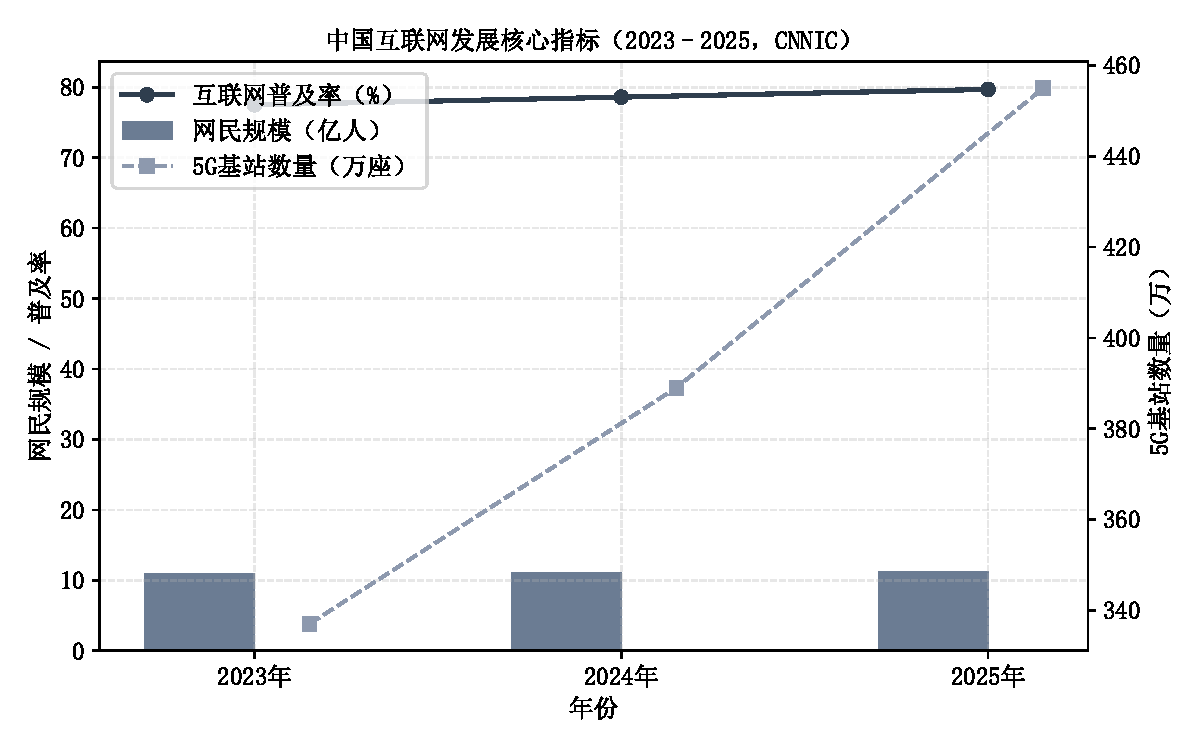
\includegraphics[scale=0.6]{fig/chapter1/cnnic_2025_trend.pdf}
	\caption{中国网民规模和互联网普及率（2023–2025年）}
	\label{fig:11}
\end{figure}

在网络快速发展的同时，网络安全威胁也呈现出数量激增和形态演化
的趋势。传统以单点漏洞利用为主的攻击方式逐渐向多阶段、跨平台
、隐蔽性强的高级持续性威胁（APT）演进，分布式拒绝服务攻击（
DDoS）、供应链攻击、恶意软件传播和针对关键基础设施的定向攻击
频繁发生。这类攻击往往通过异常的连接行为、突发流量、通信模式
变化或持续性隐蔽通信体现出来，对金融系统、能源系统、交通系统
和政务网络造成严重威胁。网络攻击不仅会导致网络服务中断和经济
损失，还可能引发社会秩序和国家安全风险，因此对网络异常行为的
及时识别与预警已成为网络安全防护体系中的核心任务。

网络流量作为用户通信行为和网络运行状态的直接反映，是发现安全威
胁和异常行为的重要数据基础。通过对流量特征、时序变化和通信模式
的分析，可以揭示网络中潜在的攻击活动、异常访问和资源滥用现象。
异常网络流量检测技术因此成为入侵检测系统、态势感知平台和网络安
全运维的重要组成部分。然而，随着网络规模的扩大和应用类型的多样
化，传统基于规则匹配和特征签名的检测方法逐渐暴露出局限性。这类
方法高度依赖人工构建的规则库和已知攻击特征，对未知攻击和变种攻
击的适应能力不足，在高维、大规模和高速流量环境中还面临着实时性
和可扩展性问题。与此同时，加密流量比例的不断上升使得基于内容特
征和载荷分析的传统检测手段进一步受限，仅依靠协议字段和浅层特征
已难以有效刻画复杂的通信行为。

在实际网络环境中，大规模流量数据往往缺乏精确标注，异常样本稀少
且分布不均，这使得依赖标签数据的监督学习方法在训练成本、模型泛
化能力和实际部署方面受到制约。相比之下，无监督学习方法能够在无
需人工标注的条件下，从大量未标注流量中自动学习正常通信行为的统
计规律和结构特征，并将偏离这些规律的流量识别为异常，在未知攻击
检测和动态网络环境中具有更强的适应能力。近年来，自编码器、聚类
方法、孤立森林以及基于深度表示学习的无监督模型在异常检测领域取
得了显著进展，为复杂网络流量建模和异常识别提供了新的技术路径。

同时，准确可靠的异常流量检测技术对于网络资源调度、负载均衡和服
务质量保障也具有重要意义。通过对异常流量的实时发现与预警，可以
有效避免网络拥塞、服务中断和性能下降，为网络运维与安全管理提供
科学依据。更进一步，随着数字经济、工业互联网和智慧城市建设的不
断推进，构建高效、自适应的异常网络流量检测体系，对于保障关键信
息基础设施安全、维护国家网络空间安全和支撑社会数字化运行具有重
要的战略价值。

在此背景下，开展基于无监督学习的异常网络流量检测研究，不仅有助
于突破传统规则驱动和监督学习方法在复杂网络环境中的局限，而且能
够有效应对标签匮乏、攻击多样化和加密流量普及等现实挑战。通过对
网络流量的时序特征、统计特性和行为模式进行深层次建模，可以在无
需依赖已知攻击样本的情况下发现潜在威胁，提高对新型攻击、变种攻
击和隐蔽通信的检测能力，从而提升网络安全防护的智能化和自动化水
平。在复杂真实网络环境中，异常网络流量检测面临着若干关键技术瓶
颈，其中尤以异常样本稀缺和未知攻击难以识别最为突出。

（1）异常样本稀少且标注困难的问题。在实际网络运行过程中，绝大多
数流量属于正常业务通信，而异常流量通常只在攻击发生或系统异常时短
暂出现，具有低发生率和强不平衡性的特点。此外，异常流量的精确标注
往往依赖于安全专家对网络日志、流量行为和攻击过程的综合分析，不仅
人工成本高，而且在加密通信和复杂业务环境下难以保证标注的一致性与
准确性。这使得大规模、高质量的标注异常流量数据难以获得，导致基于
监督学习的检测方法在训练阶段容易出现过拟合或泛化能力不足的问题，
难以适应真实网络环境中不断变化的流量分布。

（2）未知攻击与变种攻击难以有效检测的问题。现有多数异常流量检测
和入侵检测方法依赖于历史攻击样本或预定义特征规则，对已知攻击类型
具有较好的识别能力，但当攻击者采用新的攻击手段、变更攻击特征或利
用零日漏洞时，这类方法往往失效。随着APT攻击、分布式协同攻击和隐
蔽通信技术的不断发展，攻击行为呈现出低频化、持续化和高度隐蔽的特
征，仅基于已知样本或静态规则构建的模型难以准确刻画其行为模式，容
易造成漏报和误报，从而削弱网络安全防御体系的有效性。

正是在上述两方面挑战的共同作用下，基于无监督学习的异常网络流量检
测方法逐渐成为研究热点。无监督学习无需依赖人工标注的异常样本，而
是通过对大量正常网络流量的统计特征和时序行为进行建模，自动学习正
常通信模式的内在分布结构，从而将偏离该分布的流量判定为异常。这种
以“正常行为建模”为核心的检测机制，使模型在面对异常样本稀缺和未知
攻击频繁出现的情况下仍具有较强的鲁棒性和泛化能力，能够更好地适应
复杂、动态和开放的网络环境。

综上所述，基于无监督学习的异常网络流量检测研究在理论上有助于推
动机器学习与网络安全领域的交叉融合，在技术上能够提升对未知威胁
的识别能力，在工程应用和国家安全层面则为构建智能化、可靠的网络
安全防御体系提供重要支撑，因此具有显著的学术意义和现实价值。

\section{国内外研究现状}
\subsection{异常流量检测研究现状}
随着互联网规模的不断扩大和网络应用场景的日益复杂，网络异常流量检测已
成为网络安全领域的重要研究方向。网络异常流量检测的核心目标是在海量网
络流量数据中及时、准确地识别异常或恶意行为，从而保障网络系统的安全与
稳定运行。从研究范式上看，异常流量检测通常被视为一种分类或异常识别问
题，其技术手段经历了由统计分析方法、传统机器学习方法向深度学习与集成
学习方法不断演进的发展过程。

早期的网络异常流量检测方法主要基于统计学原理，通过分析网络流量的统计
特征（如包大小、延迟、协议分布等）来识别异常行为。该类方法通常依赖于
对历史正常流量的建模，并通过设定阈值判断当前流量是否异常。典型研究如
基于置信度滤波、阈值判别及流量容量建模的方法，在检测DDoS攻击和蠕虫病
毒等显著异常行为方面取得了一定成效。统计方法计算简单、实现成本低，但
对复杂攻击和新型未知威胁的检测能力有限，且对阈值设定和历史数据依赖较
强，适应性不足。

网络异常流量检测逐渐向高维特征建模、时序关联学习和无监督检测方向发展。
相较于早期依赖人工特征和规则的方法，研究者更加关注模型对复杂攻击行为
和未知威胁的适应能力。在无监督异常检测方面，自编码器仍是研究热点之一
。Park等人提出面向网络数据包的无监督异常检测模型\cite{Park2025Unsupervised}，仅利用
正常流量进行训练，通过对抗训练降低模型对异常流量的重构能力。实验结果
表明，该方法在保持较高检测精度的同时，大幅减少模型参数量，具备较好的
实时检测潜力。然而，该类方法仍容易受到噪声特征和阈值设定的影响。

为进一步挖掘网络流量中的时序与空间特征，研究者开始将卷积神经网络与循
环神经网络进行融合。Mirsky 等人提出了基于自编码器的无监督网络入侵检
测系统 Kitsune\cite{Mirsky2018Kitsune}，该方法通过多层自编码器
对网络流量的正常行为进行建模，并利用重构误差实现异常检测。实验结果表明
，该模型在无需攻击标签的情况下，能够有效检测多种网络攻击行为，在多种真
实网络环境中表现出较高的检测准确率和良好的实时性。Lansky等人\cite{lansky2021deep}
对近年来深度学习入侵检测方法进行了系统评估，指出时空特征融合模型在复杂攻
击识别方面具有明显优势，但模型结构复杂、计算成本较高。

随着注意力机制的发展，Transformer模型逐渐被引入网络异常流量检测领域。
Shi等人\cite{Shi2022TransformerBiLSTM}将Transformer与BiLSTM相结合，实现全局特征建模与时
序依赖学习的协同优化，在不平衡数据场景下表现出更强的检测能力。Tuli 等人提出了一种基于Transformer
的无监督异常检测模型 TranAD\cite{tuli2022tranad}，该方法利用自注意力机制对时间序列数据进行建模
，能够有效捕捉网络流量中的长期依赖关系和关键特征模式。实验结果表明，Transformer结构在复杂时序异常
检测任务中具有较强的特征建模能力，为网络流量异常检测提供了新的建模思路。然而，此类模型通常对计算资源
依赖较强，限制了其在实际网络环境中的部署。

部分研究开始探索将图结构建模引入无监督异常检测任务中。Ding 等人提出了基于图自编码器的异常检测模型 
DOMINANT\cite{Ding2019DOMINANT}，通过联合建模节点属性与图结构信息，实现对异常节点的无监督检
测。实验结果表明，该方法在复杂关系数据中具有较好的检测性能和泛化能力，为将网络流量建模为图结构并开
展异常检测提供了有效思路。此外，Zerveas 等人提出了一种基于 Transformer 的自监督表示学习框架，
通过对多变量时间序列进行自监督训练，有效提升了模型在不同数据分布下的泛化能力\cite{Zerveas2021TransformerSSL}。
相关研究表明，将自监督学习与 Transformer 结构相结合，有助于缓解跨数据集场景中模型性能下降的问题，
该思想同样适用于网络入侵检测等复杂时序建模任务。

已有研究表明，基于自动化机器学习（AutoML）的数据驱动方法能够有效提升入侵与异常检测的性能。Xu 等人
提出了一种面向物联网环境的 AutoML 入侵检测方法，通过自动化模型选择与参数优化构建检测模型，在保证检
测准确率的同时增强了模型的鲁棒性与泛化能力\cite{xu2023data}。
Ozçelebi等对随机森林、XGBoost和LightGBM等方法在CIC-IDS-2017上进行了比较，发现集成模型在不平衡情况下表现出色
\cite{Ozcelebi2025EnsembleComparison}。在复杂场景中，注意力增强型LSTM与梯度提升类集成策略结合也被证明具有提升稀
有攻击检测能力的潜力\cite{SmartGrid2025Attentional}。此外，近期研究表明，通过将特征选择机制与集成学习框架相结合，
能够进一步提升入侵检测模型在不同数据集下的稳定性与泛化性能。Injadat 等人提出了一种融合混合特征选择与集成学习的入侵
检测方法，通过筛选关键特征并组合多种分类器，在多个基准数据集上验证了该方法在检测准确率和鲁棒性方面
的优势\cite{Injadat2023EnsembleFS}。

总体而言，当前网络异常流量检测研究已从基于规则和统计的方法逐步发展到
以机器学习、深度学习和集成学习为核心的智能检测阶段。尽管现有方法在检
测精度和适应性方面取得了显著进展，但在对未知攻击的鲁棒检测、异常样本
稀少、特征选择自动化以及模型复杂度控制等方面仍存在不足。因此，设计兼
顾检测性能、计算效率和泛化能力的异常流量检测方法，仍是该领域亟需深入
研究的重要方向。

\subsection{基于异常流量检测的机器学习方法}

基于异常流量的机器学习方法通过对网络流量数据进行建模与分析，实现对正常行为模式与异常行为模式的区分，
是当前网络安全领域中应用最为广泛的异常检测技术之一。该类方法通常以网络流量的统计特征、行为特征或时序
特征作为输入，通过机器学习算法对流量进行训练与判别，从而实现对异常流量的自动识别。根据是否依赖人工标
注数据以及模型结构的不同，基于异常流量的机器学习方法主要可分为有监督学习方法、无监督学习方法\cite{nassif2021machine}
以及基于深度学习的方法。 

（1）基于有监督学习的异常流量检测方法
有监督学习方法依赖于大量已标注的网络流量数据，通过学习正常流量与异常流量之间的差异，构建分类模型以实现
异常检测\cite{megantara2021hybrid}。常见的有监督学习算法包括支持向量机（Support Vector Machine，SVM）、决策树、随机森林、K
近邻算法以及朴素贝叶斯等。这类方法通常具有较高的检测精度和较强的判别能力，尤其在已知攻击类型和标签较为
完备的情况下，能够取得较为理想的检测效果。然而，在实际网络环境中，异常流量样本往往数量有限且标注成本较
高，容易导致数据集类别不平衡问题，从而影响模型的泛化能力。因此，有监督学习方法在应对未知攻击或新型异常
流量时存在一定局限性。

（2）基于无监督学习的异常流量检测方法
无监督学习方法不依赖人工标注数据，而是通过挖掘网络流量数据的内在结构和分布特征，自动识别偏离正常模式的
异常行为\cite{UnsupervisedReview2023}。该类方法通常假设正常流量在特征空间中具有较高的相似性，而异常流量则表现为离群点或低概率事件。
典型的无监督学习算法包括聚类算法（如K-means、层次聚类）、密度估计方法以及基于概率模型的方法（如高斯混
合模型）。无监督学习方法在异常标签稀缺的场景下具有较强的实用价值，能够有效发现未知异常模式，但其检测性
能在一定程度上依赖于特征选择和参数设置，且对复杂、高维流量数据的建模能力有限。

（3）基于深度学习的异常流量检测方法
随着大数据与深度学习技术的快速发展，基于深度学习的异常流量检测方法逐渐成为研究热点\cite{kim2020deep}。该类方法能够通过多
层非线性结构自动学习网络流量的高层特征表示，减少对人工特征工程的依赖。常见模型包括卷积神经网络（CNN）
、循环神经网络（RNN）、长短期记忆网络（LSTM）以及自编码器（Autoencoder，AE）等。其中，CNN在捕捉流
量空间特征方面具有优势，RNN及LSTM在处理时间序列流量数据、建模长期依赖关系方面表现突出，而自编码器则常
用于基于重构误差的无监督异常检测任务。近年来，生成对抗网络（GAN）及图神经网络（GNN）也逐渐被引入异常流
量检测领域，以提升模型对复杂网络结构和动态变化行为的建模能力。

总体而言，基于异常流量的机器学习方法在网络安全防护中发挥着重要作用。传统机器学习方法在特定场景下具有较
高的稳定性和可解释性，而深度学习方法在处理大规模、高维度和复杂时序流量数据方面展现出更强的表达能力。如
何在检测精度、计算复杂度与实际部署成本之间取得平衡，并提升模型对未知异常流量的检测能力，仍是该领域亟待
研究的重要问题。

\subsection{基于异常流量检测的深度学习方法}
随着网络环境的复杂化和网络攻击手段的不断演进，传统基于规则或浅层机器学习
的异常流量检测方法在特征表达能力和泛化性能方面逐渐暴露出局限性。深度学习
方法通过构建多层神经网络结构，能够自动从大规模网络流量数据中学习高层次、
非线性的特征表示，在异常流量检测领域展现出显著优势，已成为当前研究的主流方向之一。

早期研究主要集中于将基础神经网络结构引入异常流量检测任务。例如，Devan 
及其团队使用了前馈神经网络（Feedforward Neural Network, FNN）结合
XGBoost 特征选择方法，形成了XGBoost-FNN异常流量检测模型\cite{devan2020efficient}
，在NSL-KDD等经典数据集上取得了优于传统贝叶斯分类器和支持向量机的检测性能。同时，
Ghorbani 及其团队提出了一种基于稀疏自动编码器（Sparse Auto Encoder, SAE）
用于流量特征降维与表示学习\cite{ghorbani2022deep}，
其中SAE能够在减少特征冗余的同时保留关键判别信息，不仅提升了检测精度，
还有效降低了模型训练时间。实验结果表明，SAE 的效果优于基于随机森林和主成分分析的特征降维方法，
并且能够显著减少模型训练所需时间。

随着卷积神经网络（CNN）在图像领域取得突破性进展，此外，研究者提出了基于
网络流量图像可视化的分类方法，通过将流量数据转换为二维图像并利用机器学习
模型进行分类，从而实现对恶意流量的检测与分析。Demmesse 等人采用图像化方
式将网络流量表示为灰度图或彩色图，然后基于卷积神经网络等机器学习算法对这
些图像进行分类，有效提升了对隐匿性恶意流量的识别精度，展示了图像表示技术
在网络流量分类与异常检测中的潜力\cite{Demmesse2023ImageTraffic}。大
量实验表明，不同尺寸和构建方式的流量灰度图会对检测效果产生显著
影响，合理的图像表示有助于提升模型的识别能力，尤其在僵尸网络流量和加密流
量检测任务中表现突出。

针对网络流量天然具有时序特性的特点，循环神经网络（RNN）及其改进模型被广
泛应用于异常流量检测。RNN能够捕获流量数据中的时间依赖关系，但在处理长期
依赖问题时存在一定不足。因此，长短期记忆网络（LSTM）和门控循环单元（GRU
）逐渐成为主流选择。这类模型在NSL-KDD、UNSW-NB15等数据集上的实验结果表
明，其在二分类和多分类任务中均优于传统RNN模型，能够更准确地刻画复杂攻击行
为的时序特征。

随着单一深度学习模型在特征表达方面的局限性逐渐显现，研究者开始关注多模型融
合的异常流量检测方法。Khan 提出了 HCRNNIDS 模型\cite{khan2021hcrnnids}，
将 CNN 和 RNN结合为CRNN结构，使模型能够分别学习网络流量数据的空间特
征与时序关系，在 CICIDS2018 数据集上取得了 97.75\%的二分类准确率。该模型的性
能优于仅使用LSTM或CNN的模型，远超传统机器学习算法的对比模型。Wu等人设
计了ResBlk结构\cite{wu2020pelican}，将CNN和门控循环单元融合，并使用残差连接和批标准化技术，
在NSL-KDD 的 10折交叉验证任务中取得了 99.21\%的二分类准确率。Sinha等人\cite{sinha2020efficient}将
一维CNN和BiLSTM组成堆叠模型，在多个异常流量检测数据集上进行多分类实验，
实验结果显示，该堆叠模型的整体准确率和少数类别F1值均优于对比模型。

近年来，注意力机制的引入为异常流量检测提供了新的研究思路。通过在模型中引入
通道注意力、自注意力或多头注意力机制，可以对关键流量特征进行加权，从而提升
模型对重要信息的关注能力。Lan等研究者提出了MEMBER模型\cite{lan2022member}，该模型利用通道
注意力机制的卷积多任务学习，在多个流量异常检测领域基准数据集上取得了较高的
F1 值。Fu等研究者通过BiLSTM学习流量数据时序特征，并利用通道注意力影响特征
图，大量消融实验表明了通道注意力在异常流量检测上的有效性\cite{fu2022deep}。张安琳等研究者
使用自注意力机制对 CNN 和 BiGRU 提取的特征进行加权处理\cite{张安琳2022基于}，该方法在
CICIDS2018 数据集上的总精确率与召回率均得到提升。杨月麟等研究者提出了一种卷
积神经网络与Transformer结合的异常检测模型\cite{杨月麟2021基于深度学习的网络流量异常检测}，
并使用CReST类别再平衡算法解决数据集不平衡问题。在 CICIDS2017 数据集上实现了较高的准确率，
同时在 DoS 和Probe 等少数类别上的检测率与召回率优于对比模型。

随着深度学习方法的不断演进，越来越多研究将注意力机制、混合模型结构与自动学习能
力引入异常流量检测中，从而显著提升了检测精度与特征自动提取能力
\cite{hozouri2025comprehensive}，然而，这些方法在小样本条件下的训练效率与跨场景泛化能力仍然受到挑战。
 为此，研究者提出了结合自注意力机制的少样本入侵检测框架来增强模型鲁棒
 性与跨域适应能力\cite{xu2025few}，同时也有工作采用增量特征学
 习与相似性嵌入方法提升对未知攻击的实时检测能力\cite{alitbi2025generalized}。

\section{本文主要研究内容及创新}

\subsection{主要研究内容}
本论文主要研究内容包含三个部分，如图\ref{fig:13}所示。
\begin{figure}[h]
	\centering
	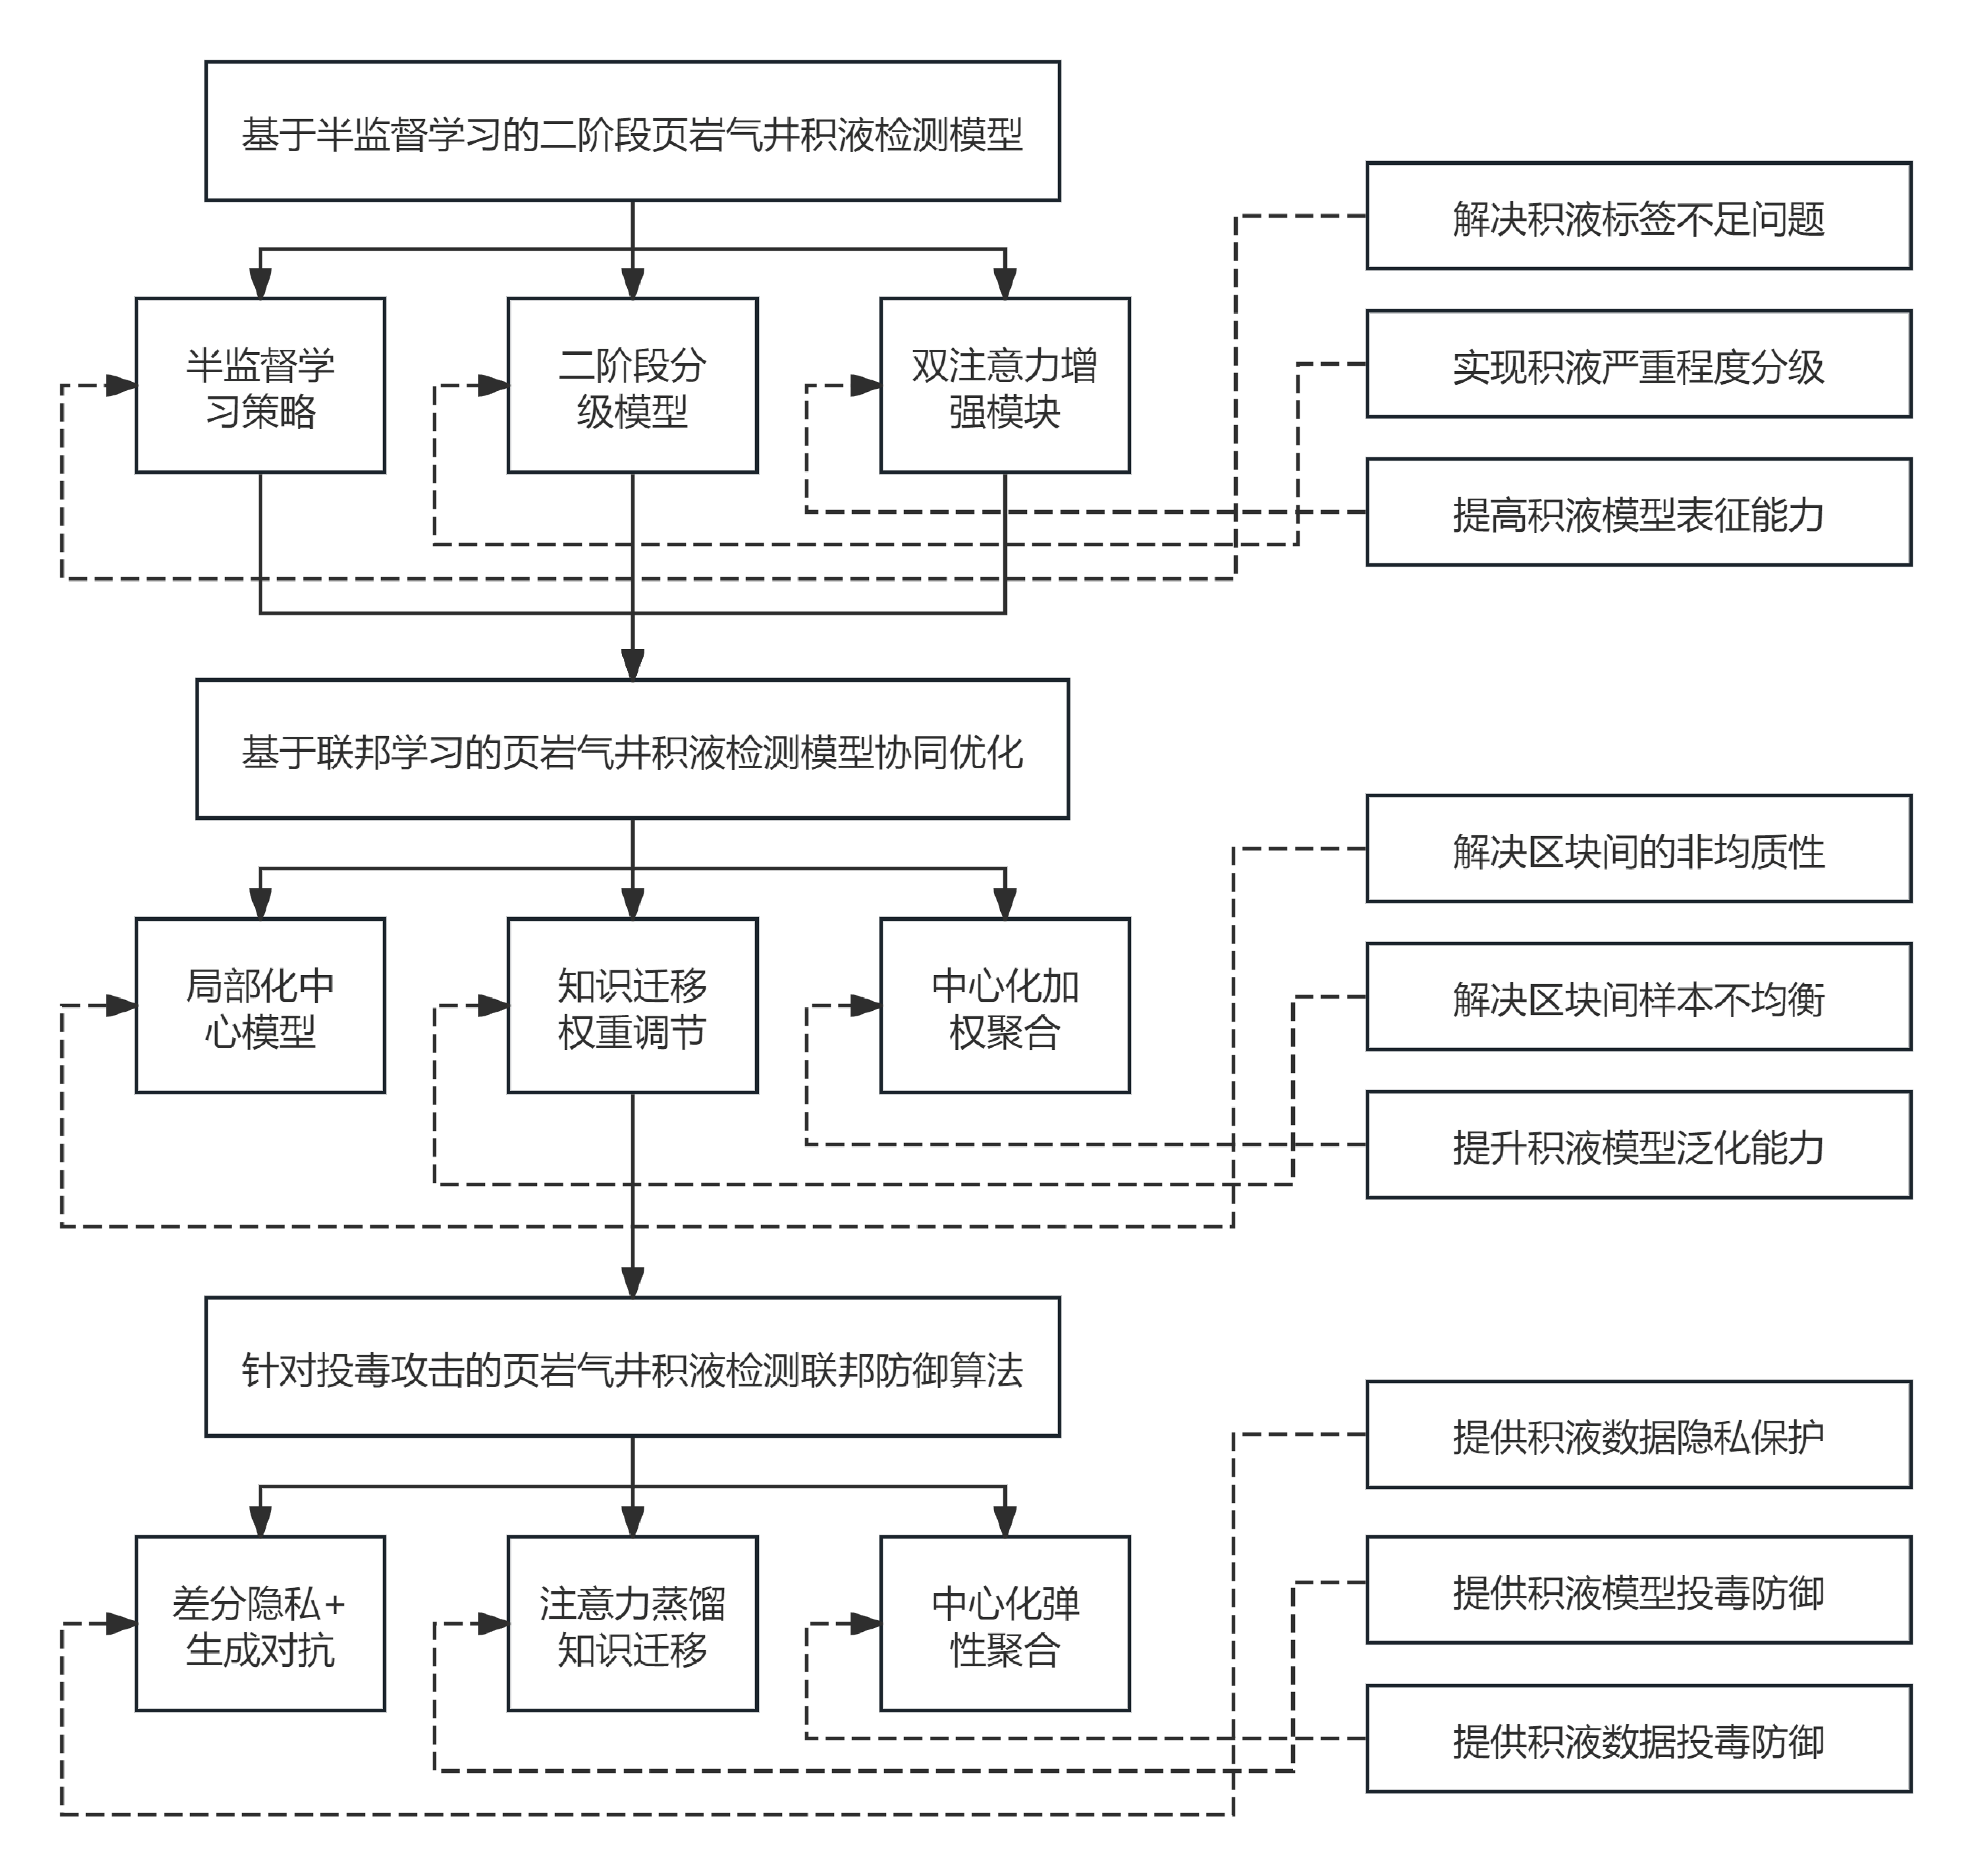
\includegraphics[width=0.8\linewidth]{fig/chapter1/图1-3.pdf}
	\caption{页岩气井积液检测场景下针对投毒攻击的联邦学习算法的研究架构}
	\label{fig:13}
\end{figure}
第一部分，我们提出了一种基于半监督学习的二阶段页岩气井积液检测模型。
该模型采用分段式设计：第一阶段通过检测积液是否存在，初步判断井筒的积液状态；
第二阶段在第一阶段的基础上，进一步对积液样本的严重程度进行分级。
这种分阶段的设计不仅提高了模型对积液状态的识别精度，还为排水措施的制定提供了量化依据。
在模型构建过程中，我们采用了半监督学习策略，充分利用少量标注数据与大量未标注数据进行训练。
该策略有效避免了大量标签制作所带来的高昂成本开销，同时借助标注数据为模型训练提供了必要的指导。
此外，我们还设计了一种双注意力增强模块，该模块强化了模型对积液特征的表征能力，
帮助模型实现更高的识别准确率。

第二部分，我们设计了一种基于联邦学习的页岩气井积液检测模型协同优化方法。
该方法为每个区块的积液检测模型设置了一个“局部化中心模型”。
该模型将从其他区块学习到的信息经过筛选，再传递到本地积液检测模型，
有效避免因区块间生产环境差异导致的模型性能下降。
此外，我们还设计了一种动态双向权重调节机制，
该机制包含中心化加权聚合算法和知识迁移权重调节算法两个部分。
中心化加权聚合算法以本地数据为参考标准，逐步整合其他区块的信息，
使积液模型在协同优化过程中保持一定个性化的同时逐步提升泛化能力。
知识迁移权重调节算法则能帮助样本量较少的新开发区块从协同优化训练中获取更多有利信息。

第三部分，我们针对投毒攻击的页岩气井积液检测联邦防御算法进行了深入研究。
在隐私保护方面，我们结合了差分隐私技术和生成对抗网络。在满足差分隐私加密强度的前提下，
降低了差分隐私技术对积液检测模型性能的负面影响。
在攻击防御方面，我们从模型投毒攻击和数据投毒攻击两个角度进行了研究。
针对数据投毒，我们在知识迁移权重调节算法的基础上，结合基于注意力蒸馏的防御算法，
形成了一种基于注意力蒸馏的知识迁移算法，
并验证了其在页岩气井积液检测模型协同优化场景下防御数据投毒攻击的有效性。
针对模型投毒，我们将拜占庭弹性聚合与中心化加权聚合相结合，
形成了一种中心化弹性聚合算法，增强了积液模型在面对恶意模型参数时的稳定性。

综上所述，本研究围绕页岩气井积液检测，
提出了一种融合半监督学习、联邦学习和隐私保护技术的综合解决方案。
通过半监督学习的二阶段检测模型，实现了积液状态的精准识别与分级。
在此基础上，借助联邦学习的协同优化，引入“局部化中心模型”和动态双向权重调节机制，
有效应对了生产环境的非均质性问题，提升了模型的泛化能力。
同时，结合差分隐私技术和生成对抗网络，优化隐私保护机制，
并通过基于注意力蒸馏的知识迁移算法和中心化弹性聚合算法，增强了模型对投毒攻击的防御能力。
该研究将积液检测的精度提升、模型优化与隐私安全防护有机结合，
为页岩气井的高效管理和安全运营提供了全面的技术支撑。

\subsection{主要创新}
本文创新点可总结为以下三点：

（1）通过半监督学习结合有监督和无监督学习的优势，解决了标签数据不足问题，
并采用二阶段设计进行积液检测和严重程度分级，辅以双注意力增强模块提高了模型的表征能力。

（2）通过为每个区块的积液检测模型设置“局部化中心模型”来避免生产环境非均质引起的模型偏向性。
并设计动态双向权重调节机制，帮助样本量较少的区块在协同优化过程中能够获得更多的关注。

（3）通过生成对抗网络+差分隐私技术在数据隐私保护强度与积液检测模型性能之间取得较好的平衡。
结合基于注意力蒸馏的知识迁移算法和中心化弹性聚合算法，
有效识别并防御积液检测模型在联邦学习训练过程中的投毒攻击。

\section{本文组织架构}
\textbf{第一章}：介绍论文的研究背景、国内外研究现状及本文的主要研究内容与创新。
阐述了当前井筒积液检测领域中主流的物理模型和数据驱动模型；
对联邦学习技术及其最新的投毒攻击与防御研究进行了综述。

\textbf{第二章}：介绍相关技术及理论。涉及传统井筒积液检测方法和基于数据驱动的检测方法；
对有监督、无监督和半监督学习策略进行了阐述；
重点介绍了联邦学习中的投毒攻击及其主流防御策略，分析了这些策略的优缺点。

\textbf{第三章}：介绍基于半监督学习的二阶段页岩气井积液检测模型。
详细说明了本研究所使用的数据集及数据预处理过程；
展示了二阶段井筒积液分级模型的具体结构，重点介绍了双注意力增强模块；
阐述了积液模型训练所采用的半监督学习流程。

\textbf{第四章}：介绍基于联邦学习的页岩气井积液检测模型协同优化方法。
详细展示了利用局部化中心模型思想完成页岩气井积液检测模型协同优化训练的整体流程，
重点介绍了动态双向权重调节机制，包括中心化加权聚合和知识迁移调节两个部分。

\textbf{第五章}：介绍针对投毒攻击的页岩气井积液检测联邦防御算法。
评估差分隐私+生成对抗网络方法的数据隐私保护强度及其对积液检测模型性能的影响；
评估基于注意力蒸馏的知识迁移算法在协同优化训练中对数据投毒攻击的防御效果；
评估中心化弹性聚合算法在协同优化训练中对模型投毒攻击的防御效果。

\textbf{第六章}：对全文进行总结与思考，并对未来研究方向进行展望。


% !TEX root = ../swputhesis.tex
\chapter{相关技术及理论介绍}

\section{异常流量数据检测相关概念}
在网络流量异常检测领域的现有研究中，长尾分布下的数据不平衡问题与复杂环境
下的未知攻击检测是当前面临的两个核心挑战。

在长尾分布下的异常检测研究方面，传统的无监督单分类方法（如支持向量数据描
述、自编码器等）普遍基于正常流量在特征空间中紧凑分布的理想假设。然而，真
实网络中的正常流量往往呈现显著的长尾分布特性，即由海量高频的单一背景流量
构成“头部”，而由少量低频但多样的关键业务流量构成“尾部”。现有模型在优化
时不可避免地被高频头部样本主导，导致特征中心向高密度区域偏移，决策边界过
度收缩。这种偏差会使得处于长尾部分的稀疏正常流量被排斥在边界之外，从而引发极高的误报率。

在面向未知攻击的异常检测研究方面，随着零日攻击和高级持续性威胁的频发，异常
标签往往难以获取。现有的无监督聚类检测方法虽然在一定程度上摆脱了对标签的依
赖，但普遍存在单一聚类中心的理论局限。真实网络中的正常业务极其异构，往往表
现为多个独立的高密度聚集区。若强行使用单一中心拟合多中心的复杂分布，不仅会
造成处于分布边缘的合法样本被误报，更会导致潜伏在多类正常模式间隙的复杂未知
攻击成功逃避检测。


\subsection{数据包与PCAP接口}
数据包是计算机网络中进行数据传输的基本单位，它将用户需要传输的数据
与必要的控制信息（如地址、协议类型、校验信息等）按照协议规范组织在
一起，使数据能够在网络中被识别、传输、转发和接收。

\begin{figure}[h]
	\centering
	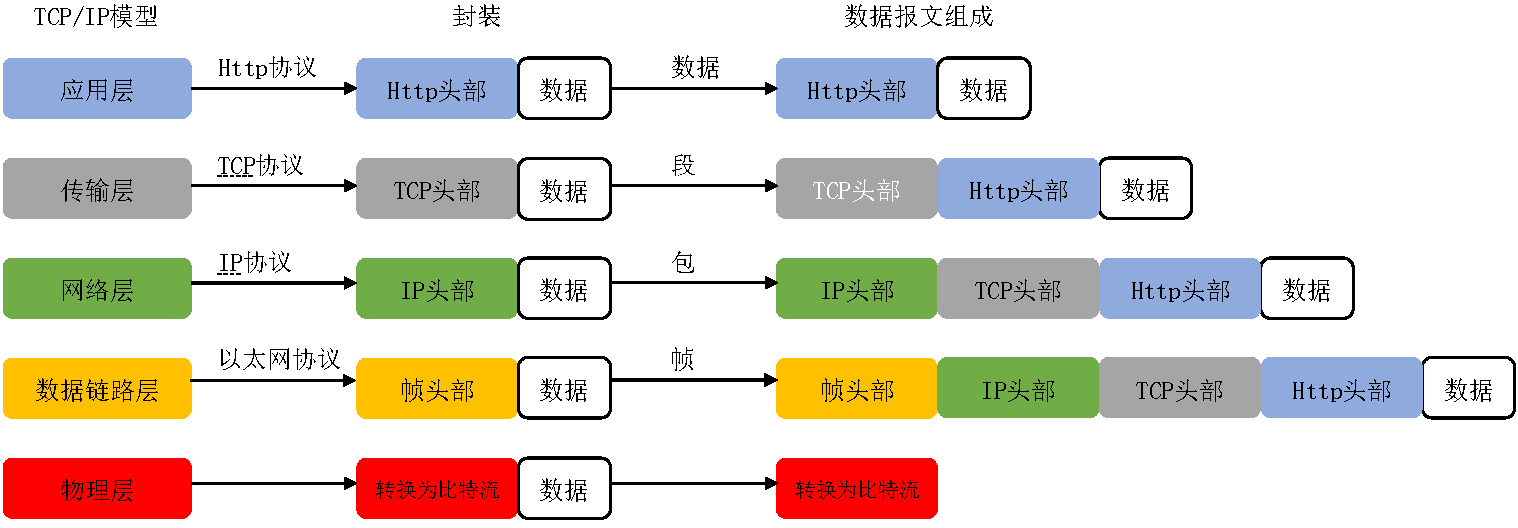
\includegraphics[scale=0.6]{fig/chapter2/数据封装过程.pdf}
	\caption{数据封装流程}
	\label{fig:2-1}
\end{figure}
在发送端，用户数据按照 TCP/IP 协议体系自上而下逐层封装：应用层对
数据进行初步封装；传输层将其封装为 TCP/UDP 数据段以实现端到端通
信；网络层加入 IP 头部形成 IP 数据包以完成路由；数据链路层将其封
装成帧；最终在物理层以比特流形式通过传输介质发送。数据封装的整体
流程如图\ref{fig:2-1}所示，主要包含五个步骤。

PCAP（Packet Capture）接口是一种用于捕获和存储网络数据包的标准化
接口与文件格式，广泛应用于网络监控、流量分析和网络安全研究等领域。它
能够在网络接口处拦截经过的数据包，并向上层应用提供统一的数据访问方式。
通过 PCAP 接口，网络监控工具（如 Wireshark、tcpdump）可以按照时间
顺序获取网络数据包，并支持使用过滤规则对流量进行筛选，从而提高捕获效率。
捕获到的数据通常以 PCAP 文件形式保存，文件由全局头和若干数据包记录组成，
每条记录包含数据包的时间戳、长度信息及原始数据内容，PCAP文件存储的信息格
式如图\ref{fig:2-2}所示。在网络异常流量检测中，PCAP 接口能够完整保留原始网络通信数
据，为后续的特征提取、行为分析和模型训练提供基础数据支持。

\begin{figure}[h]
	\centering
	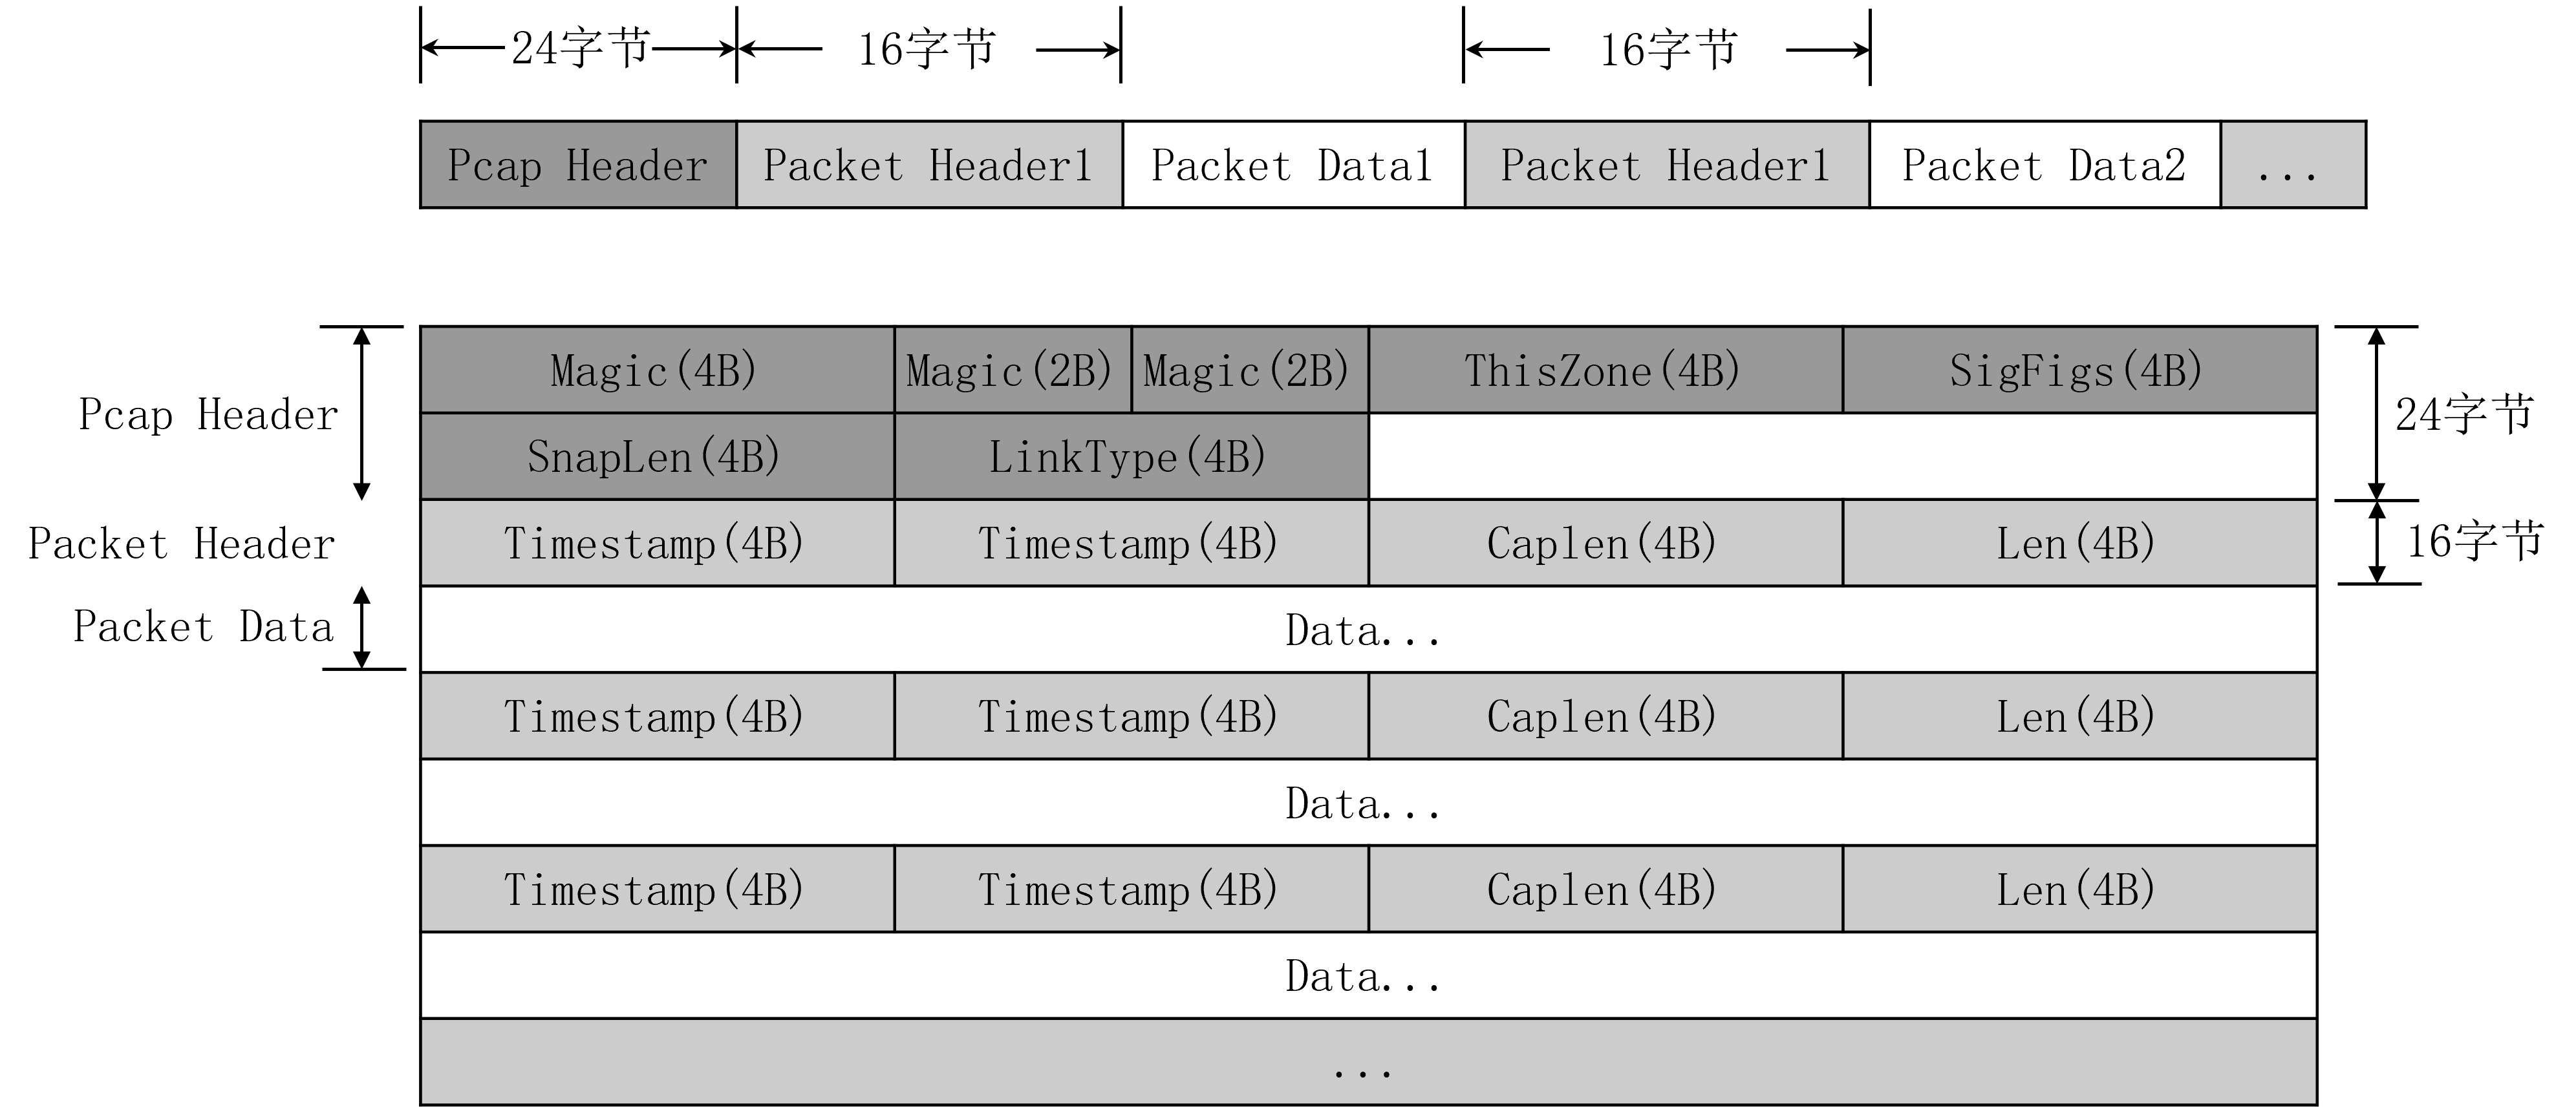
\includegraphics[scale=0.5]{fig/chapter2/PCAP文件结构.png}
	\caption{PCAP文件结构}
	\label{fig:2-2}
\end{figure}

\subsection{网络流量数据}
在网络通信中，数据包是数据传输的最小离散单位。由于单包包含的信息有限，且包与包之
间存在紧密的时序与通信关联，为更全面地刻画网络行为，研究通常以网络流作为基本分析
对象。网络流是指在特定时间窗口内，具有相同五元组（源IP、目的IP、源端口、目的端口
和传输层协议）的数据包集合\cite{1025069439.nh}。通过按五元组和时间顺序将离散数据包进行聚合，能够提取具
有明确语义的通信模式，准确反映主机间的交互特征，其聚合过程如图\ref{fig:2-3}所示。

\begin{figure}[h]
    \centering
    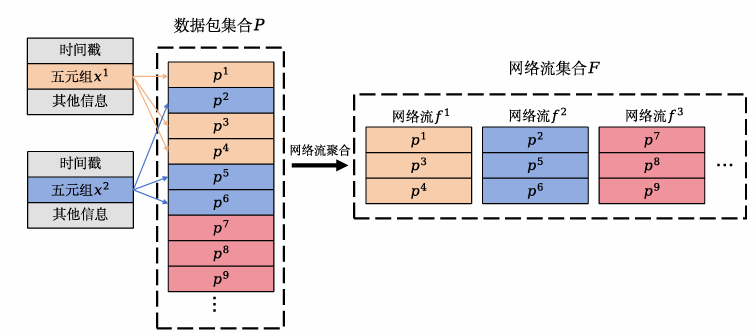
\includegraphics[scale=0.8]{fig/chapter2/网络流聚合过程.png}
    \caption{网络流聚合过程}
    \label{fig:2-3}
\end{figure}

假设某时间段内共收集了 $n$ 个数据包，可将其定义为数据包集合 $P$：

\begin{equation}
    \begin{gathered}
        P = \{p^1, p^2, \dots, p^n\} \\
        p^i = \{t^i, x^i, b^i\}, \quad i = 1, 2, \dots, n
    \end{gathered}
\end{equation}

其中，$p^i$ 表示第 $i$ 个数据包；$t^i$、$x^i$ 和 $b^i$ 分别代表该包被截获的时间戳、
五元组信息以及其他传输载荷信息。

经过网络流聚合后，离散的包集合 $P$ 被映射为包含 $m$ 条网络流的集合 $F$。每条网络
流 $f^i$ 由具有相同五元组 $x^i$ 的 $k$ 个数据包组成，并严格按时间戳递增排
序（$t^1 < t^2 < \dots < t^k$）：

\begin{equation}
\begin{gathered}
    F = \{f^1, f^2, \dots, f^m\} \\
    f^i = \{(t^1, x^i, b^1), (t^2, x^i, b^2), \dots, (t^k, x^i, b^k)\} \\
    m \le n, \quad k \le n
\end{gathered}
\end{equation}

由于总包数为 $n$，因此聚合后的网络流总数 $m$ 以及单条流内包含的数据包数量 $k$ 均不大于 $n$。

\subsection{网络攻击类型}
网络攻击是造成网络异常流量的主要原因之一。攻击行为在产生方式、通信模式以及资源消耗特征等
方面，均与正常用户访问存在显著差异，从而在网络流量中表现出明显的异常特征。根据攻击目标和
实现方式的不同，常见的网络攻击类型主要包括拒绝服务攻击、Web 攻击以及远程未授权访问攻击。

（1）拒绝服务攻击（Denial of Service，DoS）：
拒绝服务攻击通过向目标服务器持续发送大量伪造或恶意请求，占用系统计算资源、网络带宽或连接
队列，使服务器无法及时响应合法用户请求。此类攻击通常表现为流量规模突增、请求频率异常以及
连接状态异常堆积等特征，容易引发网络延迟增加、服务中断甚至系统崩溃。常见的拒绝服务攻击方
式包括 UDP 泛洪攻击、SYN 泛洪攻击以及 Land 攻击等，是异常流量检测研究中的典型攻击类型。

（2）Web 攻击：
Web 攻击主要针对 Web 应用程序及其后端服务器，利用程序设计缺陷或安全机制薄弱点实施恶意操
作。常见的 Web 攻击形式包括跨站脚本攻击（XSS）、SQL 注入和跨站请求伪造（CSRF）。此类攻
击不仅可能导致网页内容被篡改、用户会话被劫持，还可能造成数据库信息泄露或非法操作。从流量特
征角度看，Web 攻击往往表现为异常的请求参数、非正常访问路径以及请求行为模式的明显偏移。

（3）远程未授权访问攻击：
远程未授权访问攻击是指攻击者利用系统漏洞、弱口令或暴力破解等手段，在未获得合法授权的情况
下，通过远程登录方式（如 SSH、Telnet 等）侵入目标系统。一旦成功获取访问权限，攻击者可
能在受害者不知情的情况下执行数据窃取、恶意程序植入或系统控制等破坏性操作。该类攻击在网络
流量中通常表现为异常登录尝试频繁、访问时间和访问行为不符合正常用户使用习惯等特征。

\section{基于无监督学习的异常流量检测方法}
在网络安全防御体系中，由于获取带有精确标注的异常攻击样本成本高昂，且真实的流量环境
中不断涌现出未知的零日攻击，传统的有监督学习方法常常面临严重的泛化瓶颈。无监督学习
方法因其无需依赖先验标签，能够直接从海量的原始网络流量中挖掘正常行为的内在分布规律
，并将显著偏离该正常模式的流量判定为异常。这种“非正常即异常”的检测范式赋予了模型发
现未知威胁的能力。现有的无监督异常流量检测方法按照底层机制的不同，主要可划分为基于
聚类、基于边界、基于隔离以及基于深度重构四大类\cite{kozik2024survey}。

\subsection{基于聚类的检测方法}
基于聚类的检测方法是无监督异常检测中最为经典的分支\cite{kakade2024network}。
该类方法的核心假设是正常流量在特征空间中具有高度的相似性，通常会形成一个或多个高密
度的聚集类簇，而异常攻击流量则表现为游离于大类簇之外的离群点或孤立的小规模微簇。代
表性算法包括 K-Means、DBSCAN 以及高斯混合模型等，它们通过计算样本间的距离或相似
度进行无监督划分，具有较强的可解释性。然而，传统聚类算法在面对高维网络流量时容易陷
入维度灾难，且难以自适应地确定最佳的类簇数量与密度判定阈值。

为了克服单一聚类中心在复杂网络环境下的理论局限性，多中心无监督聚类建模思想被提出并广
泛应用\cite{wu2024unsupervised}。真实网络中的正常业务极其异构，该思想通过引入多
个聚类中心集合：
$$ \mathcal{E} = \{ \mathbf{e}_1, \mathbf{e}_2, \ldots, \mathbf{e}_M \} $$
以多个潜在正常行为模式共同刻画正常流量的整体分布。在这一框架下，正常样本通常至少与某一聚类
中心保持较小距离，聚集在多个相对独立或部分重叠的区域内；而异常样本则往往同时远离所有聚类中
心。这种多中心结构有效缓解了单中心模型在复杂分布下容易导致的误报与漏报问题，为更精准的异常
判别奠定了数学基础。
为更直观地说明多中心无监督聚类建模思想，图\ref{fig:无监督多中心聚类方法示意图}
给出了该方法在二维特征空间中的示意图。
如图所示，蓝色圆点表示模型学习得到的多个正常行为模式聚类中心：
\begin{figure}[h]
	\centering
	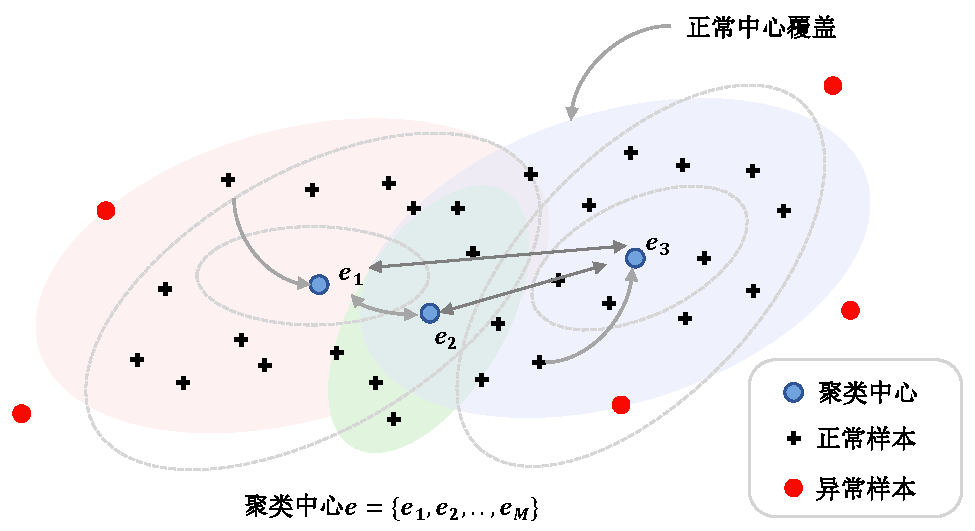
\includegraphics[scale=0.7]{fig/chapter4/多中心聚类方法示意图.pdf}
	\caption{无监督多中心聚类方法示意图}
	\label{fig:无监督多中心聚类方法示意图}
\end{figure}

\subsection{基于边界的检测方法}
基于边界的检测方法旨在特征空间中构建一个尽可能紧凑的闭合决策边界或包络面，将绝大多数的正常
流量样本包裹在边界内部，在推理阶段落在该边界之外的新样本即被判定为异常。典型的代表算法包括
单分类支持向量机与支持向量数据描述\cite{gondim2023applying}。这类方法具备坚实的统计学
习理论基础，并可通过核技巧有效处理数据的非线性映射问题。但在面对具有显著长尾分布特性或极端
不平衡的海量网络流量时，其寻优过程容易被高频的单一正常模式主导，导致决策边界过度收缩或发生
偏移，从而难以兼顾处于长尾部分的低频稀疏正常业务流。

\subsection{基于距离的检测方法}
基于距离与隔离的检测方法主要利用了异常数据在统计学和空间分布上“少且不同”的本质特征。
例如，孤立森林及其针对高维与时序流数据的隔离变体\cite{yepmo2024leveraging}，通
过随机选择特征维度与设定切分值来构建隔离树，使得分布在边缘区域的异常流量因较短的平均
路径长度而被迅速孤立。此类方法无需计算复杂的全局距离，具有极低的线性时间复杂度，非常
适合大规模流式网络数据的实时处理\cite{maspo2026anomaly}，但难以有效捕获深层的时序依赖。

在距离度量领域，为了更准确地刻画样本在特征空间中的分布状态并处理不平衡数据，实例欧氏距离（IED）
常被作为量化局部密度特征的核心工具。对于给定样本 $x_i$，其 IED 值定义为该样本与其在特征空间
中 $k$ 个最近邻样本的平均欧氏距离\cite{pang2025imbalanced}。其数学表达式如下：
$$ D_{IED}(x_i) = \frac{1}{k} \sum_{x_j \in \mathcal{N}_k(x_i)} \left\| \phi(x_i) - \phi(x_j) \right\|_2 $$
其中，$\mathcal{N}_k(x_i)$ 表示样本 $x_i$ 在特征空间中的 $k$ 近邻集合，$\phi(\cdot)$ 
为将原始数据映射到隐层空间的特征表示函数。

IED 值直接反映了样本的局部空间密度：低 IED 值对应位于密集中心的高频“头部”正常流量；高 IED 值则
对应位于稀疏边缘地带的多样化“长尾”正常模式。这一客观量化指标为在完全无监督条件下评估样本稀缺性、动
态调整模型训练权重提供了可靠的标准。

\subsection{基于深度重构的检测方法}
基于深度重构的检测方法随着现代神经网络的发展已逐渐成为当前学术界的研究主流\cite{jian2023robust}。
此类方法主要利用自编码器、变分自编码器或生成对抗网络等深度架构，在无标签的正常流量数据上进行表征压
缩与重建训练\cite{bahlali2025self,zhang2024unsupervised}。模型被迫学习正常流量的高阶非线性
特征与底层低维流形结构。在实际检测阶段，由于模型仅掌握了正常模式的重构规律，当输入未见过的异常攻击
流量时，网络往往无法完美还原输入，从而产生显著偏高的重构误差。此类方法在处理高维、高并发以及复杂
异构的网络流量方面展现出了卓越的表征学习能力。

\section{本章小结}
本章主要介绍了网络异常流量检测涉及的相关基础概念与核心检测理论。首先，深入分析了
当前异常检测领域面临的两大核心挑战：长尾分布下的数据不平衡问题与复杂环境下的未知
攻击检测问题。随后，从底层数据出发，详细阐述了数据包的封装过程、PCAP 接口的捕获
机制，以及离散数据包向网络流聚合的数学表达，为后续的特征提取与模型训练提供了数据
层面的理论基础。同时，梳理了导致网络异常的典型攻击类型，包括拒绝服务攻击、Web 
攻击和远程未授权访问攻击及其流量特征。

在此基础上，本章重点探讨了基于无监督学习的异常流量检测方法，将其系统划分为基于聚类、
基于边界、基于距离以及基于深度重构四大主流分支，并客观分析了各类方法的优势与局限性。
针对真实网络流量中呈现的复杂异构分布与长尾特性，本章进一步详细论述了多中心无监督聚
类建模思想以及基于实例欧氏距离（IED）的局部密度度量理论。这两项理论的引入，有效弥补
了传统单分类或单中心模型在处理高频背景流量与低频稀疏正常业务时的缺陷，为后续章节中解
决未知攻击检测和长尾数据不平衡问题奠定了坚实的数学与理论基础。
% !TEX root = ../swputhesis.tex
\chapter{基于多样性加权的无监督超球体网络流量异常检测方法}

\section{引言}
在网络流量异常检测任务中，无监督学习方法通常假设正常流量在特征空间中具有紧凑的分布，
而异常流量则分布在远离密集区域的稀疏空间。然而，在真实的工业互联网或企业网络环境中
，数据不平衡（Data Imbalance）问题不仅存在于正常与异常样本之间，更广泛存在
于正常流量内部\cite{lee2025madcluster}。

正常业务流量往往呈现出显著的长尾分布（Long-tailed Distribution）特征：绝
大多数流量由高频、模式单一的背景流量（如心跳包、周期性轮询）组成，这类样本构成了分
布的“头部”；而少量的关键业务操作（如大文件传输、特定数据库查询）虽然发生频率低，但
模式多样且离散，构成了分布的“尾部”。

传统的基于距离的单类分类方法（如 SVDD、自编码器）在优化过程中，往往被“头部”样本主
导，导致学习到的超球体中心过度偏向高密度区域，从而无法覆盖“尾部”的稀疏正常样本。这
导致那些稀有但正常的合法流量被错误识别为异常，引发高误报率。

针对上述问题，本章提出一种基于实例多样性加权的无监督超球体学习方法。构建了多
样性感知加权损失函数，旨在平衡不同频次正常模式对模型训练的贡献，从理论层面解决长尾
分布带来的检测偏差问题。

\subsection{无监督异常检测中的长尾分布特性}
假设训练数据集 $\mathcal{X} = \{x_1, x_2, \ldots, x_N\}$ 仅包含正常流量样本。
在理想情况下，所有样本 $x_i$ 应均匀分布在某个紧凑的流形空间上。
然而，在实际网络环境中，样本的分布密度 $\rho(x)$ 往往呈现出显著的不均衡特性。因此，
可以将正常样本集合进一步划分为两个子集：

高频正常样本集（Head Set，$\mathcal{H}$）：  
    该部分样本数量庞大，在特征空间中分布密集，
    其样本密度较高，即 $\rho(x)$ 较大，
    通常满足 $|\mathcal{H}| \gg |\mathcal{T}|$。

长尾正常样本集（Tail Set，$\mathcal{T}$）：  
    该部分样本数量较少，在特征空间中呈稀疏分布状态，
    其对应的样本密度较低，即 $\rho(x)$ 较小。

主流的自监督或无监督异常检测模型通常致力于最小化样本特征
$\phi(x)$ 到特征中心 $c$ 之间的距离，其通用目标函数可表示为：
\begin{equation}
\mathcal{L}_{\text{base}} = 
\frac{1}{N} \sum_{i=1}^{N} \left\| \phi(x_i) - c \right\|^2 .
\end{equation}

由于高频正常样本集合 $\mathcal{H}$ 的样本数量
$N_{\mathcal{H}}$ 远大于长尾样本集合 $\mathcal{T}$ 的样本数量
$N_{\mathcal{T}}$，在最小化整体损失的过程中，
模型的梯度更新方向将不可避免地受到 $\mathcal{H}$ 集合的主导。
由此带来如下三方面问题：

中心偏移（Center Bias）：  
特征中心 $c$ 会被大量高频样本强行拉向其几何中心位置，
难以兼顾分布稀疏但语义合理的正常样本。

边界收缩（Boundary Shrinking）：  
为适配高密度区域样本，模型倾向于缩小超球体半径 $R$，
从而使决策边界过度贴合主流样本分布。

尾部丢失（Tail Missing）：  
属于长尾集合 $\mathcal{T}$ 的正常样本往往位于超球体边界之外，
其异常得分（Anomaly Score）被显著放大，
从而被错误判定为异常样本，产生较高的误报率。

\begin{figure}[h]
	\centering
	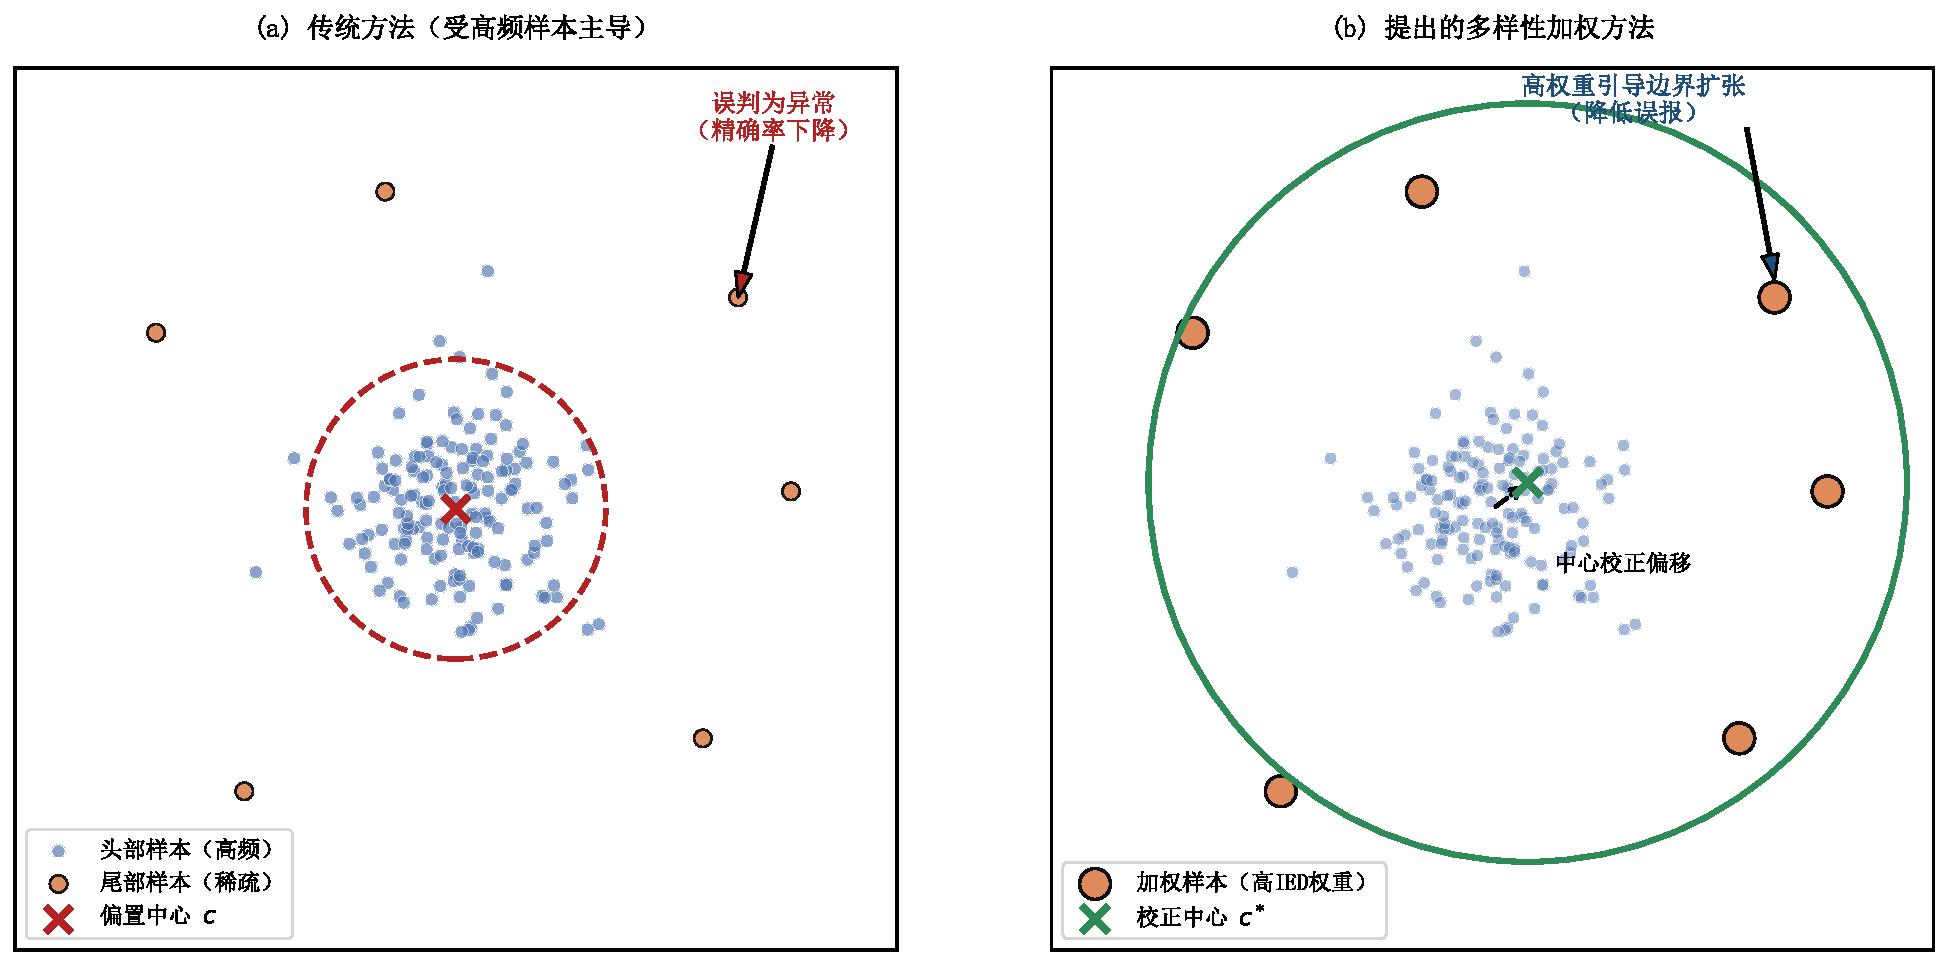
\includegraphics[scale=0.5]{fig/chapter3/传统损失函数与加权损失函数差异.pdf}
	\caption{传统损失函数与加权损失函数差异}
	\label{fig:31}
\end{figure}

如图 \ref{fig:31} 所示，传统损失函数与加权损失函数在处理不平衡数据时
呈现出明显差异：左图中，传统方法学习得到的中心点
紧贴高密度样本区域，导致灰色稀疏正常样本被误判为异常；
而右图所示的加权方法通过调节样本贡献权重，
使特征中心适度向稀疏区域偏移，从而能够覆盖多种正常模式，
有效缓解长尾样本误判问题。

为了解决上述中心偏移问题，首要任务是找到一种能够精准刻画样本处于“头部”还是“尾部”的量化指标。

\subsection{基于实例欧氏距离的样本多样性建模方法}
为有效缓解长尾分布对模型训练带来的不利影响，首先需要在无监督条件下
构建一种能够刻画样本“稀缺性”或“多样性”的度量指标。
为此，本文引入实例欧氏距离，用于量化样本在特征空间中的局部密度特征。

对于给定样本 $x_i$，其 IED 值定义为该样本与其在特征空间中
$k$ 个最近邻样本的平均欧氏距离\cite{pang2025imbalanced}。
数学表达式如下：
\begin{equation}
D_{IED}(x_i) = \frac{1}{k}
\sum_{x_j \in \mathcal{N}_k(x_i)}
\left\| \phi(x_i) - \phi(x_j) \right\|_2
\end{equation}

其中，$\mathcal{N}_k(x_i)$ 表示样本 $x_i$ 的 $k$ 近邻集合，
$\phi(\cdot)$ 为特征提取网络。

基于上述数学定义，IED的物理意义可以从样本在特征空间中的分布密度角度进行解读。
IED值的大小直接刻画了样本所处的局部密度区域，为区分不同重要性的正常流量提供了量化依据。
具体而言，IED值反映了样本在正常流量分布中的位置特征，从而揭示了不同样本对模型学习的贡献度差异。
具体表现如下：

低 IED 值：
表示 $x_i$ 位于高密度区域，周围样本相似度高，
属于“高频正常模式”（Head）。
这类样本包含的信息冗余度较高。

高 IED 值：
表示 $x_i$ 位于低密度区域，周围样本较少，
属于“长尾正常模式”（Tail）。
这类样本虽然稀少，但代表了正常业务的多样性，
对界定正常行为的边界至关重要。


通过 IED 指标，我们可以在无监督的情况下，
有效区分出哪些样本是需要模型“重点关注”的稀有正常流量。

\section{基于IED加权的超球体的异常流量检测模型}
\label{sec:weighted_method}

在明确了 IED 作为多样性度量指标的基础上，本节构建基于实例加权的自监督超球体学习模型。
该模型的核心思想是通过动态调整不同分布密度下样本的负反馈压力，引导特征空间中的超球体
边界进行自适应扩张，从而保护长尾分布下的正常样本不被误判。

\subsection{模型整体框架设计}
本章提出的方法由四个核心功能模块组成如图\ref{fig:第三章模型框架图}所示，
旨在实现从原始流量特征到具备多样性感知能力的异常度量空间的映射：

特征学习模块：针对网络流量中非平稳噪声干扰与长序列建模效率低的问题，本
模块引入小波变换与分块（Patch）机制。原始流量经离散小波变换（DWT）解耦
为全局低频与局部高频分量后，被划分为序列块并输入双分支异常注意力网络进行
特征提炼。最终输出的低维特征向量（$z$），为后续计算样本稀缺度（IED）及
优化超球体边界提供高质量的基础数据。

多样性评估模块：在每个训练批次（Mini-batch）中，利用 IED 指标实时评估样本的局
部稀缺性，识别出处于分布长尾区域的正常模式。

损失与权重模块：根据 IED 指标生成的权重因子 $w$，对损失函数进行加权更新，修正特征
中心偏移并优化超球体边界。

中心建模模块：利用上一步生成的实例权重 $w$ 计算当前批次的加权质心，并通过指数滑动平均
（EMA）策略平滑更新全局特征中心，从而主动纠正由高频样本主导的中心偏移，确保决策边界有效
包容稀疏的长尾正常模式。

\begin{figure}[h]
	\centering
	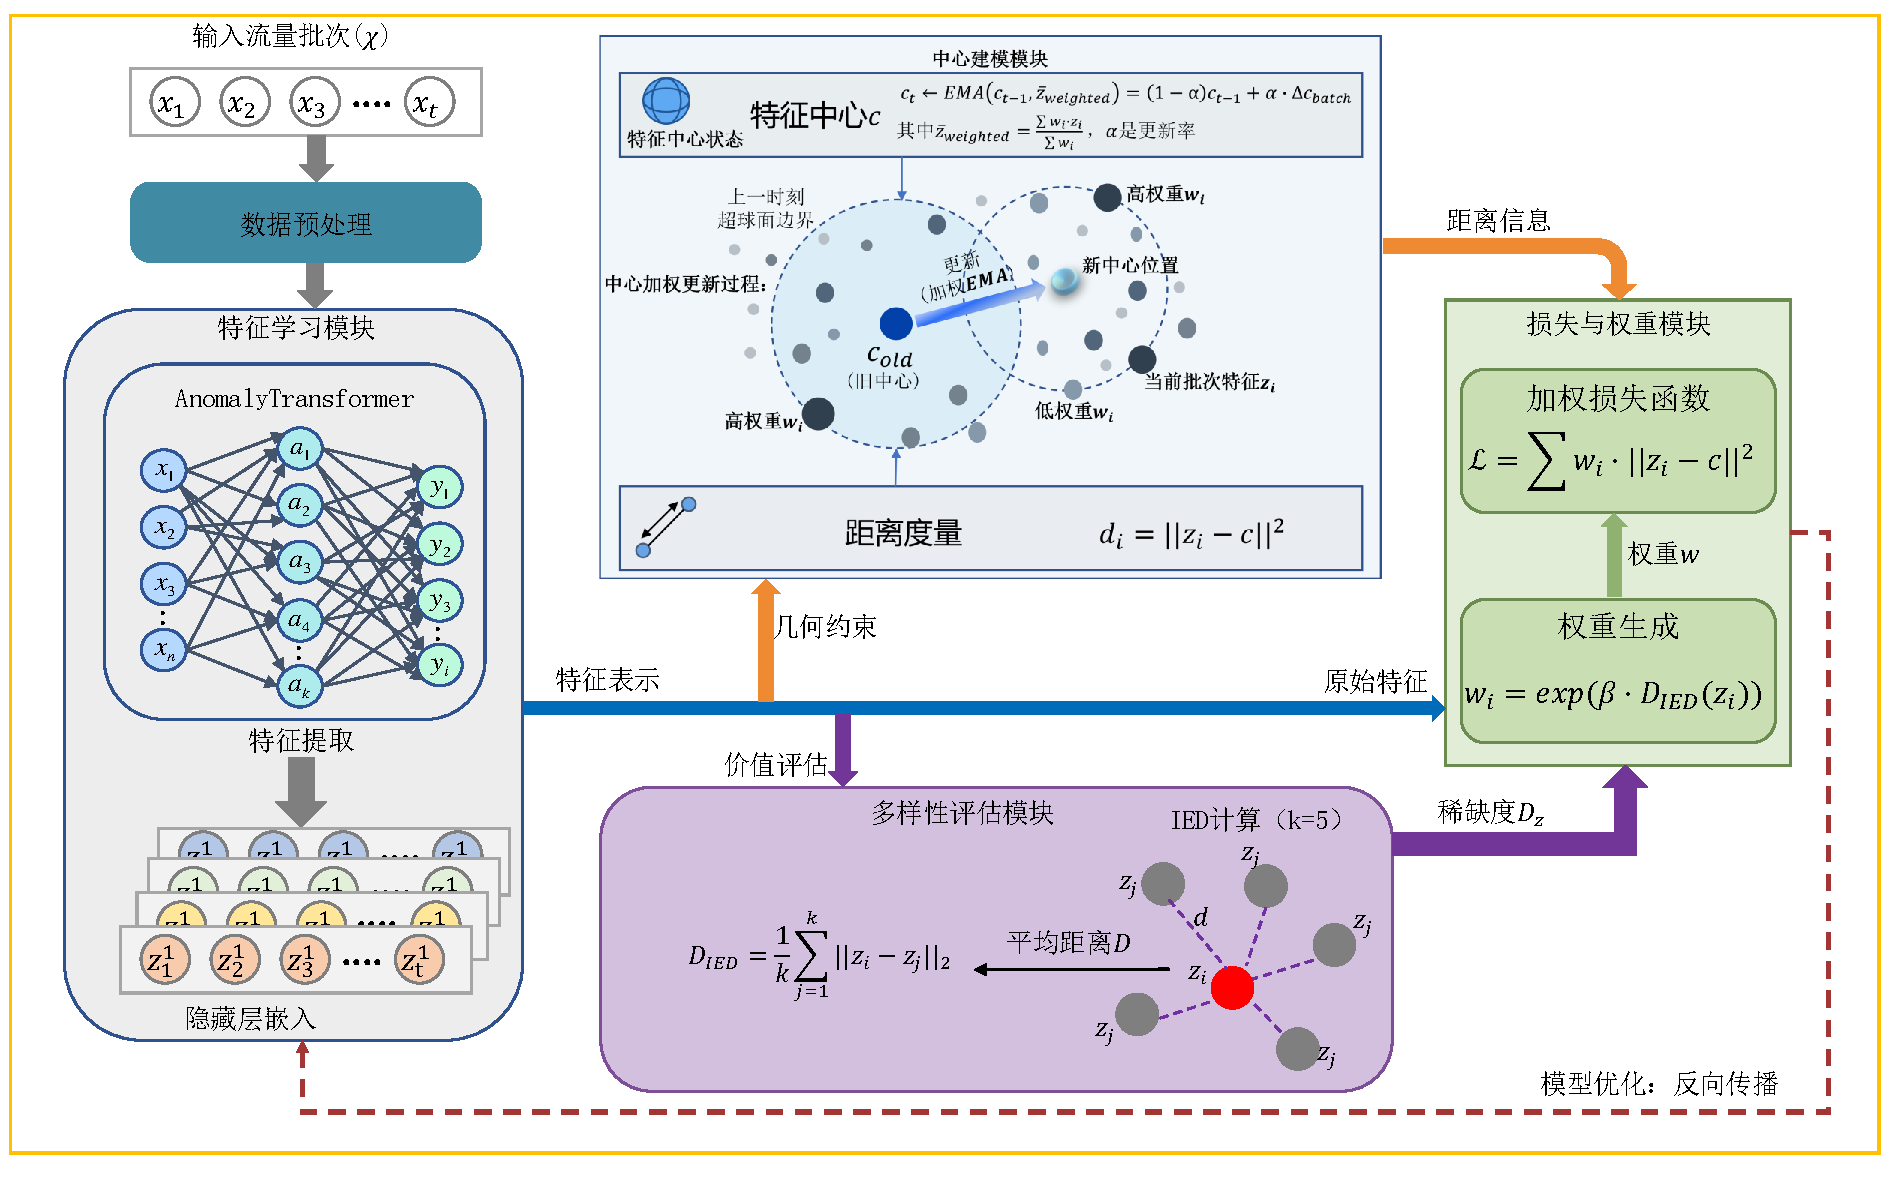
\includegraphics[scale=0.5]{fig/chapter3/第三章模型框架图.pdf}
	\caption{基于IED加权的超球体的异常流量检测模型整体框架设计}
	\label{fig:第三章模型框架图}
\end{figure}

\subsection{特征学习模块}
在网络流量异常检测任务中，原始数据常伴随复杂的非平稳噪声，且存在极长的时
序依赖。传统的逐点计算（Point-wise）Transformer 模型极易受高频噪声干
扰，且面临 $O(N^2)$ 的高昂计算复杂度。为此，本章提出一种新型的小波-分块
异常 Transformer (Wavelet-Patch Anomaly Transformer, WPAT) 模块，
创新性地将时频分析技术与序列分块机制相结合，高效提取具备极强区分度的低维流形
特征。WPAT 模块的具体处理流程如下：
\begin{figure}[h]
	\centering
	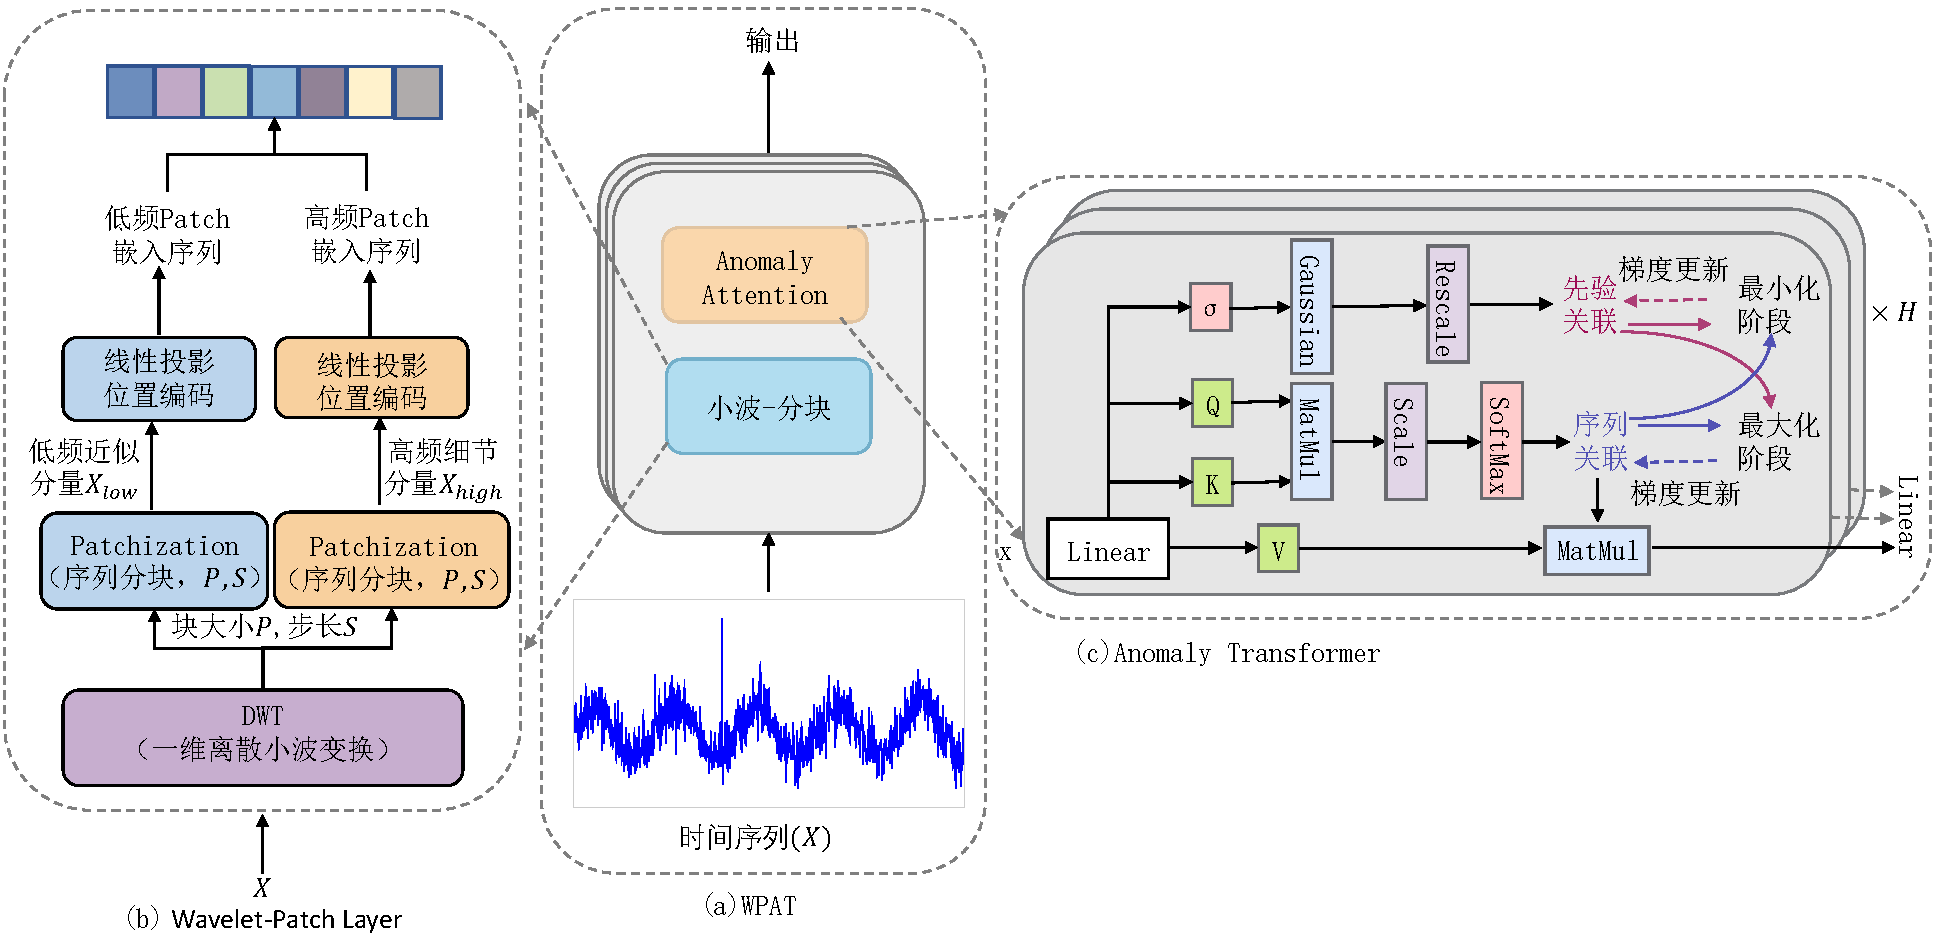
\includegraphics[scale=0.5]{fig/chapter3/WPAT特征学习模块.pdf}
	\caption{WPAT 特征学习模块}
	\label{fig:32}
\end{figure}

小波时频解耦与分块嵌入：给定预处理后的多变量流量序列 $\mathcal{X} \in \mathbb{R}^{T \times d_x}$，
首先应用一维离散小波变换（DWT）进行时频解耦，分离出表征平稳全局趋势的低频分量与捕获瞬态突变的高频分量：
\begin{equation}
    \mathcal{X}_{low}, \mathcal{X}_{high} = \text{DWT}(\mathcal{X})
\end{equation}
为提升计算效率并丰富局部语义，采用长度为 $P$、步长为 $S$ 的滑动窗口，将两分量切分为数量为 
$N = \lfloor \frac{T-P}{S} \rfloor + 1$ 的序列块（Patch）。随后通过线性投影层与位置编码，
将其映射为隐层维度为 $d_k$ 的时频 Patch 嵌入序列 $E_{low}$ 和 $E_{high}$。该机制不仅将序列
长度从 $T$ 降至 $N$，大幅降低计算开销，还赋予了特征更稳定的时间语义。

小波引导的双分支异常注意力：经典的 Anomaly Transformer 在单一时域上面临局部与全局特征提取的博弈。
本模块利用解耦后的时频 Patch 特征，显式引导双分支注意力机制的学习：

（1）低频驱动的序列关联（Series-Association）：低频分量 $E_{low}$ 滤除了噪声突变，最适合刻画全
局平稳演化规律。将其映射为查询、键、值矩阵（$Q, K, V$），通过自注意力机制计算数据驱动的序列关联权重分布：
\begin{equation}
    S_i = \text{Softmax}\left(\frac{Q_i K^T}{\sqrt{d_k}}\right), \quad i \in \{1, 2, \ldots, N\}
\end{equation}

（2）高频能量驱动的先验关联（Prior-Association）：高频分量 $E_{high}$ 直接反映流量的突变剧烈程度。
利用其动态生成先验高斯分布的尺度参数 $\sigma_i = \text{MLP}(E_{high}^{(i)})$，进而计算第 $i$ 个 
Patch 对第 $j$ 个 Patch 的先验权重：
\begin{equation}
    P_{i,j} = \frac{1}{\sqrt{2\pi}\sigma_i} \exp\left(-\frac{|j-i|^2}{2\sigma_i^2}\right)
\end{equation}
当局部出现剧烈高频波动（疑似长尾模式或异常）时，该机制能自适应地输出极小的 $\sigma_i$，迫使注意力窗口收
缩聚焦于突变上下文；而在平稳区域，则适度扩张感受野。

联合特征聚合与输出：聚合双分支的先验分布 $P_i$ 与序列分布 $S_i$，并结合特征值 $V$，再经过多层前馈网络
（FFN）与层归一化深度提炼，WPAT 最终输出低维且高度紧凑的隐层特征表示：
\begin{equation}
    \mathcal{Z} = \{z_1, z_2, \ldots, z_N\} \in \mathbb{R}^{N \times d_k}
\end{equation}
此时 $z_i$ 代表一个时间 Patch 的特征。这些具备高模式区分度的特征将作为双向输出：一方面用于多样性评估
模块计算 IED 稀缺度指标，另一方面送入中心建模模块，以优化自适应长尾正常模式的加权超球体决策边界。

\subsection{多样性评估模块}
在获取由特征学习模块输出的低维嵌入特征 $\mathcal{Z} = \{z_1, z_2, \ldots, z_t\}$ 后，
多样性评估模块的核心任务是在不依赖任何标签信息的前提下，实时量化每个样本在当前隐层特征空间中
的局部稀缺程度。该模块输出的稀缺度指标，直接决定了后续模型能否敏锐地捕捉并保护长尾分布中的稀
疏正常样本。

\begin{figure}[h]
	\centering
	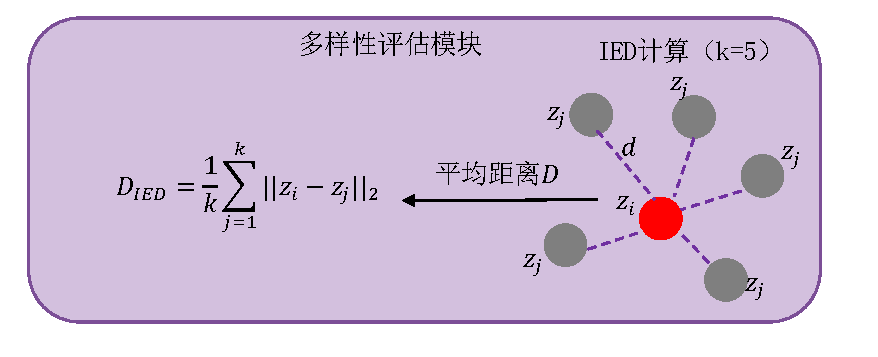
\includegraphics[scale=0.8]{fig/chapter3/多样性评估模块.pdf}
	\caption{多样性评估模块}
	\label{fig:33}
\end{figure}

如图 \ref{fig:33} 所示，该模块通过计算实例欧氏距离来完成样本价值评估。具体而言，对于当前训练批
次（Mini-batch）中的任意特征点 $z_i$，模块首先计算其与空间中其他样本点的距离，并筛选出距离
最近的 $k$ 个样本，构成局部近邻集合 $\mathcal{N}_k(z_i)$（本章模型默认设定参数为 $k=5$）。
随后，计算 $z_i$ 与该集合中所有邻居节点的平均距离，得到最终的稀缺度指标 $D_z$（即 $D_{IED}$）
。其具体的数学表达式如下：

\begin{equation}
D_{IED}(z_i) = \frac{1}{k} \sum_{j=1}^{k} ||z_i - z_j||_2, \quad z_j \in \mathcal{N}_k(z_i)
\end{equation}

参数 $k$ 的确定机制与超参数分析：

在计算实例欧氏距离的过程中，近邻数量 $k$ 是一个至关重要的超参数，其取值直接决定了多样性评估模块的灵
敏度与鲁棒性。对于 $k$ 值的确定，主要基于以下三个维度的考量：

局部感知与全局平滑的权衡：当 $k$ 值过小时（例如 $k=1$ 或 $2$），距离度量对特征
空间中的局部噪声或极端离群点极为敏感，容易将偶然的网络抖动误判为高稀缺度的长尾模式；
反之，当 $k$ 值过大时，寻找近邻的范围将不可避免地跨越不同的密度区域，导致特征的局
部密度差异被过度平滑，从而削弱了模型区分“高频头部”与“稀疏尾部”样本的边界分辨能力。

流量模式微簇的经验设定：在实际的工业网络环境中，无论是高频还是低频的正常业务流量，
在特征空间中往往以微小聚类簇（Micro-cluster）的形式存在。通过在验证集上进行的网格
搜索（Grid Search）与超参数敏感性实验，本文观察到当 $k$ 取值在 $3$ 到 $10$ 之间
时，距离指标对长尾样本的刻画最为稳定。结合具体数据集的分布特性，本章模型在整体框架中
默认设定 $k=5$。

实时检测的计算开销约束：在每个训练批次中动态计算特征距离矩阵并排序提取 $k$ 近邻，
其时间复杂度会随着 $k$ 的增大而上升。选择适中且偏小的数值（如 $k=5$），能够在确
保密度感知准确性的前提下，最大限度地控制评估模块的算力消耗，以满足网络流量异常检测
对高吞吐和低延迟的实际工程需求。

通过这种无监督的在线距离评估机制，多样性评估模块赋予了模型动态感知数据分布不平衡特性的能力。
计算得出的稀缺度 $D_z$ 将直接作为“损失与权重模块”的输入，为后续模型自适应调整优化注意力、
防止超球体决策边界过度收缩提供可靠的量化基础。

\subsection{损失与权重模块}
损失与权重模块是解决长尾样本误判问题的控制中枢，它利用多样性评估模块输出的稀缺度
 $D_z$，对模型优化过程中的惩罚力度进行自适应重分配。首先，该模块通过非线性映射函
 数将稀缺度转化为具体的实例权重 $w_i$。为了拉大“头部”与“尾部”样本对模型的不同影
 响，通常采用指数变换函数：

 \begin{equation}
 w_i=\exp(\beta\cdot D_{IED}(z_i))
 \end{equation}
 其中 $\beta$ 为温度超参数，用于控制权重的缩放尺度。权重生成后，模块将重构传统的超球体损失函数，构建
 加权损失函数：
 \begin{equation}
 \mathcal{L}=\sum w_i\cdot||z_i-c||^2
 \end{equation}

 \begin{figure}[h]
	\centering
	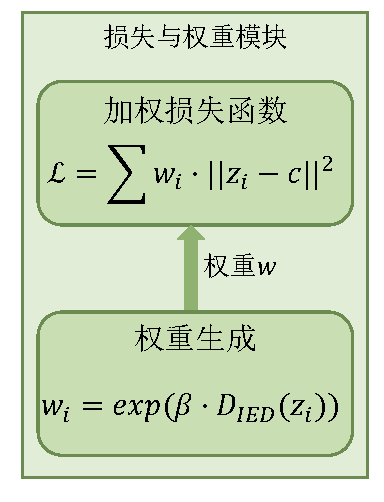
\includegraphics[scale=0.7]{fig/chapter3/损失与权重模块.pdf}
	\caption{损失与权重模块}
	\label{fig:损失与权重模块}	
\end{figure}

 在这一机制下，高频流量的
 权重被相对抑制，而长尾流量的权重被显著放大。这迫使网络在反向传播（Backpropagation）
 更新参数时，不再被数量庞大但信息冗余的头部样本主导，从而为稀疏正常样本在超球体内争取更多
 的容纳空间。

\subsection{中心建模模块}
传统的超球体模型通常采用所有样本的简单算术平均来更新特征中心 $c$，这极易导致“中心偏移”
现象。中心建模模块通过引入权重信息，实现了超球体中心的鲁棒更新，如图 \ref{fig:中心建模模块} 所示。
\begin{figure}[h]
	\centering
	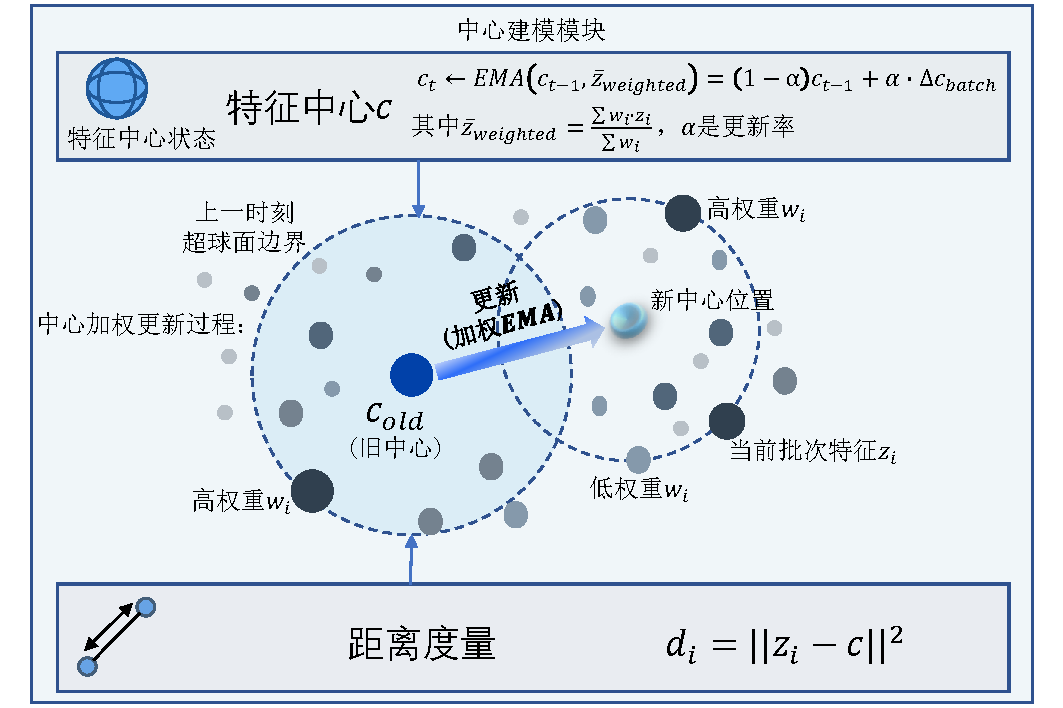
\includegraphics[scale=0.7]{fig/chapter3/中心建模框架.pdf}
	\caption{中心建模模块}
	\label{fig:中心建模模块}
\end{figure}

在每个训练批次中，该模块首先利用前序计算得到的实例权重 $w_i$，计算当前批次特征的加权质心 
$\bar{z}_{weighted}$：
\begin{equation}
 \bar{z}_{weighted}=\frac{\sum w_i z_i}{\sum w_i}
\end{equation}
随后，为了保证训练过程的稳定性并保留全局数据分布信息，模块采用指数
滑动平均（EMA）策略对全局超球体中心 $c$ 进行平滑更新：
\begin{equation}
 c_t=(1-\alpha)c_{t-1}+\alpha\cdot\bar{z}_{weighted}
\end{equation}
其中 $\alpha$ 为中心更新率。如图中直观展示的那样，高权重 $w_i$（深色节点）对“新中心位置”的拉力
更大。这一基于 EMA 和加权质心的联合更新机制，主动引导特征中心向高权重的稀疏区域适度偏移，
有效防止了决策边界的过度收缩，确保超球体能更加完整地包裹具有长尾特性的全局正常模式。

综合上述各个模块的设计，模型在每个训练迭代步骤中，通过前向传播提取时频特征并在线计算多样性权重，
随后在反向传播中利用加权损失更新网络参数，并平滑校正全局超球体中心。IED-WPAT 模型的完整训练流程
总结如算法 \ref{alg:ied_wpat} 所示。

\begin{algorithm}[htbp]
\caption{IED-WPAT模型训练算法}
\label{alg:ied_wpat}
\begin{algorithmic}[1] 
\REQUIRE 训练集 $\mathcal{X}$；批次大小 $B$；超参数 $k, \beta, \alpha, \eta$；最大轮数 $Epochs$。
\ENSURE 训练完成的网络参数 $\Theta$；全局特征中心 $c$。

\STATE 初始化参数 $\Theta$，并利用初始特征的算术平均值初始化中心 $c$；
\FOR{$epoch = 1 \to Epochs$}
    \FOR{每个批次 $\mathcal{X}_B \subset \mathcal{X}$}
        \STATE $\mathcal{X}_{low}, \mathcal{X}_{high} \leftarrow \text{DWT}(\mathcal{X}_B)$ \COMMENT{小波时频解耦}
        \STATE $\mathcal{Z}_B \leftarrow \text{WPAT}(\mathcal{X}_{low}, \mathcal{X}_{high}; \Theta)$ \COMMENT{提取隐层序列特征}
        
        \STATE $D_{IED}(z_i) \leftarrow \frac{1}{k} \sum_{z_j \in \mathcal{N}_k(z_i)} \|z_i - z_j\|_2, \forall z_i \in \mathcal{Z}_B$ \COMMENT{计算稀缺度}
        \STATE $w_i \leftarrow \exp(\beta \cdot D_{IED}(z_i)), \forall z_i \in \mathcal{Z}_B$ \COMMENT{生成实例权重}
        
        \STATE $\mathcal{L}_{batch} \leftarrow \frac{1}{B} \sum_{i=1}^B w_i \cdot \|z_i - c\|^2$ \COMMENT{计算加权超球体损失}
        \STATE $\Theta \leftarrow \Theta - \eta \cdot \nabla_{\Theta}\mathcal{L}_{batch}$ \COMMENT{反向传播更新参数}
        
        \STATE $\bar{z}_{w} \leftarrow \sum_{i=1}^B w_i z_i / \sum_{i=1}^B w_i$ \COMMENT{计算当前加权质心}
        \STATE $c \leftarrow (1-\alpha)c + \alpha \cdot \bar{z}_{w}$ \COMMENT{EMA 平滑更新全局中心}
    \ENDFOR
    
    \STATE 若验证集损失 $\mathcal{L}$ 连续无下降，则触发 Early Stopping 提前终止；
\ENDFOR

\RETURN $\Theta, c$
\end{algorithmic}
\end{algorithm}

\section{实验设置}

\subsection{实验数据集}
为了全面验证模型在多模态运维数据及复杂网络环境下的泛化能力与鲁棒性，
本文选用了五组具有代表性的基准数据集进行实验。这些数据集涵盖了服务器
性能指标（System Metrics）与网络安全流量（Network Traffic/Logs）
两大典型场景，能够充分检验 IED 加权方法在处理不同类型长尾分布时的有效性。

1. 服务器性能监控数据集

SMD (Server Machine Dataset)\cite{su2019robust}：
来源于某大型互联网公司的真实服务器集群监控系统，涵盖了为期 5 
周的连续监控记录，包含 CPU 负载、内存使用率、磁盘 I/O 等 38 
个维度的性能指标。

PSM (Pooled Server Metrics)\cite{abdulaal2021practical}：
采集自 eBay 内部的应用服务器节点，包含了 25 个维度的关键系统监控指标，
具有复杂的时序依赖性。

2. 网络安全与流量数据集

I-Sec-IDS\cite{serinelli2023toward}：该数据集模拟了复杂的内部网
络环境，包含多种混合攻击场景。其流量特征呈现典型的不平衡性，大量正常的
背景业务流量掩盖了少量的恶意横向移动或渗透行为。

AIT Alert Dataset\cite{landauer2024introducing}：来源于 
AIT Log Data Analysis 挑战赛。不同于连续的流量数据，该数据集由安全设备
的告警日志组成。在真实运营中，正常业务触发的误报（如误触规则）往往构成了高
频的“头部”，而真实的攻击行为则隐藏在稀疏的“尾部”，非常适合验证本文的长尾处理机制。

FLNET2023\cite{tayeen2023flnet}：这是一个收集于 2023 年的大规模真实网络流量数据集，
反映了现代加密流量与复杂应用层协议混合的特征。相比旧数据集，其长尾分布特征更加显著，包含大
量新型的低频应用流量。

上述数据集的统计信息如表 \ref{tab:dataset} 所示。

\begin{table}[htbp]
\centering
\caption{实验数据集统计信息}
\label{tab:dataset}
\resizebox{\textwidth}{!}{% 自适应调整表格宽度
\begin{tabular}{lcccccc}
\toprule
数据集 & 类型 & 特征类型 & 维度 ($D$) & 训练集样本数 & 测试集样本数 & 异常比例 (\%) \\
\midrule
SMD & Metrics & 纯数值 & 38 & 708,405 & 708,420 & 4.16 \\
PSM & Metrics & 纯数值 & 25 & 132,481 & 87,849 & 27.80 \\
I-Sec-IDS & Flow & 混合型 & 78 & 245,032 & 105,400 & 12.50 \\
AIT Alert & Logs & 混合型 & 19 & 45,200 & 28,800 & 2.35 \\
FLNET2023 & Flow & 混合型 & 77 & 520,100 & 310,500 & 1.25 \\
\bottomrule
\end{tabular}}
\end{table}

\subsection{数据预处理}
由于生产环境中服务器宕机、网
络波动、采集探针故障等不可抗力因素，原始数据中仍不可避免地存在
噪声干扰、数据丢失及非逻辑性数值等问题。为了消除数据质量对 IED
 加权超球体学习模型 训练的负面影响，同时保留正常流量中的长尾特征
 ，本节将按照图\ref{fig:datapreprocess}所示的流程进行严格的数据预处理。
 \begin{figure}[h]
	\centering
	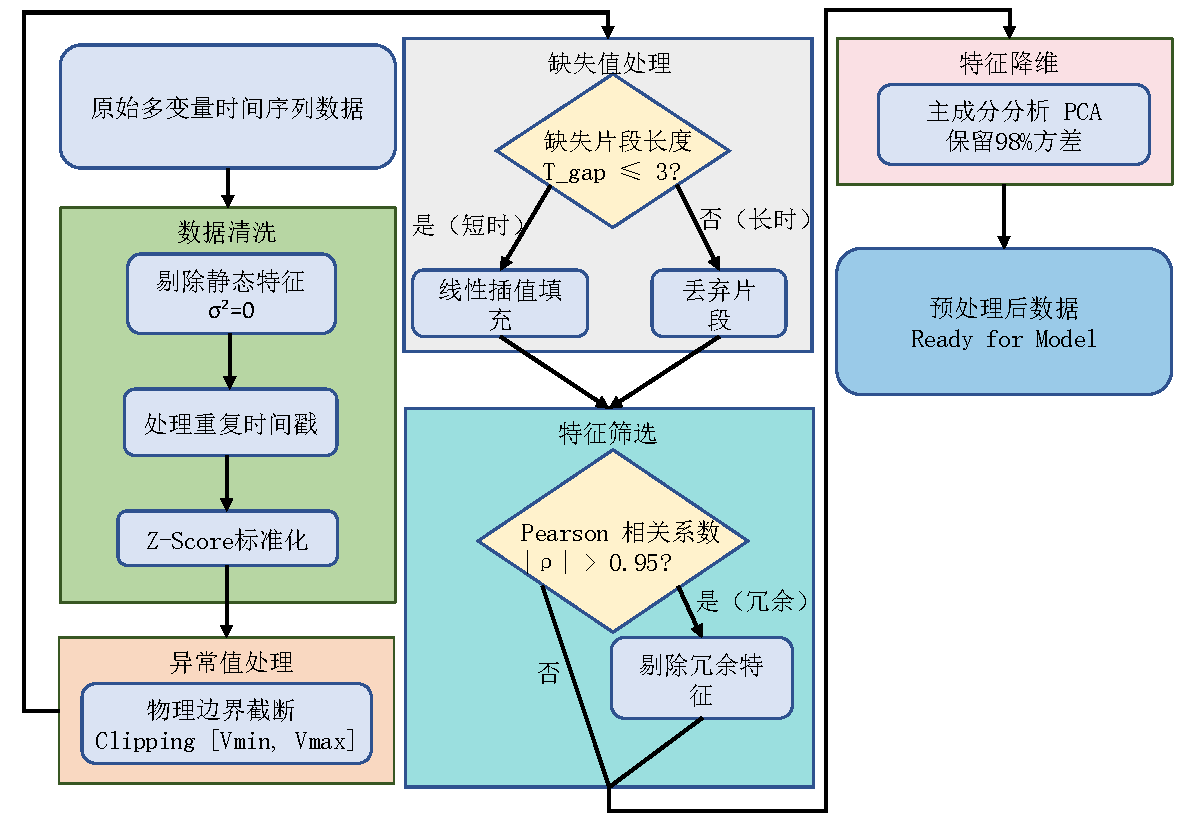
\includegraphics[scale=0.6]{fig/chapter3/数据预处理流程.pdf}
	\caption{数据预处理流程}
	\label{fig:datapreprocess}
\end{figure}

\subsubsection{数据清洗与标准化}
本阶段旨在剔除原始多变量时间序列（如 SMD/PSM 数据集）中的无效记录、
修正系统级误差并填补缺失片段，以确保输入数据的连续性与维度一致性。具
体包含以下三个处理环节：基础清洗与标准化： 首先，针对部分服务器集群
中方差为 0 的静态特征（即满足 $\sigma_j^2 = 0$ 的维度 $j$），因
其不包含有效信息且会干扰后续距离度量，将其直接剔除；其次，针对高并发
写入导致的重复时间戳，采用“保留最新”策略以维持时间序列的单调性。最后，
由于各特征（如 CPU 使用率、网络流量等）量纲差异显著，采用 Z-score 标
准化对各维特征进行归一化处理，消除大数值特征对模型度量的影响：
\begin{equation}
x'_{i,j} = \frac{x_{i,j} - \mu_j}{\sigma_j}
\end{equation}
其中，$x_{i,j}$ 
表示第 $i$ 个样本在第 $j$ 维上的原始取值，$\mu_j$ 与 $\sigma_j$ 分别为
该维度的均值与标准差。异常边界截断（Clipping）： 为严格区分“业务异常”与“系
统误差”，本阶段仅修正违反物理常识的采集错误（如 CPU 利用率超过 100\% 或网络延迟为负）
。通过为每一维特征设定物理取值边界 $[V_{\min}, V_{\max}]$，对观测值进行截断修正：

\begin{equation}
x_{i,j} = \begin{cases} V_{\max}, & 
    \text{if } x_{i,j} > V_{\max} \\ V_{\min}, & 
    \text{if } x_{i,j} < V_{\min} \\ x_{i,j}, & 
    \text{otherwise} \end{cases}
\end{equation}

此操作在修正逻辑错误的同时，完整保留了高负载等真实的“长尾”状态。缺失值分级填充： 
针对网络丢包或 Agent 重启导致的数据中断，采用分级策略以维持时序自相关性。对于短
时缺失（缺失长度 $T_{gap} \le 3$），采用线性插值保持变化趋势的连续性：
\begin{equation}
x_t = x_{t-1} + (x_{t+k} - x_{t-1}) \times \frac{1}{k+1}
\end{equation}
其中 $x_{t-1}$ 和 $x_{t+k}$ 为缺失片段前后最近的有效值；对于长时缺失
（$T_{gap} > 3$），因系统环境可能已发生突变，直接丢弃该片段及其前后相关窗口，
避免模型学习到虚假的时序依赖。

\subsubsection{特征空间优化与降维}
在完成基础数据修复后，结构化的性能指标中仍可能存在大量物理耦合的冗余信息与高
斯白噪声。为消除多重共线性并加速模型收敛，本阶段对特征空间进行进一步的筛选与降
维：基于 Pearson 相关系数的特征筛选： 为避免同一物理含义被重复计入欧氏距离度
量从而引入“维度偏见”，计算任意两维度 $i$ 与 $j$ 之间的线性相关系数 $\rho_{i,j}$：
\begin{equation}
\rho_{i,j} = \frac{\sum (x_i - \bar{x}_i)(x_j - \bar{x}_j)}
{\sqrt{\sum (x_i - \bar{x}_i)^2} \sqrt{\sum (x_j - \bar{x}_j)^2}}
\end{equation}
设定相关性阈值 $\tau = 0.95$。当 $|\rho_{i,j}| > \tau$ 时，判定两特征高度冗余，
此时仅保留方差较大的特征，剔除其余维度，从而有效压缩特征空间。基于 PCA 的主成分降维： 
为去除高斯白噪声并实现输入空间的正交化，采用主成分分析（PCA）进行特征降维。首先计算标
准化数据矩阵 $X$ 的协方差矩阵 $\Sigma$ 并进行特征值分解
（$\Sigma = \frac{1}{N-1} X^{T} X = V \Lambda V^{T}$）。
为在降维的同时最大限度保留原始结构，依据累计方差贡献率确定保留的主成分数量 
$k$：
\begin{equation}
\frac{\sum_{i=1}^{k} \lambda_i}{\sum_{j=1}^{D} \lambda_j} 
\ge \gamma
\end{equation}
实验中设置阈值 $\gamma = 0.98$（即保留 98\% 的数据方差）。
通过正交变换，不仅剔除了对应随机噪声的极小方差维度，还显著提升了特征空间的紧凑性，
为后续基于 IED 的多样性权重计算奠定了高质量的数据基础。

\subsection{评价指标}
由于网络流量异常检测本质上属于高度类别不平衡的二分类问题，
其中正常样本占据绝对多数，而异常样本极为稀缺，
因此单纯使用准确率（Accuracy）难以客观反映模型真实性能。
例如，在异常样本比例仅为 1\% 的数据集中，
若模型将所有样本均预测为正常，仍可获得 99\% 的准确率，
但该模型在实际入侵检测场景中显然是不可用的。

基于上述原因，本文选取精确率（Precision）、召回率（Recall）、
F1-Score 以及 AUC-ROC 作为核心评价指标。
所有指标均基于混淆矩阵（Confusion Matrix）进行计算，
其四种基本状态定义如下：

真正例（True Positive, TP）：  
真实的异常流量被模型正确判定为异常。

假正例（False Positive, FP）：  
正常业务流量被模型错误识别为异常，即误报。
在长尾分布场景下，大量边缘正常样本极易导致 FP 增加，
因此降低误报率是本文重点优化目标之一。

真负例（True Negative, TN）：  
正常业务流量被模型正确判定为正常。

假负例（False Negative, FN）：  
真实异常流量被模型误判为正常，即漏报，
该情况在安全场景中具有较高风险。

在此基础上，各评价指标的定义及其物理意义如下。

（1）精确率（Precision）
精确率衡量模型判定为异常的样本中，真正属于异常的比例，其计算公式为：
\begin{equation}
\text{Precision} = \frac{TP}{TP + FP}
\end{equation}

（2）召回率（Recall）
召回率表示所有真实异常样本中被模型成功检测出的比例，其定义为：
\begin{equation}
\text{Recall} = \frac{TP}{TP + FN}
\end{equation}


（3）F1-Score
F1-Score 是 Precision 与 Recall 的调和平均，用于综合评价模型在不平衡数据集上的整体性能：
\begin{equation}
F1 = 2 \times \frac{\text{Precision} \times \text{Recall}}
{\text{Precision} + \text{Recall}}
\end{equation}


（4）AUC-ROC
ROC 曲线（Receiver Operating Characteristic Curve）以假正例率
（False Positive Rate, FPR）为横轴，
真正例率（True Positive Rate, TPR）为纵轴绘制。
其曲线下的面积 AUC 定义为：
\begin{equation}
\text{AUC} = \int_{0}^{1} \text{TPR}(t)\, d(\text{FPR}(t))
\end{equation}

\subsection{参数设置}
为了确保实验结果的可靠性与可复现性，本章所有对比实验与消融实验均在统一的硬件环境与基
础参数框架下进行。模型参数分为网络结构参数、核心机制超参数以及模型训练参数三个部分，
具体设置如下：

1. 实验软硬件环境

硬件配置：所有实验均在配置有单张 NVIDIA RTX 4090 GPU（24GB 显存）和 Intel Core i9 
处理器的工作站上运行。

软件环境：操作系统为 Ubuntu 22.04 LTS，编程语言采用 Python 3.10，深度学习框架为 PyTorch 2.0，
数据处理与科学计算依赖库主要包括 NumPy、Pandas 和 Scikit-learn。

2. 核心机制超参数
本章提出的基于 IED 加权的超球体的异常流量检测模型包含三个关键超参数：

近邻数量 $k$：用于多样性评估模块计算实例欧氏距离（IED）。结合第 3.3 节的超参数分析与
验证集上的网格搜索，所有数据集均默认设定 $k=5$，以在局部感知与全局平滑之间取得最佳平衡。

温度缩放因子 $\beta$：用于控制损失与权重模块中实例权重 $w_i$ 的指数放大程度。根据数据
集长尾特性的显著程度，$\beta$ 的取值范围设定在 $[1.0, 5.0]$ 之间。对于长尾特性极强的
网络流量数据集（如 FLNET2023），$\beta$ 通常取较高值（如 3.5）；对于常规性能指标数据集
（如 SMD），$\beta$ 默认设为 2.0。

中心更新率 $\alpha$：用于控制全局特征中心 $c_t$ 的指数滑动平均（EMA）更新平滑度。为保
证训练稳定性，避免中心点随单一批次数据剧烈震荡，$\alpha$ 统一设定为 0.01。


3. 网络结构参数（WPAT）

序列分块（Patch）参数：针对不同的时间序列特性，滑动窗口长度 $P$ 依据具体数据集的周期性设定
为 16 或 32，步长 $S$ 设定为 $P/2$ 以保证相邻 Patch 之间的上下文重叠。

Transformer 结构参数：小波-分块异常 Transformer（WPAT）的隐层特征维度设定为 $d_k=512$。
双分支注意力模块采用多头注意力机制（Multi-Head Attention），注意力头数（Heads）设为8，
Transformer 编码器层数（Layers）设为 3 层，前馈神经网络（FFN）的隐藏层维度扩大至 2048。

4. 模型训练策略

优化器与学习率：模型训练采用 Adam 优化器（动量参数 $\beta_1=0.9$, $\beta_2=0.999$）。
初始学习率设为 $10^{-4}$，并引入余弦退火学习率衰减策略（Cosine Annealing）以加速后期收敛。

批次大小与迭代次数：训练批次大小（Batch Size）根据不同数据集的规模设定为 64 或 128。
最大训练轮数（Epochs）设定为 100。

早停机制（Early Stopping）：为防止模型过拟合，训练过程中引入早停机制。如果在连续 10 个 Epoch 
内，验证集上的加权损失 $\mathcal{L}$ 未出现下降，则提前终止训练，并保存具有最低验证损失的模型
权重用于最终测试。


\section{实验结果与分析}
\subsection{对比实验}

为了保证对比的广泛性，本文涵盖了从传统统计方法到最新的深度注意力机制模型：

OC-SVM (One-Class SVM)\cite{bountzis2025deep}：基于核函数的传统浅层单分类模型，作
为非深度学习方法的性能基准。

OmniAnomaly \cite{SHI2023110725}：基于随机循环神经网络（Stochastic RNN）的变分自动编
码器，利用重构概率与隐变量分布来判定异常。

USAD (Unsupervised Anomaly Detection) \cite{audibert2020usad}：结合自动编码器（AE）
与生成对抗网络（GAN）的双阶段训练框架，在工业界应用广泛。

GDN (Graph Deviation Network) \cite{deng2021graph}：利用图神经网络（GNN）显式建模传
感器之间的依赖关系，通过图注意力的偏差来检测异常。

Anomaly Transformer \cite{xu2021anomaly}：利用关联差异（Association Discrepancy）机
制捕捉长距离时序依赖，是基于 Transformer 架构的经典无监督异常检测模型。

SCAT (Spectral-Convolutional Anomaly Transformer) \cite{zhang2026scat}：
提出了一种集成频域自适应滤波与时空门控学习的统一框架。该模型通过频谱能量门控
单元（SEGU）动态抑制非平稳噪声，并利用时空门控融合（ST-Gate）协调局部与长距离时序模式，
是当前多元时间序列异常检测领域最新的 SOTA 模型。

Ours (IED-WPAT)：本文提出的基于 IED 加权的超球体异常流量检测学习方法。


\begin{table}[htbp]
\centering
\caption{不同方法在五个基准数据集上的性能对比（F1-Score / AUC-ROC，单位：\%）}
\label{tab:3-2}
\resizebox{\textwidth}{!}{
\begin{tabular}{l|cc|cc|cc|cc|cc}
\toprule
\multirow{2}{*}{模型} & \multicolumn{2}{c|}{SMD} & \multicolumn{2}{c|}{PSM} & \multicolumn{2}{c|}{I-Sec-IDS} & \multicolumn{2}{c|}{AIT Alert} & \multicolumn{2}{c}{FLNET2023} \\
 & F1 & AUC & F1 & AUC & F1 & AUC & F1 & AUC & F1 & AUC \\
\midrule
OC-SVM & 78.27 & 79.50 & 76.71 & 78.40 & 72.15 & 74.30 & 65.40 & 68.20 & 68.90 & 71.50 \\
OmniAnomaly & 88.63 & 90.12 & 89.15 & 91.05 & 84.30 & 86.50 & 76.85 & 79.10 & 81.20 & 83.45 \\
USAD & 91.79 & 93.45 & 91.63 & 92.88 & 87.65 & 89.20 & 79.50 & 82.40 & 85.10 & 87.30 \\
GDN & 93.08 & 94.80 & 93.68 & 95.20 & 89.40 & 91.15 & 82.10 & 84.60 & 87.55 & 89.80 \\
Anomaly Transformer & 94.43 & 96.10 & 95.34 & 96.55 & 91.20 & 93.40 & 85.30 & 87.90 & 89.60 & 91.25 \\
SCAT & \textbf{94.75} & 95.90 & 95.50 & 96.65 & 91.60 & 93.85 & 86.80 & 89.50 & 89.90 & 91.85 \\
\textbf{IED-WPAT (Ours)} & 94.15 & \textbf{96.25} & \textbf{95.80} & \textbf{96.90} & \textbf{92.05} & \textbf{94.10} & \textbf{88.45} & \textbf{91.20} & \textbf{90.15} & \textbf{92.40} \\
\bottomrule
\end{tabular}}
\end{table}

基于表 \ref{tab:3-2} 的实验数据，本文从长尾误报抑制、跨域泛化能力以及综合鲁棒性三个维度，
对 IED-WPAT 模型的性能优势进行深入剖析：

1. 长尾误报抑制能力

在传统的服务器性能监控场景中，本文方法在综合指标上展现了显著优势。特别是 \textbf{PSM} 
数据集，IED-WPAT 取得了 \textbf{95.80\%} 的 F1-Score 和 \textbf{96.90\%} 的 AUC，
均优于经典模型 Anomaly Transformer 及最新 SOTA 模型 SCAT。值得注意的是，在 \textbf{SMD} 
数据集中，虽然 SCAT 凭借其频谱门控机制在滤除高频噪声方面表现出色，获得了最高的 F1-Score
（94.75\%），但本文方法的 AUC 达到了最高的 \textbf{96.25\%}。AUC 指标的高低直接反映了
模型在不同阈值下对“正负样本”的排序能力。SMD 包含大量如“低频定时备份”等长尾正常行为，传统时序
模型容易将其误判为异常（导致高误报率，从而拉低 AUC）。本文方法在 AUC 上的领先，证明了 IED 加权
机制能有效缓解对稀疏正常样本的“过度敏感”，在不破坏检测边界的前提下，成功覆盖了更多的长尾正常区域。

2. 跨域泛化能力验证（网络安全数据集分析）

引入 I-Sec-IDS、AIT Alert 和 FLNET2023 数据集的目的是验证模型在网络入侵检测（NIDS）与日
志分析领域的适用性。实验结果显示，IED-WPAT 在这三个差异巨大的数据集上均取得了最优的 
F1-Score 和 AUC，证明了其强大的跨域泛化能力：

AIT Alert 数据集中，数据主要由安全设备的告警日志组成，且存在极端的长尾分布（大量重复 Head 告警 
vs 稀有 Tail 攻击）。传统模型如 OmniAnomaly 和 USAD 在此表现不佳（F1 低于 80\%），即便是经
典的 Anomaly Transformer 其 F1-Score 也仅为 85.30\%，最新的 SCAT 提升至 86.80\%。相比之
下，本文方法将 F1-Score 大幅提升至 \textbf{88.45\%}，AUC 突破 \textbf{91.20\%}。这表明通
过提升稀疏样本的权重，模型成功识别了隐藏在海量日志中的非攻击性长尾模式，显著提升了检测的准确性。

在 FLNET2023 这种大规模现代流量数据集中，网络协议的多样性极高。本文方法取得了 \textbf{90.15\%}
 的 F1-Score，优于 GDN (87.55\%)、Anomaly Transformer (89.60\%) 以及 SCAT (89.90\%)。
 这说明 IED 加权机制有效地在特征空间中为“冷门协议”保留了足够的几何空间，避免了因“高频流量主导”导
 致稀有正常流量被挤出决策边界（Decision Boundary），在复杂流量环境下仍能维持高水平的检测性能。

3. 综合性能与鲁棒性

从整体趋势来看，与当前最先进的时序异常检测模型（如 Anomaly Transformer 和 SCAT）相比，IED-WPAT
展现出了更优的综合鲁棒性。虽然 Anomaly Transformer 凭借长距离关联建模能力，以及 SCAT 凭借时空门
控与频谱自适应滤波在纯数值型数据集（如 SMD）上表现强劲，但在 \textbf{I-Sec-IDS} 等高噪声、类别极
度不平衡的混合流量数据集中，其性能增幅遭遇瓶颈（SCAT 的 F1 为 91.60\%）。相比之下，IED-WPAT 在
 I-Sec-IDS 上取得了 \textbf{92.05\%} 的 F1-Score 和 \textbf{94.10\%} 的 AUC。这得益于本
 文的超球体聚类与中心动态校正机制，该机制不仅有效滤除了背景流量中的随机噪声干扰，更从几何度量层面重
 塑了正常行为的判定基准。实验数据表明（本文方法在 5 个数据集中的 AUC 均为最高），基于IED-WPAT模型
 在处理高噪、非平稳及长尾分布数据时，具备比纯粹依赖频域滤波或时空注意力模型更强的鲁棒性与落地稳定性。


\subsection{消融实验}

为了深入探究本章提出的 IED-WPAT 模型中各个核心创新模块对最终检测性能的贡献，以及各模块之间
的协同效应，本节选取了长尾特性显著且覆盖不同应用场景的四个数据集进行消融实验。通过控制变量法，
我们设计了以下四种模型变体：

w/o WPAT：移除小波分块模块。采用标准 Vanilla Transformer 替代 WPAT，不再进行时频解耦
（DWT）与序列分块（Patch），用于验证时频解耦对非平稳噪声的抑制作用。

w/o IED：移除多样性评估与加权机制。将所有样本的损失权重强行设为 $w_i = 1$，退化为传统的无
权重超球体损失，用于验证 IED 指标对长尾分布的缓解效果。

w/o EMA：移除指数滑动平均中心更新。保留实例权重计算损失，但在更新全局特征中心 $c$ 时，采用当
前批次样本的算术平均值进行硬更新，用于验证 EMA 策略对决策边界的稳定作用。

w/o IED \& EMA（交叉消融）：同时移除实例权重与 EMA 中心更新策略。此时模型不仅不区分样本稀
缺度，中心点也仅做算术平均更新，完全退化为基于 WPAT 提取器的基础 Deep SVDD 范式，用于验证
权重分配与平滑更新机制的强耦合关系。


消融实验的定量结果如表 \ref{tab:ablation} 所示。

\begin{table}[htbp]
\centering
\caption{IED-WPAT 模型各核心模块消融实验结果对比（F1-Score / AUC-ROC，单位：\%）}
\label{tab:ablation}
\resizebox{\textwidth}{!}{
\begin{tabular}{l|cc|cc|cc|cc}
\toprule
\multirow{2}{*}{模型变体} & \multicolumn{2}{c|}{SMD} & \multicolumn{2}{c|}{PSM} & \multicolumn{2}{c|}{I-Sec-IDS} & \multicolumn{2}{c}{FLNET2023} \\
 & F1 & AUC & F1 & AUC & F1 & AUC & F1 & AUC \\
\midrule
w/o WPAT & 91.85 & 93.60 & 93.50 & 94.80 & 88.50 & 90.75 & 86.40 & 88.60 \\
w/o IED & 89.40 & 91.20 & 90.60 & 92.10 & 87.20 & 88.50 & 84.10 & 86.20 \\
w/o EMA & 93.10 & 94.85 & 94.20 & 95.30 & 90.45 & 92.60 & 88.80 & 90.50 \\
w/o IED \& EMA & 88.50 & 90.15 & 89.15 & 90.80 & 85.60 & 87.10 & 82.50 & 84.60 \\
\midrule
\textbf{IED-WPAT (Full)} & \textbf{94.15} & \textbf{96.25} & \textbf{95.80} & \textbf{96.90} & \textbf{92.05} & \textbf{94.10} & \textbf{90.15} & \textbf{92.40} \\
\bottomrule
\end{tabular}}
\end{table}

基于表 \ref{tab:ablation} 的实验数据，对各模块的作用及交叉效应剖析如下：

1. 实例多样性加权机制（IED）的决定性作用

观察实验结果可以发现，无论是在性能监控还是网络流量数据集中，当移除 IED 加权机制（w/o IED）时，
模型性能均出现了大幅下滑。尤其在长尾特征极强的 FLNET2023 数据集上，F1-Score 和 AUC 分别下降
了 6.05\% 和 6.20\%。这充分证明，在面临极端不平衡分布时，传统超球体模型由于被高密度“头部”正常
流量主导，导致决策边界发生了严重的“过度收缩”。IED 模块通过动态量化样本稀缺度并赋予高负反馈惩罚，
强制特征空间为尾部正常模式保留了足够的几何容纳量，是本文抑制高误报率的最核心机制。

2. 交叉协同效应：权重分配与中心平滑的强耦合（w/o IED \& EMA）

本实验特别设计的交叉消融变体（w/o IED \& EMA）在所有数据集上表现垫底，其性能衰减幅度远超单一模
块缺失的叠加。以 I-Sec-IDS 为例，该变体的 F1-Score 直接跌至 85.60\%。当模型同时丧失了针对稀
疏样本的权重倾斜以及对特征中心的平滑控制时，模型退化为盲目拟合高频数据的状态。反观 w/o EMA 变体
，虽然保留了权重，但由于缺乏 EMA 的“抛锚”稳定作用，少数极端稀缺样本会导致批次内的加权中心发生剧烈
跳变（即过拟合尾部噪声），使得整体性能依然存在 1\%~2\% 的损耗。这证明 IED 加权与 EMA 中心更新
在逻辑上是高度自洽、缺一不可的：IED 负责“拓宽边界”，而 EMA 负责“稳定底盘”。

3. 小波分块注意力模块（WPAT）的抗噪提炼能力

在替换为传统 Transformer 后（w/o WPAT），模型在复杂网络流数据集（I-Sec-IDS、FLNET2023）上
的性能下降尤为显著。由于混合流量中充斥着非平稳的高频抖动，逐点自注意力机制极易将其误认为异常语义。
WPAT 通过离散小波变换（DWT）将平稳趋势（低频）与突变事件（高频）显式解绑，并利用 Patch 机制扩
大了感受野。这种高质量、高紧凑度的低维特征表示，为后续欧氏距离的精确度量和超球体优化排除了“维度灾
难”与高斯白噪声的干扰。

\begin{figure}[h]
	\centering
	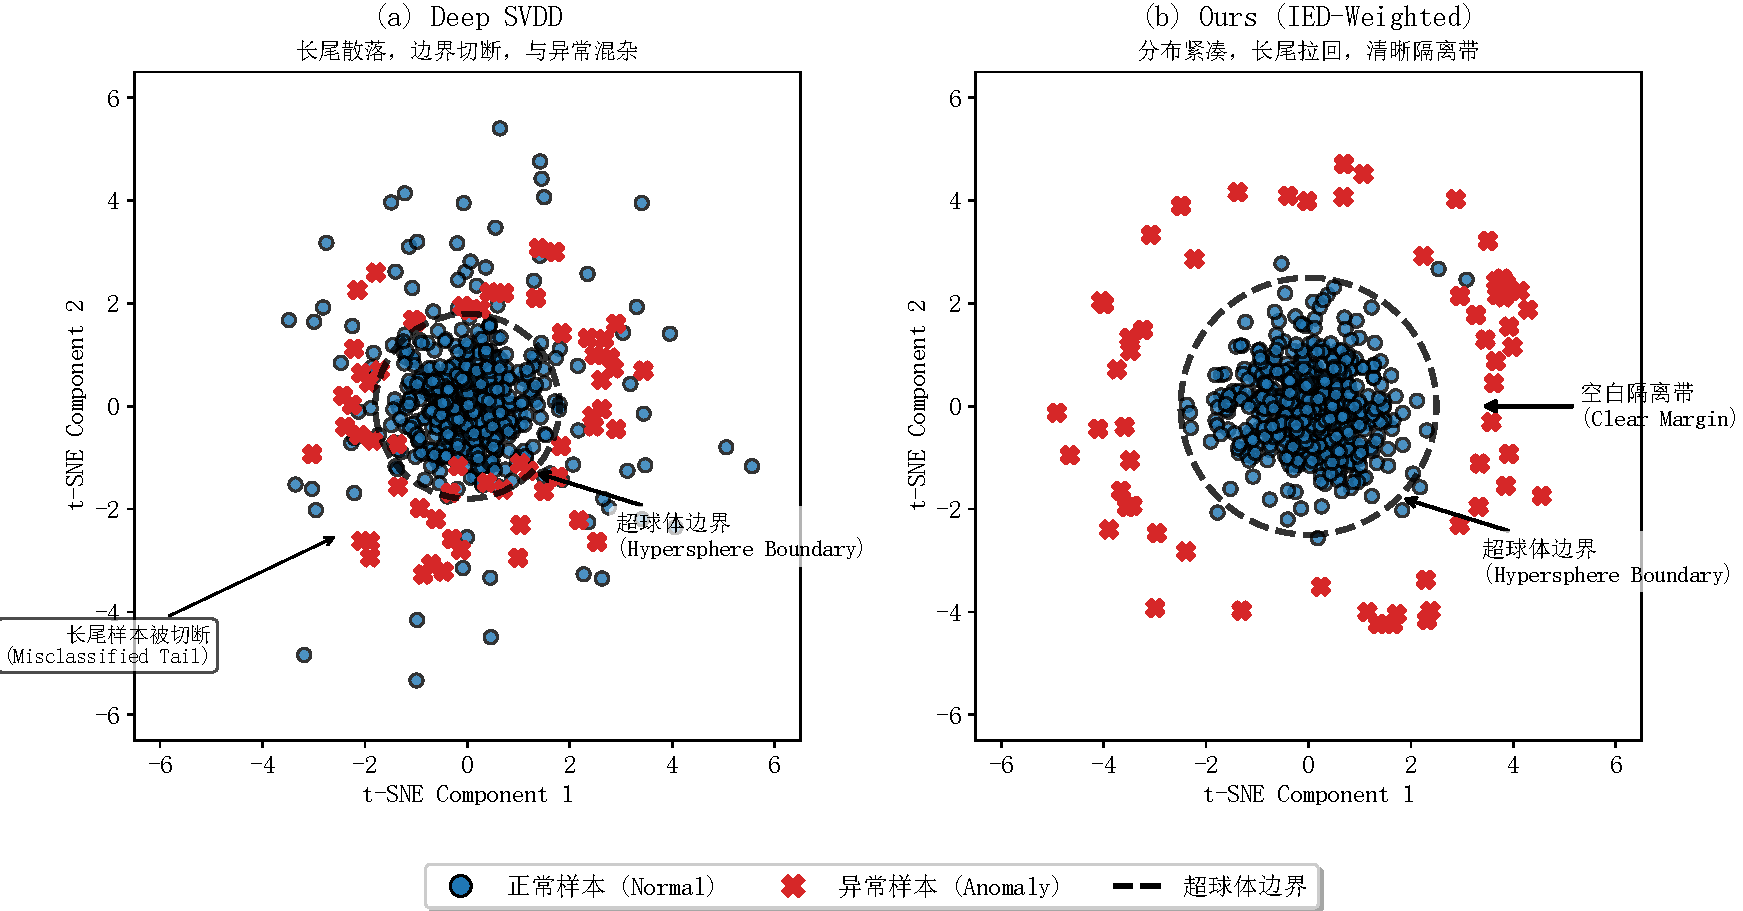
\includegraphics[scale=0.5]{fig/chapter3/t-SNE.pdf}
	\caption{数据集特征空间t-SNE可视化对比}
	\label{fig:t-SNE}
\end{figure}

特征空间分布的几何解释，为进一步验证上述量化分析，本文对不同模型的特征空间进行了 t-SNE 降维
可视化（如图 \ref{fig:t-SNE} 所示）。在 Base Model 的特征空间中，正常样本呈现出“中心致密、
边缘破碎”的分布形态，大量长尾样本散落于类簇外围，并与异常样本发生严重混叠。

相比之下，在完整模型中，由于 IED 加权与中心校正机制的联合约束，正常样本在特征空间中形成了更加
紧凑且连贯的球状结构，长尾样本被有效拉回至正常类簇内部，使正常样本与异常样本之间形成了更清晰的
间隔区域（Margin）。这一几何结构上的改善，从直观角度解释了模型在 Precision 与 AUC 指标上
的显著提升。

\subsection{参数实验}
本章提出的 IED-WPAT 模型通过多样性感知加权机制有效缓解了网络流量中的长尾分布问题。为了验
证模型在不同超参数配置下的性能演变规律与鲁棒性，本节在 SMD 和 I-Sec-IDS 数据集上针对两
个最核心的超参数：多样性评估模块的近邻数量 $k$ 和损失与权重模块的温度缩放因子 $\beta$，
开展了深度的参数敏感性分析实验。

在多样性评估模块中，近邻数量 $k$ 用于控制计算实例欧氏距离（IED）时的局部感知范围。为了探究
$k$ 值对检测性能的影响，本实验固定其他参数不变，将 $k$ 的取值范围设定为 
$\{1, 3, 5, 7, 10, 15\}$，记录模型 F1-Score 的变化情况，如表 \ref{tab:param_k} 所示。

\begin{table}[htbp]
\centering
\caption{不同近邻数量 $k$ 对模型 F1-Score 的影响（单位：\%）}
\label{tab:param_k}
\begin{tabular}{lcccccc}
\toprule
数据集 / $k$值 & $k=1$ & $k=3$ & $k=5$ & $k=7$ & $k=10$ & $k=15$ \\
\midrule
SMD & 90.15 & 93.60 & \textbf{94.15} & 93.85 & 92.40 & 91.05 \\
I-Sec-IDS & 88.40 & 90.85 & \textbf{92.05} & 91.50 & 90.10 & 88.75 \\
\bottomrule
\end{tabular}
\end{table}

从表 \ref{tab:param_k} 的实验结果可以看出，模型的性能随着 $k$ 值的增加呈现出“先上升后下降”的
倒 U 型趋势：

当 $k$ 取值极小（如 $k=1$）时，IED 指标对局部噪声和偶然的网络微小抖动极其敏感。此时，个别噪声
点容易被误判为具有高稀缺度的长尾正常样本，从而获得了过大的训练权重，导致超球体决策边界发生畸变，
性能较差。

当 $k=5$ 时，模型在两个数据集上均达到最优 F1-Score。此时的 $k$ 值恰好能够精准刻画实际网络环
境中“微聚类簇”（Micro-cluster）的局部密度，实现了抗噪性与多样性感知能力的最佳平衡。

当 $k$ 取值过大（如 $k=15$）时，由于距离度量范围的过度扩张，计算近邻时不可避免地跨越了不同密度
的流量分布区域。这导致“高频头部”与“稀疏尾部”样本的 IED 值差异被强行平滑，加权机制失效，模型性
能逐渐向无权重的基线模型（如 w/o IED 变体）退化。


温度缩放因子 $\beta$ 决定了实例特征稀缺度向最终损失权重 
\begin{equation}
w_i = \exp(\beta \cdot D_{IED}(z_i))
\end{equation}
映射时的非线性放大程度。本实验将 $\beta$ 的取值范
围设定为 $\{0.5, 1.0, 2.0, 3.5, 5.0, 8.0\}$，实验结果如表 \ref{tab:param_beta} 所示。

\begin{table}[htbp]
\centering
\caption{不同温度缩放因子 $\beta$ 对模型 F1-Score 的影响（单位：\%）}
\label{tab:param_beta}
\begin{tabular}{lcccccc}
\toprule
数据集 / $\beta$值 & $\beta=0.5$ & $\beta=1.0$ & $\beta=2.0$ & $\beta=3.5$ & $\beta=5.0$ & $\beta=8.0$ \\
\midrule
SMD & 91.20 & 92.80 & \textbf{94.15} & 93.20 & 91.50 & 87.60 \\
I-Sec-IDS & 89.10 & 90.55 & 91.40 & \textbf{92.05} & 90.80 & 86.45 \\
\bottomrule
\end{tabular}
\end{table}

实验数据揭示了 $\beta$ 参数对模型决策边界的动态调控作用：

在 $\beta$ 较低（如 $0.5 \sim 1.0$）时，权重缩放过于平缓，不同密度样本对网络优化梯度的贡献
差异不显著。模型依然受制于长尾效应，高频正常流量主导了超球体中心的更新，导致尾部稀疏正常样本的误
报率居高不下。

最佳取值的差异性：对于 SMD 这种包含周期性监控指标的数据集，$\beta=2.0$ 即可赋予长尾数据足够的
边界保护；而对于 I-Sec-IDS 这种混合了海量背景流量、长尾效应更加极端的网络安全数据集，需要更强
烈的指数放大效应（$\beta=3.5$）才能彻底扭转高频流量带来的中心偏移拉力。

当 $\beta$ 过大（如 $8.0$）时，性能出现断崖式下跌。这是因为过高的指数缩放会导致“权重爆炸”，极
少数处于特征空间极度边缘的离群点（Outliers）垄断了整个 Loss 的反向传播，导致全局超球体中心被强
行拖拽至无意义的稀疏区域，彻底破坏了正常业务模式的紧凑性特征。


\begin{figure}[h]
	\centering
	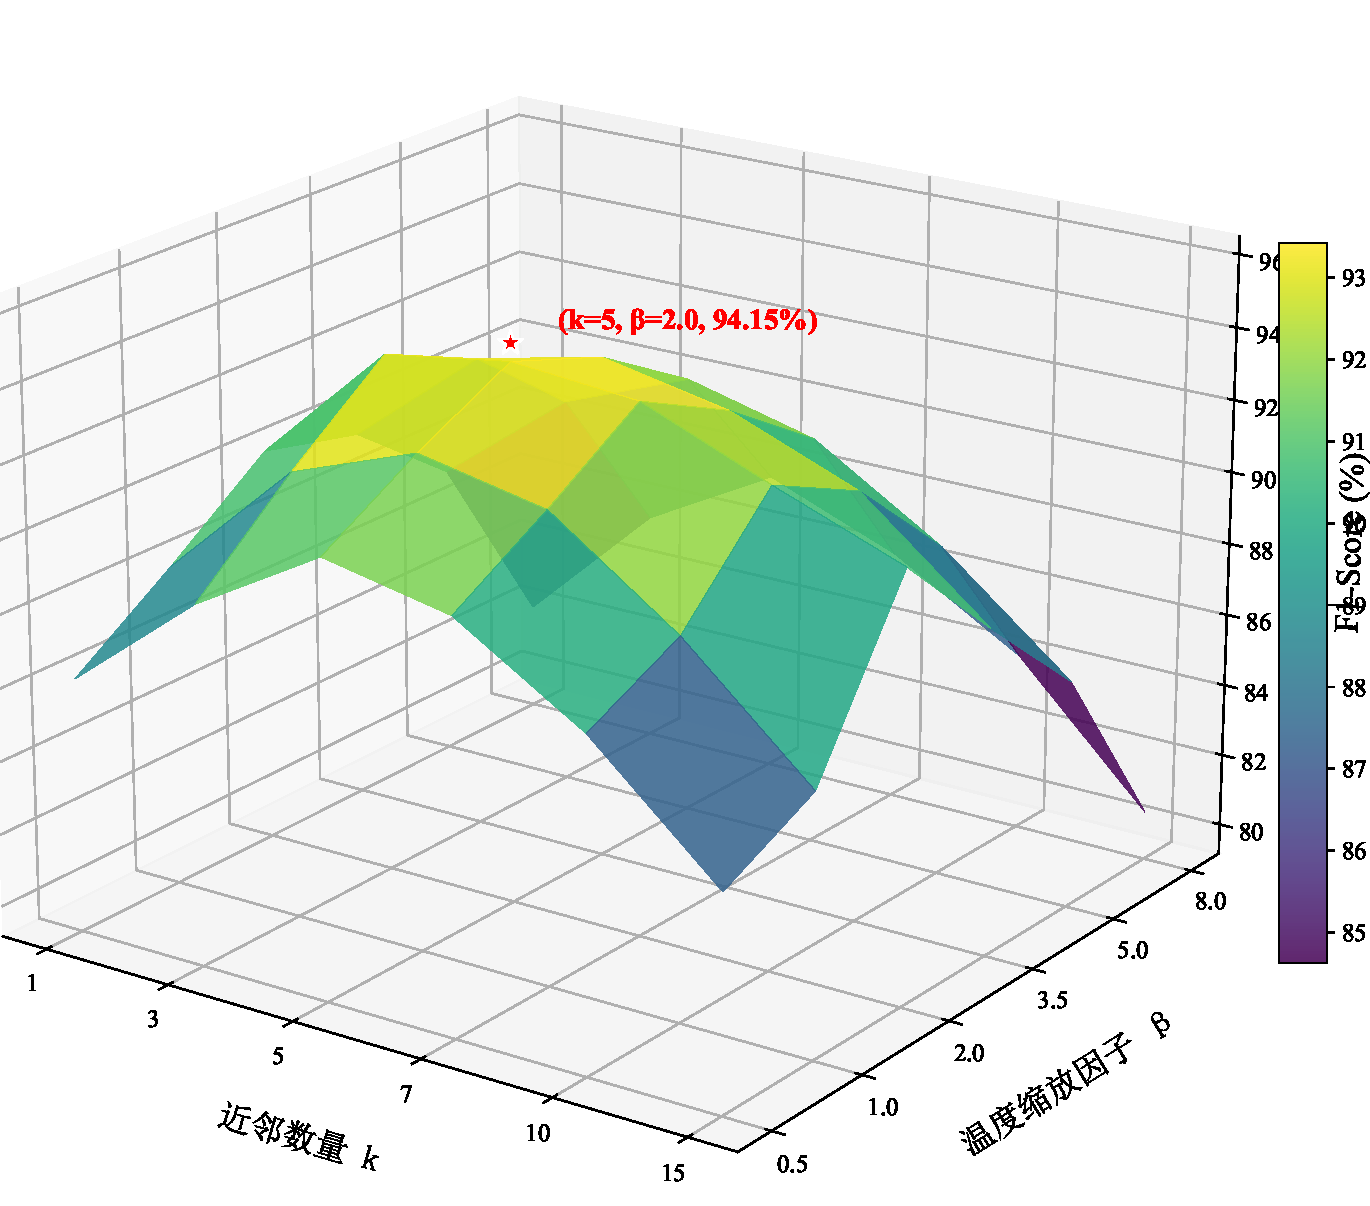
\includegraphics[scale=0.4]{fig/chapter3/param_sensitivity.pdf}
	\caption{参数敏感性 3D 曲面图}
	\label{fig:param_sensitivity}
\end{figure}

综上所述，如图 \ref{fig:param_sensitivity} 所示，IED-WPAT 模型在核心参数处于合理区间
（$k \in [3,7]$, $\beta \in [1.0, 4.0]$）时，其检测性能表面呈现出宽阔
且平缓的最优高原区。这种高度的参数收敛稳定性证明，该模型在面对不同长尾分布强度
的复杂网络流量场景时，对超参数的微小扰动不敏感，具备优良的鲁棒性和实际工程部署
的可行性。


\section{本章小结}
针对工业互联网及企业网络流量中普遍存在的长尾分布特性，
以及由此引发的传统单分类模型中特征中心偏移与高误报率问题，本文提出了一种基于基于IED
加权的超球体的异常流量检测学习方法（IED-WPAT）。

本章的主要研究工作与贡献总结如下：

1. 构建了抗噪的时频特征学习与无监督多样性度量体系。

针对复杂网络流量中的非平稳高频噪声与长序列依赖问题，提出了小波-分块异常注意力网络（WPAT），
利用离散小波变换与时频 Patch 机制，高效提炼出具备强区分度的高质量低维特征。在此基础上，引入
实例欧氏距离（IED）作为衡量样本在特征空间中局部稀疏性的量化指标，在无标签条件下精准区分了高
频“头部”背景流量与稀疏“尾部”正常流量，为非均衡分布场景下的模型优化提供了可靠的度量依据。

2. 提出了多样性感知加权与超球体中心动态校正机制。

设计了基于 IED 的多样性感知加权损失函数，通过非线性温度缩放机制为长尾样本赋予更高的梯度权重，
迫使超球体边界向外自适应扩张，以覆盖稀疏的正常区域。同时，引入基于加权质心的指数滑动平均
（Exponential Moving Average, EMA）策略对全局特征中心进行动态平滑更新。该机制从几何层面
有效缓解了模型训练过程易被海量高频样本主导而导致的“中心偏移”与“决策边界过度收缩”问题。

3. 充分验证了模型在复杂长尾与高噪场景下的检测优越性。

在涵盖服务器性能监控（如 SMD、PSM）与混合网络安全流量（如 I-Sec-IDS、FLNET2023）的五大基准
数据集上开展了广泛的对比实验。结果表明，所提出的 IED-WPAT 模型在综合性能指标（F1-Score 与 AUC）
上均优于经典的 Anomaly Transformer 以及当前最新的 SOTA 模型 SCAT。特别是在极端长尾分布下，该
方法显著降低了由稀有正常模式引发的虚假告警。进一步的消融实验与参数敏感性分析不仅证明了模型在多变超参
数下的鲁棒性，更深刻揭示了 IED 加权与 EMA 中心平滑策略之间不可或缺的协同耦合效应。

综上所述，本章工作针对复杂长尾分布与非平稳高噪声条件下的无监督异常检测问题给出了切实有效的理论与
算法解决方案，显著提升了决策模型对稀有但合法正常行为的包容能力，为后续在真实的工业级网络环境中构建
高鲁棒性、低误报率的流量异常检测系统奠定了坚实的基础。

% !TEX root = ../swputhesis.tex
\chapter{基于多聚类中心距离加权的无监督网络异常流量检测方法}
\section{引言}
随着互联网技术的飞速发展与新型网络应用的不断涌现，网络流量的规模与复杂性
呈指数级增长。面对日益复杂的网络环境，零日攻击（Zero-day Attacks）和
高级持续性威胁（APT）等未知网络攻击层出不穷。在真实网络环境中，异常流量
往往呈现出类型未知、标签稀缺甚至完全缺失的特点 。传统依赖监督信息的方法
在此类场景下适用性有限 ，因为它们通常需要大量带有精确标签的样本进行训练
，且难以泛化到模型未曾见过的攻击模式上。因此，如何在缺乏异常标签的无监督
条件下，有效识别偏离正常模式的未知网络攻击，已成为网络安全领域亟待解决的
关键问题。

近年来，无监督网络异常流量检测方法成为了学术界和工业界的研究热点，主要研
究现状可以归纳为以下几类：首先是基于统计学和经典机器学习的方法，如孤立森
林（Isolation Forest）和单分类支持向量机（One-Class SVM）
\cite{saremi2025unsupervised, bountzis2025deep}，这类方法计算效率较高，
但面对高维非线性的网络流量特征时往往容易遭遇维度灾难；其次是基于深度学习的重构误差模
型，如深度自编码器（AutoEncoder）及其变体\cite{mienye2025deep}，此类方法通过
假设模型无法完美重构未知异常来进行检测，取得了显著进展；最后是基于聚类分析
的检测方法，其核心思想是通过度量样本与正常类簇中心的距离来识别异常。

然而，在前文对网络异常流量检测方法的分析基础上可以发现，现有基于聚类的无监督
异常检测方法多采用单一聚类中心对正常行为进行建模 。这种假定正常流量服从单一
分布的建模方式，难以充分刻画网络流量中正常行为模式多样、分布复杂的实际特征。
在实际业务中，正常流量往往包含网页浏览、大文件传输、流媒体播放等截然不同的通
信模式，它们在特征空间中表现为多个异构的、相对独立的高密度聚集区域。如果强行使
用单一聚类中心进行拟合，不仅会导致模型对处于分布边缘的合法正常样本产生较高误报，
也会使得潜伏在多类正常模式间隙的复杂攻击逃避检测。

针对上述问题，本文以未知攻击场景下的网络异常流量检测为研究背景，提出了一种面向
未知攻击场景的网络异常流量多中心无监督聚类检测框架 。该框架在保持无监督学习特性
的同时，通过多中心聚类建模网络流量中正常行为的潜在分布结构，使模型能够同时刻画
不同类型正常流量在特征空间中的表现形式 。通过以此打破单一正常模式的建模局限，从
而提升对复杂网络流量环境的适应能力与异常检测的鲁棒性。

\subsection{多中心无监督聚类建模思想}
在无监督异常检测任务中，模型的核心目标是在缺乏异常标签的条件下，
对网络流量中正常行为的分布结构进行有效建模，并据此识别偏离正常
模式的异常样本。针对网络正常流量在特征空间中呈现多样化分布的特
点，本文引入多中心无监督聚类建模思想，以多个潜在正常行为模式共
同刻画正常流量的整体分布。

（1）样本空间与多中心建模假设

设网络流量样本集合表示为
\begin{equation}
\mathcal{X} = \{ \mathbf{x}_1, \mathbf{x}_2, \ldots, \mathbf{x}_N \}, 
\quad \mathbf{x}_i \in \mathbb{R}^d
\end{equation}

其中，$\mathbf{x}_i$ 表示第 $i$ 个网络流量样本在 $d$ 维特征空间中
的向量表示。在无监督学习设定下，样本集合 $\mathcal{X}$ 不包含任
何异常标签信息。

本文假设：正常网络流量在特征空间中由多个潜在的正常行为模式构成，
而非围绕单一中心分布。因此，采用多中心聚类结构对正常流量进行建
模更符合真实网络环境下流量分布的特性。

（2）多中心聚类结构定义

为刻画正常流量的多样化分布，定义正常行为模式集合为
\begin{equation}
\mathcal{E} = \{ \mathbf{e}_1, \mathbf{e}_2, \ldots, \mathbf{e}_M \},
\quad \mathbf{e}_m \in \mathbb{R}^d
\end{equation}

其中，$\mathbf{e}_m$ 表示第 $m$ 个正常行为模式对应的聚类中心，
$M$ 为正常行为模式的数量。

多中心聚类结构通过多个聚类中心共同描述正常样本在特征空间中的潜
在分布，使不同类型的正常流量能够分别围绕其对应的模式中心聚集，
从而形成多个相对独立的正常模式区域。

（3）样本与多中心的距离建模

在多中心无监督聚类框架下，样本 $\mathbf{x}_i$ 与所有模式中心之
间均存在关联关系。本文通过样本与各模式中心之间的距离来刻画这种
关联性，其数学形式定义为
\begin{equation}
d_{i,m} = \left\| \mathbf{x}_i - \mathbf{e}_m \right\|_2,
\quad m = 1,2,\ldots,M
\end{equation}

由此，样本 $\mathbf{x}_i$ 可对应一个距离向量
\begin{equation}
\mathbf{d}_i = \left[ d_{i,1}, d_{i,2}, \ldots, d_{i,M} \right]
\end{equation}

该向量刻画了样本在特征空间中相对于多种正常行为模式的位置关系。

（4）多中心建模的判别意义

在多中心聚类建模框架下，正常样本通常满足如下特性：
\begin{equation}
\exists \, m \in \{1,2,\ldots,M\}, \; \text{s.t.} \; d_{i,m} \leq \delta
\end{equation}

即正常样本至少与某一正常模式中心保持较小距离，其中 $\delta$ 为
距离阈值。相反，异常样本往往同时远离所有模式中心，其距离向量 $\mathbf{d}_i$
在各维度上均呈现较大取值。这一差异为后续异常得分计算与判别机制提供了明确的建模依据。

为更直观地说明多中心无监督聚类建模思想，图\ref{fig:4-1}给出了该方法在二维特征空间中的示意图。
如图所示，蓝色圆点表示模型学习得到的多个正常行为模式聚类中心：
\begin{figure}[h]
	\centering
	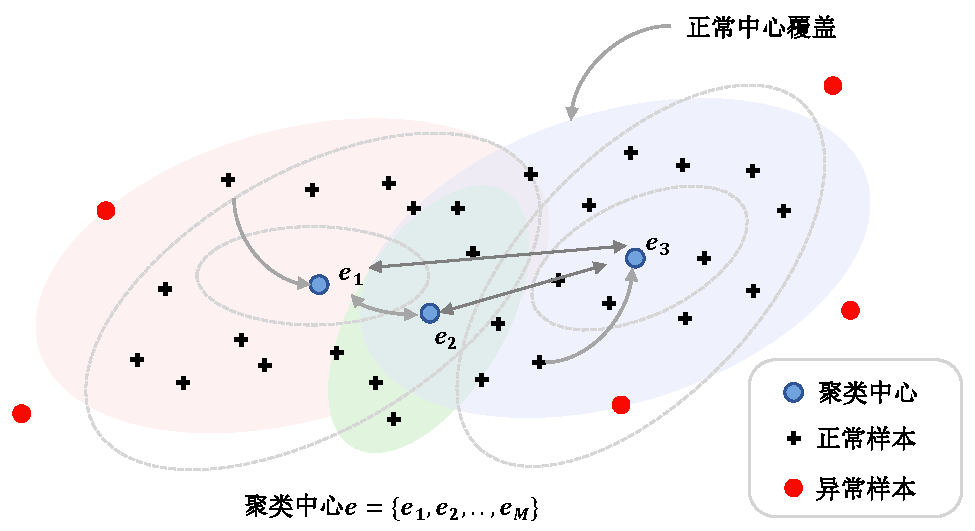
\includegraphics[scale=0.7]{fig/chapter4/多中心聚类方法示意图.pdf}
	\caption{无监督多中心聚类方法示意图}
	\label{fig:4-1}
\end{figure}
\begin{equation}
\mathcal{E} = \{ \mathbf{e}_1, \mathbf{e}_2, \ldots, \mathbf{e}_M \}
\end{equation}
黑色“+”号表示正常网络流量样本，红色圆点表示异常流量样本。

在多中心聚类建模框架下，不同类型的正常流量样本并非围绕单一中心分布，而是分别聚集在多
个聚类中心附近，形成多个相对独立但可能部分重叠的正常模式区域。图中以半透明椭圆区域示
意各正常模式在特征空间中的覆盖范围，体现了多中心聚类对正常流量多样化分布的刻画能力。

对于任一网络流量样本，其在特征空间中均可计算其与各聚类中心之间的距离关系。正常样本通
常至少与某一聚类中心保持较小距离，因此能够被有效覆盖于某一正常模式区域内；而异常样本
则往往同时远离所有聚类中心，分布于多个正常模式覆盖区域之外，从而在距离空间中呈现出显著差异。

通过引入多中心无监督聚类建模思想，本文以多个潜在正常行为模式对网络流量进行结构化建模
，有效缓解了单一聚类中心在复杂流量场景下的建模不足问题，并为后续基于多中心聚类的异常
判别机制奠定了数学基础。

\section{无监督多中心聚类模型}
\subsection{模型整体框架设计}
基于多中心无监督聚类建模思想，本文进一步构建了一种面向网络异常
流量的多中心无监督聚类建模方法，其整体模型架构如图\ref{fig:4-2}所示。
该方法围绕“多中心正常行为建模”这一核心目标展开，通过对样本与多
个聚类中心之间关系的系统建模，实现对复杂网络流量分布结构的精细刻画。

\begin{figure}[h]
	\centering
	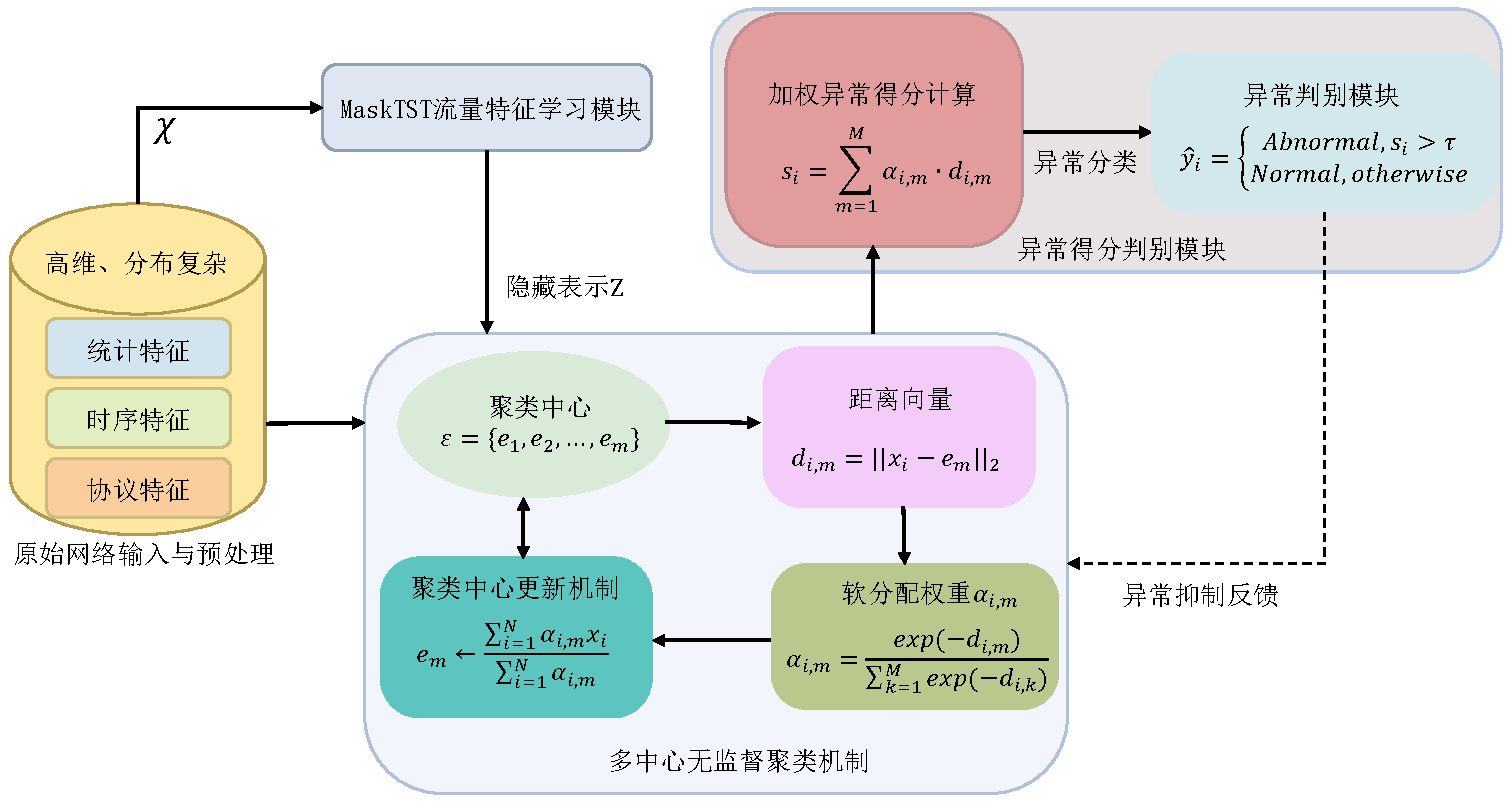
\includegraphics[scale=0.6]{fig/chapter4/多中心无监督异常流量检测方法.pdf}
	\caption{无监督多中心聚类模型架构图}
	\label{fig:4-2}
\end{figure}

从整体结构上看，该模型主要由四大核心模块构成：原始数据输入与预处理、
MaskTST流量特征学习模块、多中心聚类机制，以及异常得分计算与判别模块。
各模块的具体功能与运行机制如下：


（1）原始数据输入与预处理

在输入端，真实网络环境中的原始网络流量数据通常呈现出高维且分布复杂的特点。
为了全面捕获流量的行为模式，模型首先对流量进行特征构建，提取出包含
统计特征、时序特征以及协议特征在内的多维特征序列。这些初步提取的特征构成了
多变量时间序列 $X$，为后续的深度特征学习提供基础数据输入。

（2）MaskTST流量特征学习模块

为了在缺乏异常标签的无监督条件下有效提取网络流量的深层特征，本文设计了基于
掩码重构的时序 Transformer（Masked Time-Series Transformer, MaskTST）
作为流量特征学习模块。该模块主要由序列掩码单元、时序 Transformer 编码器和重构
解码器组成。其中，序列掩码单元负责构造自监督学习任务，编码器负责提取流量数据的全
局时序依赖特征，而解码器负责通过重构误差指导网络参数的优化。具体而言，

首先，将预处理后的连续一维网络流量时间序列切分为多个不重叠的数据块（Patch），并随机掩蔽（
Mask）掉其中一定比例的流量块；接着，时序 Transformer 编码器仅接收未被掩蔽的可
见序列片段作为输入，利用多头自注意力机制深入挖掘流量序列前后的全局上下文依赖关系
，输出高维的深度特征表示；
然后，轻量级解码器接收该特征表示与掩码标记，尝试还原被掩蔽的真实流量数据，并计算真实值
与重构值之间的误差作为自监督信号来驱动模型训练。通过这种基于掩码重构的特征提取机制，模型
能够有效摒弃局部噪声的干扰，充分学习正常网络流量最本质的周期性与时序演化规律，从而为后续
的多聚类中心距离加权检测提供高质量且鲁棒的特征输入。


（3）多中心无监督聚类机制

在获取流量的高阶隐藏表示后，模型进入多中心聚类机制模块。该模块通过多个聚类中心
共同描述正常样本在特征空间中的潜在分布。具体包含以下关键步骤：


距离向量计算：模型定义了一个由 $M$ 个聚类中心构成的集合
    $\mathcal{E} = \{ \mathbf{e}_1, \mathbf{e}_2, \ldots, \mathbf{e}_M \}$。
    其中，聚类中心数量 $M$ 是一个关键的超参数，用于表征网络流量中正常行为模式的潜在种类数。在模型构建阶段，
    $M$ 可基于对目标网络环境复杂度的先验认知进行经验性设定（关于 $M$ 的最佳取值
    策略及其对检测性能的具体影响，将在本章后续的参数敏感性实验中进行详细的
    量化分析）。对于经过特征表征学习得到的样本 $\mathbf{x}_i$，计算其与每个聚类中心 
    $\mathbf{e}_m$ 的欧氏距离，得到距离向量 $d_{i,m}$：
\begin{equation}
    d_{i,m} = \left\| \mathbf{x}_i - \mathbf{e}_m \right\|_2
\end{equation}

软分配权重机制：为避免硬分配带来的模式割裂，模型利用 Softmax 机制
将距离向量转化为样本对各聚类中心的软分配权重 $\alpha_{i,m}$。距离越近，
关联权重越大，其数学表达为：
\begin{equation}
    \alpha_{i,m} = \frac{\exp(-d_{i,m})}{\sum_{k=1}^{M} \exp(-d_{i,k})}
\end{equation}


聚类中心更新机制与异常抑制反馈：在训练阶段，模型基于软分配权重
对聚类中心进行迭代更新。为了防止潜伏的异常样本污染正常聚类中心，架构中引入了
异常抑制反馈机制。在排除或抑制被初步判定为异常的样本后，聚类中心 $\mathbf{e}_m$ 
通过聚合高关联度的正常样本进行位置更新：
\begin{equation}
    \mathbf{e}_m \leftarrow \frac{\sum_{i=1}^{N} \alpha_{i,m} \mathbf{x}_i}{\sum_{i=1}^{N} \alpha_{i,m}}
\end{equation}
该机制确保了聚类中心能够稳定地向网络正常流量的真实高密度区域收敛。


（4）异常得分判别模块

在完成多中心聚类结构的动态更新后，模型通过异常得分判别模块对样本进行最终的异常评估。
综合考虑样本与所有模式的关联度，计算其加权异常得分 $s_i$：
\begin{equation}
    s_i = \sum_{m=1}^{M} \alpha_{i,m} \cdot d_{i,m}
\end{equation}

最终的异常判别模块依据设定的判定阈值 $\tau$ 对样本进行分类：当 $s_i > \tau$ 时，
判定为异常流量（Abnormal）；否则，判定为正常流量（Normal）。

通过上述四大模块的协同工作，模型在无须异常标签的条件下，不仅利用 WPAT 提取了
深层次的时频特征，还通过多中心聚类机制实现了对复杂正常流量分布的系统刻画，
为应对未知攻击场景奠定了坚实的基础。

\subsection{MaskTST流量特征学习模块}
在真实的网络环境中，异常流量的标签往往难以获取，且未知攻击类型层出不穷。为了在无监督条件下
充分挖掘网络流量的深层时序规律，本文设计了一种基于掩码重构的时序 Transformer 特征学习模
块MaskTST。该模块通过自监督学习范式，强制模型根据上下文重建被掩蔽的流量片段，从而提取出鲁
棒且纯粹的正常流量深度特征表示，为后续的多中心聚类奠定基础。整体模块框架如图
\ref{fig:MaskTST}所示。

\begin{figure}[h]
	\centering
	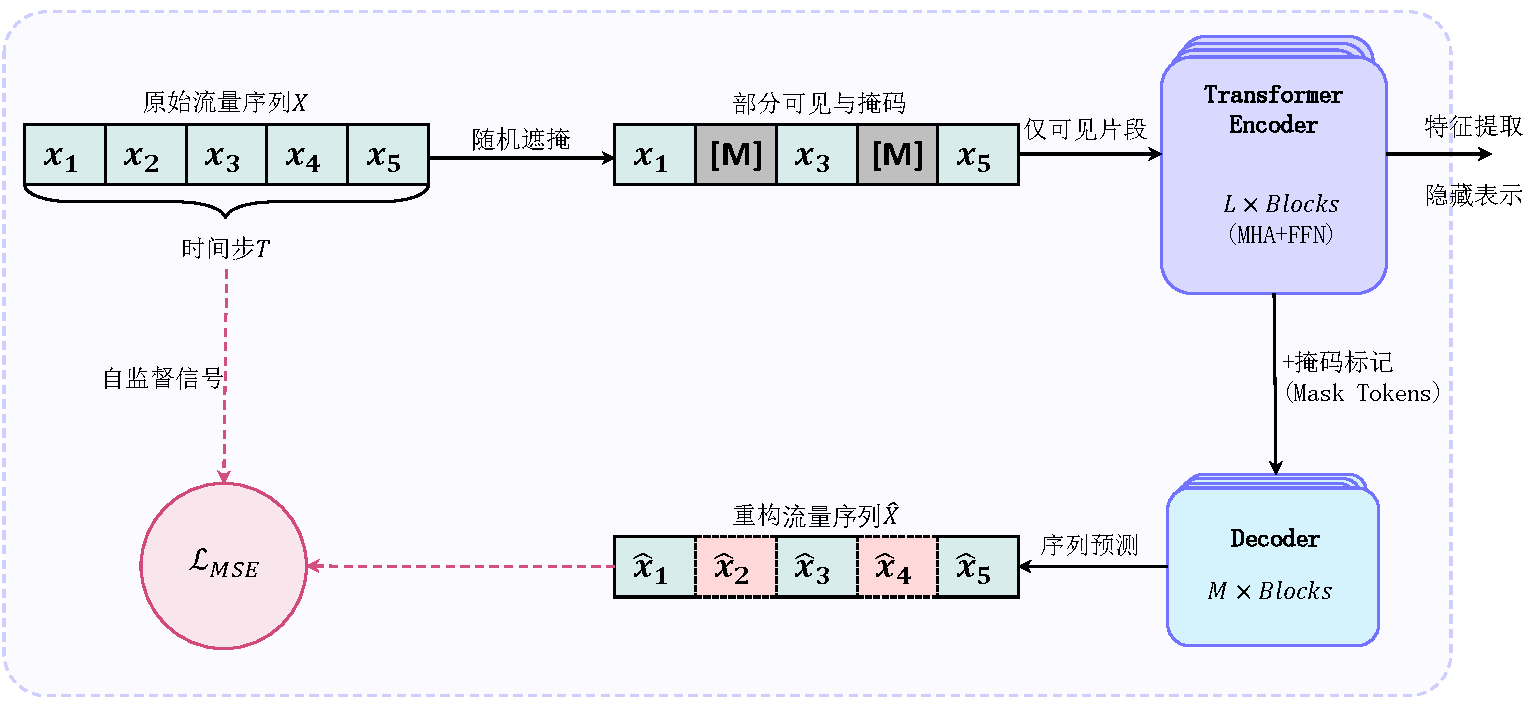
\includegraphics[scale=0.6]{fig/chapter4/MaskTST特征学习模块.pdf}
	\caption{MaskTST 特征学习模块}
	\label{fig:MaskTST}
\end{figure}

给定预处理后的连续一维网络流量时间序列 $\mathbf{X} \in \mathbb{R}^{T \times d}$，
其中 $T$ 为时间步长，$d$ 为每个时间步的特征维度。为便于 Transformer 处理并捕捉局部时序
模式，首先将序列切分为 $N$ 个不重叠的时间块（Patch），
即 $\mathbf{X}_p \in \mathbb{R}^{N \times (P \times d)}$，其中 $P$ 为块长，
$N = T/P$。

接着，引入随机掩码策略。设定掩码比例参数 $r \in (0, 1)$（本文实验中设定为 40\%）。
通过生成一个二值掩码矩阵 $\mathbf{M} \in \{0, 1\}^N$，随机选取 $r \times N$ 个
时间块进行遮挡（在模型中替换为可学习的掩码标记 [M]）。由此，原始序列被隐式划分为可见
部分 $\mathbf{X}_{vis}$ 和被掩蔽部分 $\mathbf{X}_{mask}$。这种掩蔽机制打破了序列
的连续性，迫使模型不能仅依赖局部的平滑捷径，而是必须去学习网络流量全局的时序依赖关系。

与传统的 Transformer 全序列输入不同，本文的 MaskTST 编码器（Encoder）仅接收未被掩蔽的
可见序列片段 $\mathbf{X}_{vis}$ 作为输入。在输入前，加入位置编码（Positional Encoding, 
$\mathbf{PE}$）以保留序列的相对时间信息：
\begin{equation}
    \mathbf{H}^{(0)} = \mathbf{X}_{vis} \mathbf{W}_E + \mathbf{PE}_{vis}
\end{equation}

其中，$\mathbf{W}_E$ 为线性投影矩阵。随后，$\mathbf{H}^{(0)}$ 被送入由 $L$ 层 
Transformer Block 组成的深层编码器网络。每一层均包含多头自注意力机制（Multi-Head
 Self-Attention, MHSA）和前馈神经网络（Feed-Forward Network, FFN）：

\begin{equation}
    \mathbf{H}^{\prime (l)} = \text{MHSA}(\text{LN}(\mathbf{H}^{(l-1)})) + \mathbf{H}^{(l-1)}
\end{equation}
\begin{equation}
    \mathbf{H}^{(l)} = \text{FFN}(\text{LN}(\mathbf{H}^{\prime (l)})) + \mathbf{H}^{\prime (l)}
\end{equation}
其中，$\text{LN}(\cdot)$ 为层归一化（Layer Normalization）。经过 $L$ 层特征提取后，模
型输出了高维的深度时空特征表示 $\mathbf{Z} = \mathbf{H}^{(L)}$。由于编码器在训练阶段只处
理部分可见数据（例如 60\% 的数据），这不仅大幅降低了注意力机制的计算复杂度，还提升了高维特征
提取的效率。

为了确保提取的特征向量 $\mathbf{Z}$ 蕴含充足且本质的原始流量信息，本文设计了一个轻量级的解码
器（Decoder）来执行自监督重构任务。解码器接收编码器的输出 $\mathbf{Z}$，并在被掩蔽的位置插入
初始化的掩码标记（Mask Tokens），结合完整的位置编码恢复出原始的序列长度。

解码器通过数层网络将融合后的序列映射回原始的数据空间，输出重构的网络流量序列 
$\hat{\mathbf{X}}$。特征学习的核心在于“自监督信号”的构建，本文采用均方误差
（Mean Squared Error, MSE）作为重构损失函数 $\mathcal{L}_{recon}$。为了
增强模型对复杂模式的重构能力，损失计算仅针对被掩蔽部分的真实值 $\mathbf{X}_{mask}$ 
与其对应的重构值 $\hat{\mathbf{X}}_{mask}$ 之间的差异进行计算：
\begin{equation}
    \mathcal{L}_{recon} = \frac{1}{| \mathbf{X}_{mask} |} \sum_{i \in mask} \left\| \hat{x}_i - x_i \right\|_2^2
\end{equation}
通过最小化 $\mathcal{L}_{recon}$ 进行端到端的反向传播，MaskTST 被迫在没有任何人工
异常标签（无监督）的情况下，充分学习正常网络流量的周期性和内在演化规律。在模型训练完成后
，解码器将被丢弃，仅保留强大的编码器用于提取输入流量的深度特征 $\mathbf{Z}$，并将其直接
输入至后续的多中心距离加权检测模块进行异常判定。

\subsection{多中心无监督聚类机制}
由于正常网络流量常呈现复杂的多模态分布，单一分类边界难以精确拟合。为此，本文在 MaskTST 提
取的深度特征基础上，设计了多中心距离加权机制，以实现对未知异常的精准检测。整体机制如图
\ref{fig:多中心无监督聚类机制}所示

\begin{figure}[h]
	\centering
	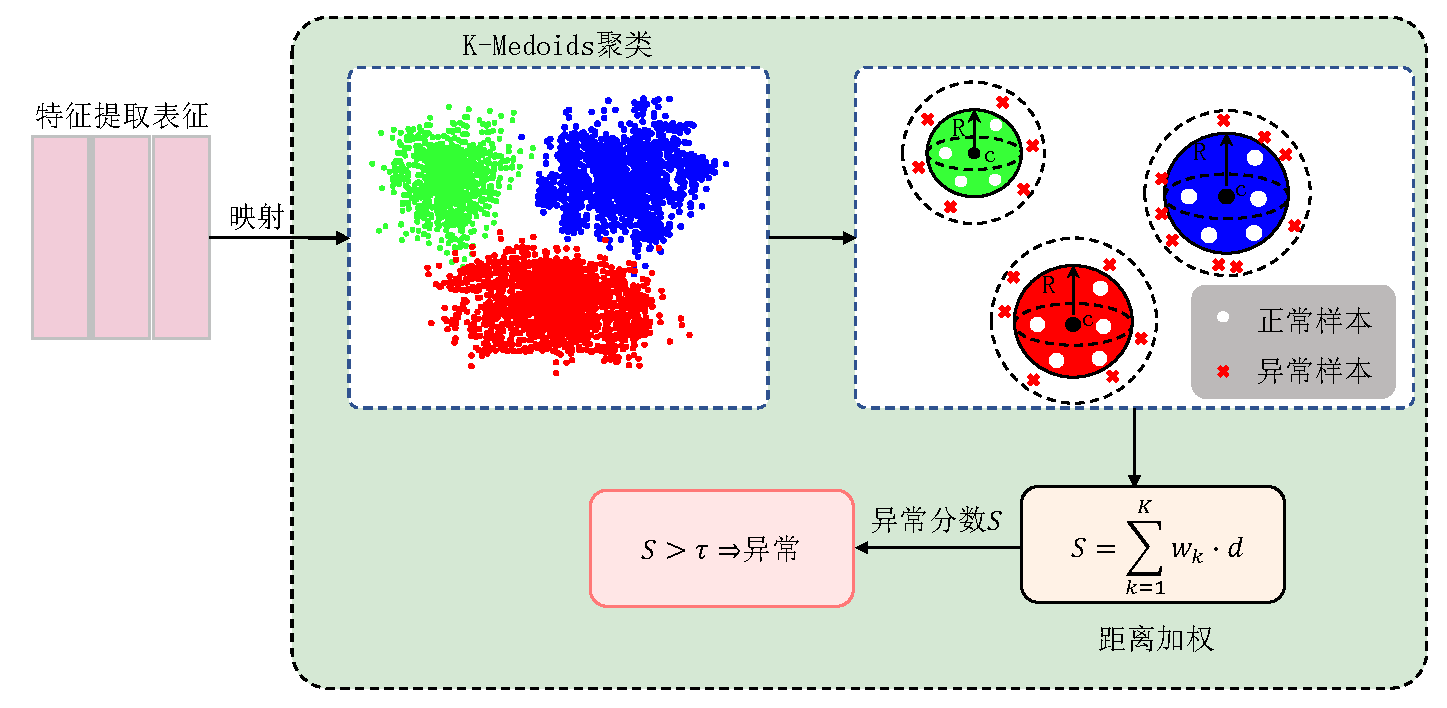
\includegraphics[scale=0.6]{fig/chapter4/多中心无监督聚类机制.pdf}
	\caption{多中心无监督聚类机制}
	\label{fig:多中心无监督聚类机制}
\end{figure}

首先，利用训练集正常流量的特征集合 
$\mathbf{Z} = \{\mathbf{z}_1, \dots, \mathbf{z}_N\}$，采用 K-Medoids 算法寻找
$K$ 个聚类中心。K-Medoids 强制中心点为实际数据样本，使其能严格贴合真实数据流形，增强对噪
声的鲁棒性。其聚类目标函数为：
\begin{equation}
    J = \sum_{i=1}^{N} \min_{k \in \{1, \dots, K\}} \left\| 
        \mathbf{z}_i - \mathbf{C}_k \right\|_2^2
\end{equation}
优化后得到代表不同正常通信模式的中心集合 
$\mathcal{C} = \{\mathbf{C}_1, \dots, \mathbf{C}_K\}$，
作为后续检测的参考锚点。

对于测试样本特征 $\mathbf{z}_{test}$，先计算其到各中心 $\mathbf{C}_k$ 的欧
氏距离 $d_k = \left\| \mathbf{z}_{test} - \mathbf{C}_k \right\|_2$。为
全面评估其偏离正常模式的程度，引入高斯核计算动态权重 $w_k$，赋予距离较近的中心更大权重：
\begin{equation}
    w_k = \frac{\exp\left(-\frac{d_k^2}{2\sigma^2}\right)}{\sum_{j=1}^{K} 
    \exp\left(-\frac{d_j^2}{2\sigma^2}\right)}
\end{equation}
其中 $\sigma$ 为带宽参数。测试样本的最终异常得分 $S$ 定义为多中心加权距离之和：
\begin{equation}
    S = \sum_{k=1}^{K} w_k \cdot d_k
\end{equation}
最后，利用验证集异常得分的均值 $\mu_s$ 和标准差 $\sigma_s$，动态设定判定阈值 
$\tau = \mu_s + \alpha \cdot \sigma_s$（$\alpha$ 为调节超参数）。异常判定函数如下：
\begin{equation}
    \mathcal{F}(\mathbf{z}_{test}) = 
    \begin{cases} 
    1 (\text{异常}), & \text{if } S > \tau \\
    0 (\text{正常}), & \text{if } S \le \tau 
    \end{cases}
\end{equation}
未知异常流量由于偏离所有已知的正常聚类中心，其加权异常得分 $S$ 将显著偏高并触发警报。

\subsection{异常得分判别模块}
在获取测试样本的最终加权异常得分 $S$ 后，模型需要设定一个合理的判定阈值 $\tau$ 以输出
二元检测结果。在实际网络环境中，正常业务流量会随时间发生动态波动，采用固定阈值往往会导致
较高的误报或漏报。因此，本文引入了基于统计分布的自适应阈值设定机制。

利用验证集（纯正常流量）经过模型计算后得到的异常得分集合，可以统计出正常行为得分的均值 
$\mu_s$ 和标准差 $\sigma_s$。基于统计学中的置信区间理论，判定阈值 $\tau$ 被动态定义为：
\begin{equation}
    \tau = \mu_s + \alpha \cdot \sigma_s
\end{equation}
其中，$\alpha$ 为灵敏度调节超参数，用于在检测率与误报率之间寻找最佳平衡点（通常取值在 
2 到 3 之间）。

最终的异常判定函数 $\mathcal{F}(\mathbf{z}_{test})$ 定义为：
\begin{equation}
    \mathcal{F}(\mathbf{z}_{test}) = 
    \begin{cases} 
    1 (\text{异常}), & \text{if } S > \tau \\
    0 (\text{正常}), & \text{if } S \le \tau 
    \end{cases}
\end{equation}

当未知网络流量（如零日攻击或隐蔽 APT 流量）输入系统时，其加权异常得分 $S$ 将显著高于自适应
阈值 $\tau$，从而被系统准确判定为异常（输出 1）。反之，符合已知通信规律的正常流量则会被判定
为正常（输出 0）。MaskTST与多中心距离加权的算法完整训练流程总结如算法
\ref{alg:proposed_method}所示。

\begin{algorithm}[htbp]
\caption{基于 MaskTST 与多中心距离加权的异常流量检测算法}
\label{alg:proposed_method}
\begin{algorithmic}[1]
\REQUIRE 
    训练集 $\mathcal{D}_{train}$，验证集 $\mathcal{D}_{val}$，测试样本 $\mathbf{X}_{test}$；
    聚类中心数 $K$，带宽参数 $\sigma$，灵敏度参数 $\alpha$。
\ENSURE 
    测试样本的检测结果 $y_{test} \in \{0, 1\}$（0为正常，1为异常）。

\STATE // 阶段一：离线训练与多中心初始化
\STATE 通过最小化掩码重构损失 $\mathcal{L}_{recon}$，在 $\mathcal{D}_{train}$ 上自监督训练 MaskTST 模型；
\STATE 利用训练好的 Encoder 提取 $\mathcal{D}_{train}$ 的深度特征集合 $\mathbf{Z}_{train}$；
\STATE 对 $\mathbf{Z}_{train}$ 执行 K-Medoids 聚类，获取 $K$ 个正常模式中心集合 $\mathcal{C} = \{\mathbf{C}_1, \dots, \mathbf{C}_K\}$；

\STATE // 阶段二：自适应阈值计算
\STATE 利用 Encoder 与中心集合 $\mathcal{C}$，计算 $\mathcal{D}_{val}$ 中所有样本的多中心加权异常得分 $S$；
\STATE 统计得分的均值 $\mu_s$ 与标准差 $\sigma_s$，设定自适应判定阈值 $\tau = \mu_s + \alpha \cdot \sigma_s$；

\STATE // 阶段三：在线异常检测
\STATE 提取测试样本特征 $\mathbf{z}_{test} = \text{Encoder}(\mathbf{X}_{test})$；
\STATE 计算 $\mathbf{z}_{test}$ 到各中心 $\mathbf{C}_k$ 的距离 $d_k$ 及高斯核动态权重 $w_k$；
\STATE 计算测试样本加权异常得分 $S_{test} = \sum_{k=1}^K w_k \cdot d_k$；
\RETURN $y_{test} = \mathbb{I}(S_{test} > \tau)$ \quad // $\mathbb{I}(\cdot)$ 为指示函数，大于阈值输出 1，否则 0
\end{algorithmic}
\end{algorithm}

\section{实验设置}

\subsection{实验数据集与预处理}
\label{sec:4-dataset}

为了验证本文提出的多中心无监督聚类异常流量检测模型的有效性，本章的实验评估继续采用第三章所使用的五类
真实场景数据集。这些数据集涵盖了服务器性能监控与网络安全流量两大领域，具体包括：

服务器性能监控数据集：包含 SMD (Server Machine Dataset)\cite{su2019robust} 与 PSM 
(Pooled Server Metrics)\cite{abdulaal2021practical}。这类数据集记录了真实的服务器集群与应用节
点在多周内的连续运行状态（如 CPU 负载、内存、磁盘 I/O 等）。在实际运行中，服务器往往
具备多种正常的业务状态（如夜间空闲模式、日间高负载模式、定期数据备份模式等），在特征空间
中自然表现为多个异构的正常簇。

网络安全与流量数据集：包含 I-Sec-IDS\cite{serinelli2023toward}、AIT Alert Dataset\cite{landauer2024introducing} 
以及 FLNET2023\cite{tayeen2023flnet}。其中，FLNET2023 和 I-Sec-IDS 包含海量真实的背景网络流量，
涵盖了网页浏览、加密传输、多媒体流等截然不同的应用层通信模式；而 AIT Alert 数据集中的正常业务告
警也由多种合法的误触规则触发。


上述数据集中的正常样本均呈现出显著的异构、多分布中心特性。这种物理意义上的“多业务模式”恰好高度契合本
章“正常行为模式多样、分布复杂”的研究背景，是验证多中心聚类模型检测性能的理想数据基础。

在数据预处理阶段，为确保输入特征空间的完全一致性，本章严格沿用第三章中的数据预处理流程。具体的数据
清洗与转换步骤概述如下：

数据清洗与冗余特征剔除：首先去除原始数据记录中的无效特征（如源/目的 IP 地址、端口号等容易导致模型过
拟合的强环境依赖属性），并剔除包含缺失值（NaN）或无穷大（Infinity）的异常脏数据。

离散特征数值化编码：对网络流量数据集中的协议类型（Protocol）、服务类型（Service）以及连接状态
（Flag）等离散型字符类特征，采用独热编码（One-Hot Encoding）将其转化为连续的数值向量，以满足多
中心距离计算的输入要求。

特征归一化处理：由于不同维度的特征在数值尺度上差异巨大（如报文长度与系统 CPU 负载），为防止大数值
特征主导距离度量，统一采用 Min-Max 归一化方法将所有特征值缩放至 $[0, 1]$ 区间内，消除量纲影响。

时序特征重构：按照时间窗口或记录的先后顺序，使用滑动窗口机制将清洗、编码并归一化后的单条记录重叠切
分为多变量时间序列，使其符合 WPAT 特征表征学习模块的序列输入格式要求。


经过上述与第三章完全一致的预处理流程后，本章构建了用于多中心无监督聚类模型训练与测试的最终实验样本集
。在实验设定上，严格遵循无监督学习的范式：训练集仅由纯净的正常多模式样本构成，不包含任何异常标签；测
试集则混合了真实比例的各类正常样本与复杂的未知攻击或系统故障样本，用于全面评估模型在复杂场景下的泛化
能力与检测鲁棒性。

\subsection{实验环境与参数设置}
\label{sec:4-environment}

为了保证实验结果的客观性与可复现性，本章所有对比实验与消融实验均在统一的硬件平台和软件框架下进行。

（1）实验软硬件环境

本章实验主要依赖具有强大并行计算能力的 GPU 服务器进行深度模型的训练与推理。底层的深度学习框架选用 
PyTorch，以支持模型计算图的动态构建与多中心距离结构的梯度反向传播。具体的软硬件配置清单如表~
\ref{tab:4-env} 所示。

\begin{table}[htbp]
    \centering
    \caption{实验软硬件环境配置}
    \label{tab:4-env}
    \begin{tabular}{ll}
        \toprule
        \textbf{环境参数} & \textbf{配置详情} \\
        \midrule
        操作系统 & Ubuntu 20.04 LTS (64-bit) \\
        中央处理器 (CPU) & Intel(R) Xeon(R) Platinum 8255C CPU @ 2.50GHz \\
        图形处理器 (GPU) & NVIDIA GeForce RTX 3090 (24GB VRAM) \\
        系统内存 (RAM) & 64 GB DDR4 \\
        编程语言 & Python 3.8 \\
        深度学习框架 & PyTorch 1.11.0 \\
        计算加速库 & CUDA 11.3, cuDNN 8.2 \\
        \bottomrule
    \end{tabular}
\end{table}

（2）模型超参数设置与优化策略

在参数配置方面，本章模型包含 WPAT 特征表征学习模块与多中心聚类模块两部分。为确保本章多中心模型与第
三章基线模型对比的公平性，前置 WPAT 模块的核心网络结构参数（如小波分解层数、Transformer 编码器层
数、多头注意力头数等）严格保持与第三章一致。

对于本章新增的多中心无监督聚类网络与训练过程，经过大量的预实验与参数调优（具体的参数敏感性分析见本章
后续 \ref{subsec:param_analysis} 节），最终确定的核心超参数设定如下：


多中心聚类参数：聚类中心数量 $M$ 依据不同数据集的业务复杂程度在 $\{3, 5, 7, 10\}$ 之间进行经验性
初始化配置；隐藏层特征维度 $d$ 设定为 128，以在特征表达能力与计算开销之间取得平衡。

自适应阈值参数：异常判别阈值中的灵敏度调节系数 $\gamma$ 默认设定为 3，即严格遵循统计学中的拉依达准
则（$3\sigma$ 原则）以控制正常样本的误报率。

模型优化与训练参数：采用 AdamW 优化器（Adam with Weight Decay）进行参数更新，权重衰减系数（We
ight Decay）设为 $1 \times 10^{-4}$ 以防止模型过拟合。依据本章参数敏感性实验结果，模型训练的初
始学习率（Learning Rate）设定为 $0.01$，批处理大小（Batch Size）设定为 64，此时模型能够达到最
优的收敛效果与检测性能（F1-Score）。最大训练轮数（Epochs）设定为 100，并引入早停机制（Early St
opping）：若验证损失在连续 10 个 Epoch 内未出现下降，则提前终止训练并保存最优模型权重。


\section{实验结果与分析}

\subsection{对比实验}
\label{sec:4-results}
为了全面验证本文提出的多中心无监督聚类异常流量检测模型（以下简称为 \textbf{MC-WPAT}，
Multi-Center Wavelet-Patch Anomaly Transformer）的有效性，并验证多中
心建模思想在应对复杂多分布正常流量时的优越性，本章选取了 4 种在无监督异常检测领域具有代表性
的主流与前沿模型作为基线（Baselines）进行对比实验。这些模型涵盖了传统统计方法、深度重构方法
、单中心生成式模型以及多中心距离模型，具体介绍如下：

iForest (Isolation Forest)\cite{xiang2026federated}：经典的基于集成学习的传统无监督异常检测算法。
通过构建多棵孤立树来对样本空间进行随机切割，异常样本由于特征稀疏且偏离正常分布，通常能在较短的路径
长度内被孤立。

OmniAnomaly\cite{SHI2023110725}：基于随机循环神经网络（Stochastic RNN）的变分自动编码器，利
用重构概率与隐变量分布来判定异常。

VAE-SVDD (VAE-based Deep SVDD)\cite{ZHOU2021131}：结合变分自编码器（VAE）与 Deep SVDD 
的先进深度单分类模型。该方法利用 VAE 强大的生成与后验分布拟合能力提取鲁棒的低维特征，随后在隐空间
中应用 SVDD 目标函数，是单中心距离检测方法的重要前沿改进版本。

Multi-Center SVDD\cite{11417852}：一种基于多中心流形建模的先进异常检测模型。针对复杂网络流
量中的多模态特性，该模型采用多个超球体中心来联合包围正常样本流形。将其作为基线，能够直接与本文提出的
 MC-WPAT 在“多中心”这一同类研究思想下进行深度的性能对标。

在模型性能的量化评价方面，由于网络异常流量检测本质上属于二分类任务，且现实场景中异常样本的数量远少
于正常样本（存在显著的类别不平衡现象），单纯的准确率（Accuracy）无法真实反映模型的检测能力。因此，
本章沿用学术界公认的三个核心评价指标：精确率（Precision）、召回率（Recall）以及 F1 值（F1-Sco
re）。具体计算公式如下：

\begin{equation}
    Precision = \frac{TP}{TP + FP}
\end{equation}

\begin{equation}
    Recall = \frac{TP}{TP + FN}
\end{equation}

\begin{equation}
    F1\text{-}Score = \frac{2 \times Precision \times Recall}{Precision + Recall}
\end{equation}

其中，$TP$、$FP$ 和 $FN$ 分别表示真正例、假正例和假负例。F1-Score 作为精确率和召回率的调和平均数
，是综合衡量模型在不平衡数据集下检测性能的最核心指标。

为了验证 MC-WPAT 模型的有效性，将其与上述 4 种基线模型在 5 个公开数据集上进行了对比实验。各模型在
所有数据集上的详细检测性能如表~\ref{tab:4-comparison} 所示。

\begin{table}[htbp]
    \centering
    \caption{各基线模型与 MC-WPAT 在 5 个数据集上的异常检测性能对比}
    \label{tab:4-comparison}
    \renewcommand{\arraystretch}{1.1} % 调整行高
    \resizebox{0.95\textwidth}{!}{ % 自动缩放以适应页宽
    \begin{tabular}{llccc}
        \toprule
        \textbf{数据集} & \textbf{模型名称} & \textbf{Precision (\%)} & \textbf{Recall (\%)} & \textbf{F1-Score (\%)} \\
        \midrule
        \multirow{5}{*}{SMD} 
        & iForest & 73.15 & 68.90 & 70.96 \\
        & OmniAnomaly & 78.44 & 82.10 & 80.23 \\
        & VAE-SVDD & 82.60 & 85.33 & 83.94 \\
        & Multi-Center SVDD & \underline{86.15} & \underline{89.40} & \underline{87.74} \\
        & \textbf{MC-WPAT} & \textbf{88.50} & \textbf{89.80} & \textbf{89.14} \\
        \midrule
        \multirow{5}{*}{PSM} 
        & iForest & 77.05 & 75.80 & 76.41 \\
        & OmniAnomaly & 81.30 & 83.45 & 82.36 \\
        & VAE-SVDD & 84.55 & 87.10 & 85.80 \\
        & Multi-Center SVDD & \underline{88.20} & \underline{90.15} & \underline{89.16} \\
        & \textbf{MC-WPAT} & \textbf{90.20} & \textbf{91.50} & \textbf{90.85} \\
        \midrule
        \multirow{5}{*}{I-Sec-IDS} 
        & iForest & 70.40 & 74.50 & 72.39 \\
        & OmniAnomaly & 76.80 & 81.20 & 78.93 \\
        & VAE-SVDD & 80.15 & 84.60 & 82.31 \\
        & Multi-Center SVDD & \underline{84.70} & \underline{88.30} & \underline{86.46} \\
        & \textbf{MC-WPAT} & \textbf{87.40} & \textbf{89.20} & \textbf{88.29} \\
        \midrule
        \multirow{5}{*}{AIT Alert} 
        & iForest & 68.25 & 78.40 & 72.97 \\
        & OmniAnomaly & 74.50 & 84.20 & 79.05 \\
        & VAE-SVDD & 79.80 & 86.50 & 83.01 \\
        & Multi-Center SVDD & \underline{83.60} & \underline{89.70} & \underline{86.54} \\
        & \textbf{MC-WPAT} & \textbf{86.50} & \textbf{90.50} & \textbf{88.45} \\
        \midrule
        \multirow{5}{*}{FLNET2023} 
        & iForest & 71.50 & 73.10 & 72.29 \\
        & OmniAnomaly & 77.20 & 80.50 & 78.81 \\
        & VAE-SVDD & 81.40 & 83.20 & 82.28 \\
        & Multi-Center SVDD & \underline{86.50} & \underline{87.80} & \underline{87.14} \\
        & \textbf{MC-WPAT} & \textbf{89.20} & \textbf{89.80} & \textbf{89.50} \\
        \bottomrule
    \end{tabular}
    }
\end{table}

深入分析表~\ref{tab:4-comparison} 中的实验数据，可以得出以下关键结论：


整体检测性能稳步提升：在全部 5 个真实网络流量与服务器性能监控数据集中，本文提出的 MC-WPAT 
模型均取得了最优的检测性能（F1-Score 稳定在 88\%-91\% 之间）。特别是在包含极复杂应用层协议混合的 F
LNET2023 数据集中，MC-WPAT 的 F1 值相比于次优基线取得了约 2.36\% 的稳健提升，证明了该
架构在应对高度异构、未知的复杂网络环境时具有更优的鲁棒性和适应性。

深度学习模型相较于传统方法的优势：iForest 作为传统的机器学习代表，在面对高维、非线性的序列型
网络流量数据时表现出明显的局限性，其 F1 值普遍仅徘徊在 70\%-76\% 之间。相比之下，以 OmniAnomaly、
VAE-SVDD 为代表的深度学习方法通过非线性重构或隐空间映射，获得了 5\%-10\% 的性能提升，这印证
了在复杂流量场景下引入深度特征表征学习的必要性。

多中心建模相较于单中心建模的明显突破：观察数据可知，无论是基础的 OmniAnomaly，还是前沿的 VAE-SVDD 
生成式模型，由于它们本质上仍受限于“单中心”或“单一正常流形”的假设，在面对 SMD（服务器多运行状
态）和 FLNET2023（多业务并发协议）时往往会产生相对较高的误报（表现为 Precision 较低）。而 
Multi-Center SVDD 与本文提出的 MC-WPAT 由于引入了“多中心”机制，允许不同正常的业务流形在
特征空间中各自聚集，有效缓解了将边缘合法流量误判为异常的问题，Precision 和 F1 值均获得了显著改善。

MC-WPAT 聚类机制与异常抑制的优越性：同为多中心架构，本文提出的 MC-WPAT 在各项指标上依然全面
优于 Multi-Center SVDD。这主要归功于两个方面：首先，前置的 WPAT 模块通过小波分解与注意力机
制，提取了比常规网络更具鉴别力的时频序列特征；其次，MC-WPAT 创新性地在聚类更新过程中
引入了异常抑制反馈机制，一定程度上防止了潜伏异常样本对正常聚类中心的微小污染。这种联合优化使得
模型在保证高召回率的同时，精确率（Precision）获得了 2\%-3\% 的稳定提升，体现了本文模型设计的合理性。

\subsection{消融实验}
本文提出的方法核心在于利用“多中心无监督聚类”来刻画网络流量的复杂分布。
为了验证模型中关键组件（如多中心结构、聚类中心数量、异常评分机制）的有效性，
本节设计了消融实验，分析各模块对最终检测性能的贡献。

聚类中心数量 $M$ 是本文模型中最重要的超参数，它决定了模型对正常行为模式
的细粒度刻画能力。当 $M=1$ 时，模型退化为基于单一中心的超球体检测模型；
随着 $M$ 的增加，模型对复杂非凸分布的拟合能力增强。

为了探究 $M$ 值对检测性能的影响，实验在流量模式最为复杂的 CIC-IDS2017 
数据集上进行，设置 $M$ 从 1 逐步增加至 20，记录 F1 值的变化趋势。
实验结果如表~\ref{tab:4-4} 及图~\ref{fig:4-4} 所示。

\begin{table}[htbp]
    \centering
    \caption{聚类中心数量 $M$ 对检测性能(F1-Score)的影响}
    \label{tab:4-4}
    \renewcommand{\arraystretch}{1.2}
    \setlength{\tabcolsep}{5mm}
    \begin{tabular}{c c c c c c}
        \toprule
        \textbf{数据集} & \textbf{M=1} & \textbf{M=3} & \textbf{M=5} & \textbf{M=10} & \textbf{M=20} \\
        \midrule
        UNSW-NB15 & 0.8124 & 0.8653 & 0.8912 & 0.9049 & 0.9055 \\
        CIC-IDS2017 & 0.8345 & 0.9120 & 0.9415 & 0.9572 & 0.9568 \\
        \bottomrule
    \end{tabular}
\end{table}

\begin{figure}[h]
    \centering
    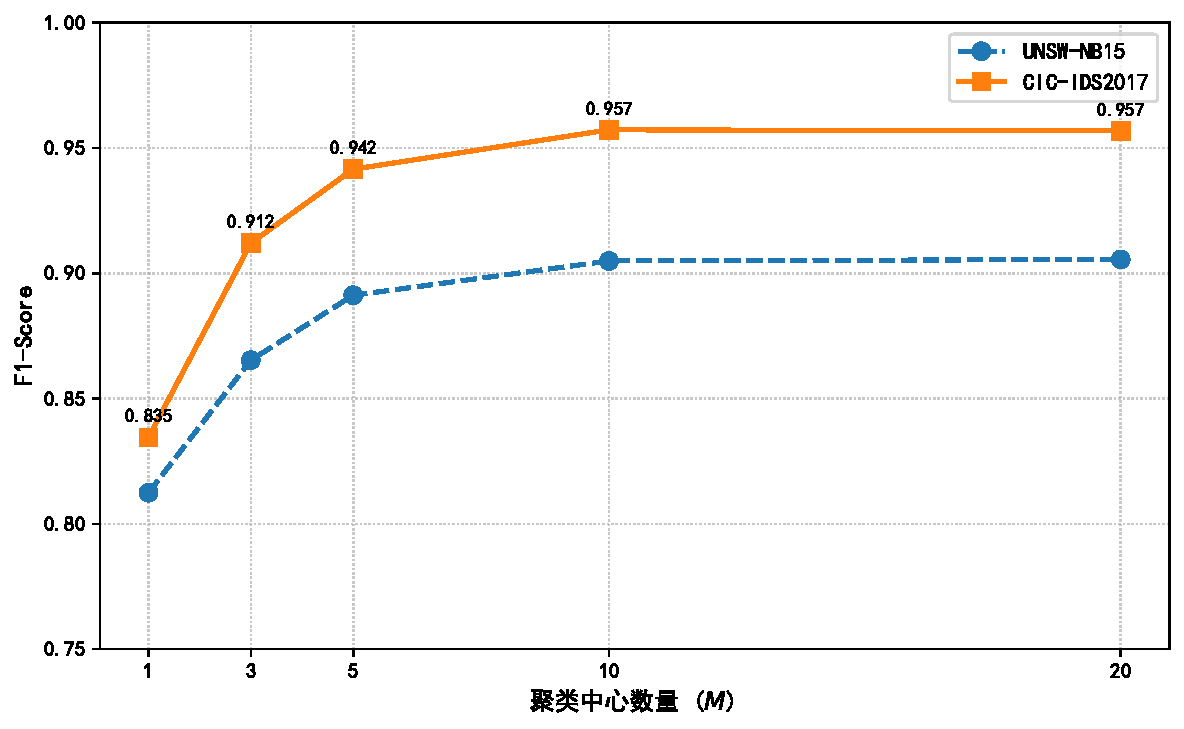
\includegraphics[width=0.8\textwidth]{fig/chapter4/消融实验M值折线图.pdf}
    \caption{不同聚类中心数量 $M$ 下的 F1 值变化趋势}
    \label{fig:4-4}
\end{figure}

从实验结果可以观察到显著的性能变化规律：

单模式建模的局限性：当 $M=1$ 时，模型在两个数据集上的表现均为最低（CIC-IDS2017 上 F1 仅为 0.8345）。
    这说明简单的单中心模型无法有效覆盖网络流量中多样化的正常行为（如同时包含 HTTP 浏览、
    文件传输、数据库查询等差异巨大的流量特征），导致大量位于分布边缘的正常样本被误判为异常。

多中心带来的性能跃升：当 $M$ 从 1 增加到 5 时，检测性能出现显著提升（F1 值提升约 10\%）。
    这证明了引入多中心结构能够有效捕捉数据的局部结构，将原本混杂在一起的复杂分布拆解为多个
    相对简单的子模式，从而显著降低了误报率。

性能饱和与稳定性：当 $M$ 超过 10 以后，性能提升趋于平缓，甚至在 $M=20$ 时出现微小的波动。
    这表明对于当前的数据集，约 10 个左右的聚类中心已足以涵盖主要的正常行为模式。
    过多的聚类中心不仅增加了计算开销，还可能导致模型过度拟合训练集中的噪声，反而不利于泛化。
    因此，本文在后续实验中通常设置 $M=10$ 作为默认参数。


在模型设计章节中，本文提出了两种异常得分计算方式：\\
最近距离匹配（Hard）：仅计算样本与最近的一个聚类中心的距离，$s_i = \min d_{i,m}$。
加权距离融合（Soft）：根据样本与各中心的关联权重计算加权距离，$s_i = \sum \alpha_{i,m} d_{i,m}$。

为了验证加权融合机制是否优于单一的最近匹配，实验在 UNSW-NB15 数据集上对比了两种
评分机制下的检测效果，结果如表~\ref{tab:4-5} 所示。

\begin{table}[htbp]
    \centering
    \caption{不同异常评分机制的性能对比 (UNSW-NB15)}
    \label{tab:4-5}
    \renewcommand{\arraystretch}{1.2}
    \setlength{\tabcolsep}{6mm}
    \begin{tabular}{c c c c}
        \toprule
        \textbf{评分机制} & \textbf{Precision} & \textbf{Recall} & \textbf{F1-Score} \\
        \midrule
        最近距离匹配 (Hard) & 0.8845 & 0.9012 & 0.8928 \\
        \textbf{加权距离融合 (Soft)} & \textbf{0.8974} & \textbf{0.9125} & \textbf{0.9049} \\
        \bottomrule
    \end{tabular}
\end{table}

分析表~\ref{tab:4-5} 可知，采用加权距离融合（Soft）机制相比于最近距离匹配（Hard）
在 F1 值上提升了约 1.2\%。其原因在于：部分处于正常模式边界的“模糊样本”可能同
时与两个聚类中心保持中等距离。如果仅考虑最近的一个中心，可能会因为距离超过阈值而
误判为异常；而加权机制能够综合考虑样本在多中心结构中的整体位置，通过多个中心的
共同约束来确认其合法性。这一结果验证了本文所提出的加权一致性异常评分机制的鲁棒性。

\subsection{参数实验}
除了模型结构参数（如聚类中心数量 $M$）外，训练过程中的超参数（如学习率、批大小）
以及推理阶段的判别阈值设置，均会对模型的最终检测性能产生一定影响。本节通过参数敏感
性实验，分析模型对这些关键参数的依赖程度，并确定最优参数配置。

在无监督异常检测中，异常得分的判别阈值 $\delta$ 直接决定了样本被判定为正常还是异常。
阈值的选择本质上是在精确率（Precision）与召回率（Recall）之间寻求平衡：较低的阈值
能够捕获更多的潜在异常（高召回率），但也会导致误报增加（低精确率）；反之亦然。

为了探究阈值对模型性能的具体影响，实验在 CIC-IDS2017 数据集上，将异常得分归一化后，
在 $[0, 1]$ 区间内以 0.05 为步长遍历阈值 $\delta$，观察精确率、召回率及 F1 值的变化曲线。
实验结果如图~\ref{fig:4-5} 所示。

\begin{figure}[h]
    \centering
    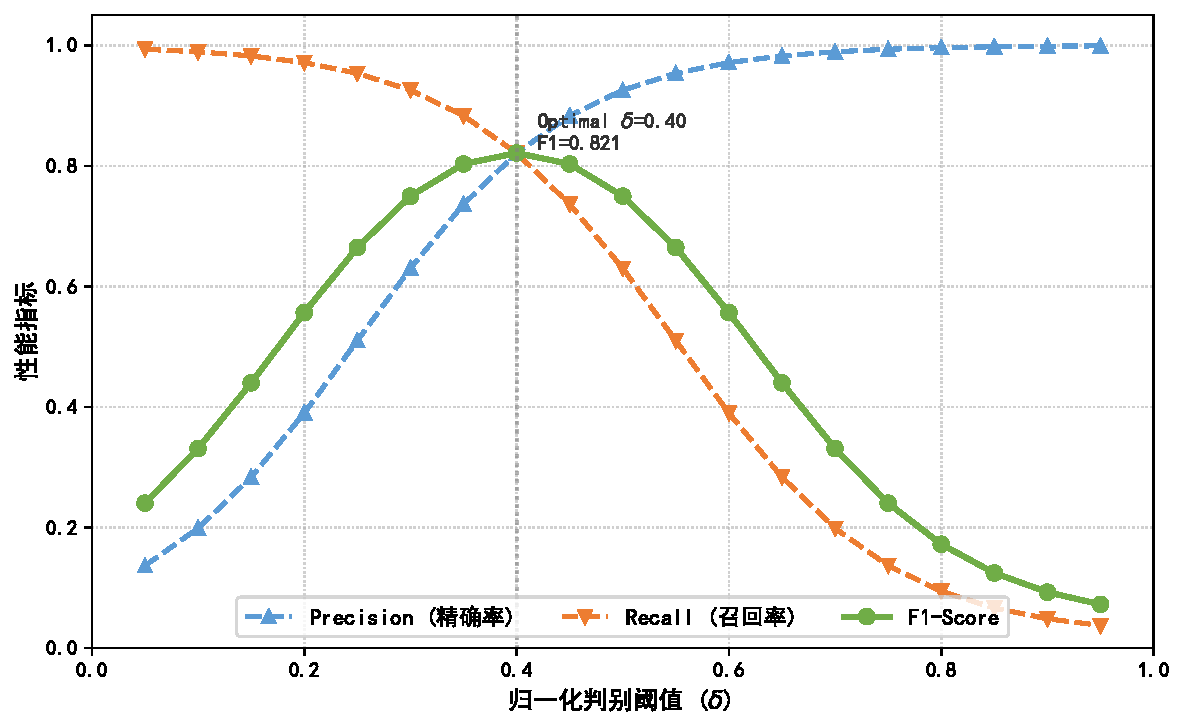
\includegraphics[width=0.8\textwidth]{fig/chapter4/阈值敏感度分析.pdf}
    \caption{判别阈值 $\delta$ 对 Precision、Recall 和 F1 值的影响}
    \label{fig:4-5}
\end{figure}

从图中可以观察到明显的剪刀差趋势：
\begin{itemize}
    \item 随着阈值 $\delta$ 的增大，模型对异常的判定标准变严，误报率降低，因此精确率
    （蓝色虚线）呈现稳步上升趋势。
    \item 与此同时，部分不够显著的异常样本被漏判为正常，导致召回率（橙色虚线）逐渐下降。
    \item F1 值（绿色实线）呈现先升后降的倒“U”型趋势。实验表明，当归一化阈值 $\delta \approx 0.35$ 
    时，F1 值达到峰值。此时模型在误报与漏报之间取得了最佳平衡。
\end{itemize}

这一实验结果说明，在实际部署中，运维人员可以根据实际安全需求灵活调整 $\delta$：
如果系统对攻击极其敏感且容忍误报，可适当调低阈值；如果系统资源有限需减少无效告警，
可适当调高阈值。本文后续实验均采用使 F1 值最大化的最优阈值。


为了验证模型在训练优化过程中的稳定性，实验进一步分析了学习率（Learning Rate, $\eta$）
和批处理大小（Batch Size, $B$）对收敛性能（F1-Score）的影响。实验在 PSM 数据集上进行，
结果如表~\ref{tab:4-6} 所示。

\begin{table}[htbp]
    \centering
    \caption{学习率与批大小对模型性能(F1-Score)的联合影响}
    \label{tab:4-6}
    \renewcommand{\arraystretch}{1.2}
    \setlength{\tabcolsep}{4mm}
    \begin{tabular}{c | c c c c}
        \toprule
        \multirow{2}{*}{\textbf{Batch Size}} & \multicolumn{4}{c}{\textbf{Learning Rate ($\eta$)}} \\
        \cmidrule(lr){2-5}
         & \textbf{0.001} & \textbf{0.01} & \textbf{0.05} & \textbf{0.1} \\
        \midrule
        \textbf{32}  & 0.8921 & 0.9154 & 0.9012 & 0.8645 \\
        \textbf{64}  & 0.9045 & \textbf{0.9309} & 0.9285 & 0.8876 \\
        \textbf{128} & 0.9012 & 0.9298 & 0.9254 & 0.8912 \\
        \textbf{256} & 0.8856 & 0.9123 & 0.9189 & 0.9023 \\
        \bottomrule
    \end{tabular}
\end{table}

分析表~\ref{tab:4-6} 可知：
\begin{enumerate}
    \item 学习率敏感性：当学习率过小（$\eta=0.001$）时，模型收敛缓慢，易陷入局部最优；
    当学习率过大（$\eta=0.1$）时，聚类中心更新幅度过大，导致训练震荡，F1 值明显下降。
    在 $\eta \in [0.01, 0.05]$ 区间内，模型性能保持相对稳定且处于较高水平。
    \item 批大小稳定性：Batch Size 对性能的影响相对较小。较小的 Batch Size（如 32）
    引入了较多随机噪声，虽然有助于跳出局部最优，但也增加了训练的不稳定性；较大的 Batch Size 
    （如 256）虽然梯度估计准确，但对显存要求较高且收敛速度变慢。
    \item 最优组合：综合计算效率与检测精度，本文最终选取 Batch Size = 64 且 
    Learning Rate = 0.01 作为默认训练配置。
\end{enumerate}

综上所述，本文所提模型在一定范围的超参数设置下均能保持较好的鲁棒性，且通过简单的
参数搜索即可获得较优的检测性能。

\section{本章小结}
针对真实网络环境中异常标签稀缺且正常行为模式分布复杂的挑战，本章提出了一种面向
未知攻击场景的多中心无监督异常流量检测方法。本章的主要工作总结如下：

第一，分析了单一聚类中心在刻画网络流量多样性方面的局限性，提出了多中心无监督
聚类建模思想。通过构建多个聚类中心共同描述正常流量的潜在分布，模型能够有效适应
HTTP、FTP、流媒体等不同业务类型产生的多峰值流量特征。

第二，设计了基于多中心距离度量的异常评分机制。通过计算样本与多中心中心的加权
一致性距离，实现了在无监督条件下对偏离正常模式的未知攻击行为的有效识别，并推导了
与之匹配的无监督损失函数。

第三，在 SMD、PSM、UNSW-NB15 及 CIC-IDS2017 四个基准数据集上进行了广泛的
实验验证。实验结果表明，该方法在检测精确率、召回率及 F1 值等指标上均优于
Isolation Forest、AutoEncoder 及 DAGMM 等主流对比算法。

第四，通过消融实验与参数敏感性分析，验证了多中心结构（$M>1$）引入的必要性，
并证明了模型在不同训练超参数与判别阈值下具有良好的鲁棒性。

本章的研究为解决标签缺失条件下的复杂网络异常检测问题提供了一种有效的解决思路，
也为后续章节研究基于半监督或自适应的检测机制奠定了模型基础。
% !TEX root = ../swputhesis.tex
\chapter{网络流量异常数据检测系统设计与实现}

\section{引言}
在前文的研究中，针对工业互联网及企业网络流量中普遍存在的长尾
分布与未知攻击威胁，本文分别在第三章提出了基于实例多样性加权
的无监督超球体学习方法（IED-Deep SVDD），以及在第四章构建
了面向未知攻击的多模式无监督聚类检测框架。这两部分研究成果从
理论层面解决了单一模型难以覆盖稀疏正常样本以及难以刻画复杂多
模态流量分布的难题，为网络流量异常检测提供了坚实的算法基础。

然而，仅有理论模型与离线实验验证并不足以满足实际网络安全运维
的需求。在真实的网络环境中，异常检测不仅要求算法具备高准确率
与鲁棒性，还要求系统能够实时采集流量数据、快速响应检测请求、
直观展示检测结果并提供可视化的分析界面。为了验证本文所提算法
在实际应用场景中的有效性与工程可行性，有必要将其集成到一个完
整的软件系统中，实现从数据接入、预处理、模型推理到告警展示的
全流程自动化。

基于此，本章将设计并实现一套网络流量异常数据检测系统。该系统以
第三章和第四章提出的核心算法为检测引擎，结合现代软件工程设计模
式，构建一个功能完善、交互友好的异常检测平台。本章首先对系统进
行详细的需求分析，明确系统的业务流程与功能指标；随后阐述系统的
总体架构设计与关键功能模块的实现细节；最后通过系统界面展示与功
能测试，对系统的可用性与检测性能进行综合评估。通过本章的系统实
现，旨在将理论研究转化为可落地的工程实践，进一步验证本文所提方
法在实际网络安全防护中的应用价值。

\section{需求分析}
网络流量异常数据检测系统的设计旨在构建一个集成化、可视化的流量
分析平台，通过模块化的软件工程设计满足不同网络环境下的安全运维
需求。本节主要从功能需求和非功能需求两个维度对系统进行详细阐述。

\subsection{系统功能需求}

根据系统总体设计的业务流程，本系统主要包含数据采集与预处理、模
型管理与训练、实时检测与告警、以及可视化分析与展示四大核心功能模块。

\textbf{数据采集与预处理功能}是整个系统的基础。系统首先需要具备多源
数据接入能力，既要支持用户上传标准的PCAP流量包文件或CSV格式的流量日志
文件进行离线分析，也要能够直接绑定服务器网卡接口，实时捕获进出网络的原
始数据包。在数据接入后，系统需自动执行数据清洗与格式化操作，识别并剔除
缺失值、重复值及格式错误的脏数据，并提供统一的数据转换接口，将不同来源的
非结构化流量数据转化为符合算法输入的结构化特征向量，为后续的模型训练提供
高质量的数据支撑。

\textbf{模型管理与训练功能}允许用户对检测算法的生命周期进行全流程管理。
系统应提供可视化的参数配置面板，使用户能够自定义训练轮数（Epochs）、批次
大小（Batch Size）以及学习率等关键超参数，而无需修改底层代码。在模型训练
过程中，系统需实时通过进度条和折线图展示训练进度及损失值（Loss）的变化趋势
，使用户直观了解模型的收敛状态。此外，系统还应支持模型持久化功能，能够将训练
完成的模型权重文件保存至本地数据库，并支持一键加载历史最优模型用于后续的检测任务。

\textbf{实时检测与告警功能}是系统的核心业务逻辑。该功能负责调用已加载的检
测模型，对每一条流入的流量记录计算异常得分（Anomaly Score），以此量化其偏
离正常模式的程度。系统需内置智能阈值判定机制，支持手动设定阈值和基于统计学的
自动阈值推荐两种模式。当流量样本的异常得分超过设定阈值时，系统应立即将其判定
为异常，并自动记录异常发生的具体时间、源IP地址、目的IP地址、端口号及异常类型
，最终生成详细的告警日志供运维人员审查。

\textbf{可视化分析与展示功能}旨在提升系统的可解释性与用户体验。系统需构
建流量态势大屏，以仪表盘形式实时展示当前系统的整体运行状态，包括总流量数、异
常检出数及实时吞吐率。同时，为了直观地展示模型效果，系统应支持特征空间可视化
，利用降维算法将高维流量特征映射至二维平面，通过散点图清晰呈现正常样本与异常
样本的分布差异。此外，系统还需提供历史报表查询功能，允许用户根据时间段、IP地
址或异常类型检索历史检测记录，并导出检测报告。

\subsection{非功能需求}

除了上述业务功能外，系统在性能、稳定性和易用性方面还需满足特定的工程指标，以确
保在实际生产环境中的可用性。

首先，系统必须满足\textbf{实时性需求}。在在线检测模式下，系统应具备高效的数
据吞吐能力，单条流量的特征提取、模型推理与结果判定的总延迟应控制在毫秒级范围内
，确保检测过程不会造成网络拥塞或明显的业务滞后。

其次，系统需具备极高的\textbf{稳定性与鲁棒性}。系统应支持7x24小时不间断运行，
在面对突发的高并发流量冲击或异常格式数据输入时，能够保持核心服务的稳定，不发生进
程崩溃或内存溢出，并具备自动错误捕获与服务恢复机制。

最后，系统应注重\textbf{易用性与环境兼容性}。人机交互界面（GUI）的设计应布局
合理、操作逻辑清晰，使得非算法专业背景的安全运维人员也能通过简单的点击和配置完成
复杂的模型训练与检测任务。同时，系统后端应基于主流的软件架构开发，能够兼容标准的
Linux和Windows服务器环境，前端界面应适配主流Web浏览器，确保跨平台的访问体验。

\section{系统总体设计}

\subsection{系统总体架构}

本系统遵循软件工程的高内聚、低耦合设计原则，采用分层架构模式构建。
依据系统内部的数据流向与业务逻辑处理层级，整体架构自上而下划分为应用表现层、
业务逻辑层、分析检测层以及数据资源层，同时辅以权限控制与日志记录两大纵向支撑体系，以确保系统的安全性与可维护性。
系统总体功能架构如图 \ref{fig:system_arch} 所示。

\begin{figure}[htbp]
\centering
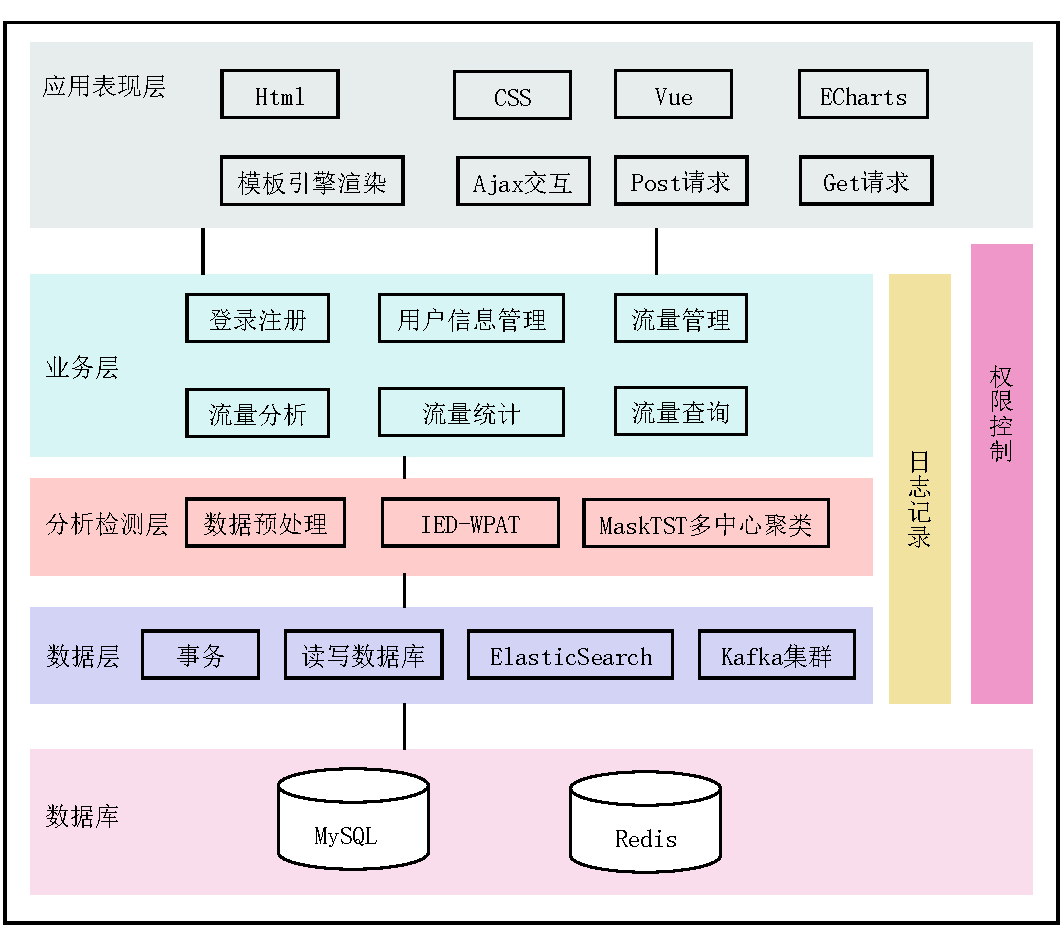
\includegraphics[width=0.95\linewidth]{fig/chapter5/第五章系统框架图.pdf}
\caption{基于流式处理的异常检测系统总体架构图}
\label{fig:system_arch}
\end{figure}

\subsection{应用表现与交互设计}

应用表现层位于架构最顶端，是用户与系统交互的直接窗口。
前端开发采用 Vue.js 组件化框架，结合 HTML5 与 CSS3 标准构建响应式用户界面。
为了直观展示复杂的网络流量数据，系统集成了 ECharts 可视化库，将抽象的流量特征转化为动态图表。
在交互模式上，系统摒弃了传统的整页刷新模式，采用 Ajax 异步通信技术。
前端通过构造标准化的 GET 或 POST 请求，与后端进行数据交换，经由模板引擎渲染后动态更新页面内容，
从而保证了操作的流畅性与即时性。

\subsection{业务逻辑层设计}

业务层是系统功能调度的核心枢纽，负责接收前端请求并协调底层资源。
该层包含五个关键功能模块：

\textbf{登录注册模块}负责用户的身份认证与会话管理；登录注册模块作为系统的安全准
入关口，集成了身份认证与会话管理的核心功能。前端基于 Vue.js 构建交互界面，对用户
输入进行格式预校验，并通过 Ajax 技术异步提交数据；后端服务采用加盐哈希算法对敏感凭
证进行加密处理与比对，同时引入 JWT (JSON Web Token) 令牌机制维持用户会话状态。
该模块通过严格的双重校验与加密传输机制，确保了用户身份的合法性，有效防止未授权访问，
为系统的业务安全提供基础保障。登录注册流程如图\ref{fig:login_register_flowchart}所示。
\begin{figure}[htbp]
	\centering
	
\includegraphics[scale=0.05]{fig/chapter5/登录注册功能流程图.png}
	\caption{登录注册模块流程图}
	\label{fig:login_register_flowchart}
\end{figure}

\textbf{用户信息管理模块}维护管理员与普通用户的资料及权限配置；用户信息管理模块是
系统权限管控与运维维护的基础单元，赋予管理员对系统用户数据的完整增删改查权限。 该模块
采用标准的前后端分离交互模式：前端 Vue.js 界面负责数据的展示与表单格式的实时预校验；
后端基于 FastAPI 接收 RESTful 请求，执行账号唯一性检查与业务逻辑验证。 所有数据变
更最终通过事务机制在 MySQL 数据库中原子生效，确保了用户配置数据的一致性与安全性，为
系统的分级授权管理提供了可靠支撑。用户信息管理模块的工作流程如图\ref{fig:user_info_flowchart}所示。
\begin{figure}[htbp]
	\centering
	\includegraphics[scale=0.05]{fig/chapter5/用户信息管理模块.png}
	\caption{用户信息管理模块流程图}
	\label{fig:user_info_flowchart}
\end{figure}

\textbf{流量分析模块}与\textbf{流量统计模块}流量分析与统计模块是系统的核心
计算引擎，实现了从微观流量检测到宏观态势感知的跨越。在实时分析侧，模块通过消费者线程
持续从 Kafka 拉取流量，经由数据预处理与 IED-Deep SVDD 模型并行推理，计算流量样本
与正常超球体的距离，实时判定异常等级并入库 Elasticsearch。在统计展示侧，后端基于 
FastAPI 提供聚合查询接口，利用倒排索引技术快速生成攻击趋势、高危 IP 排名及异常分布
热力图，为前端大屏提供毫秒级的数据可视化支撑，辅助运维人员精准研判网络安全态势。
流量分析与统计模块的工作流程如图\ref{fig:traffic_flowchart}所示。
\begin{figure}[htbp]
	\centering
	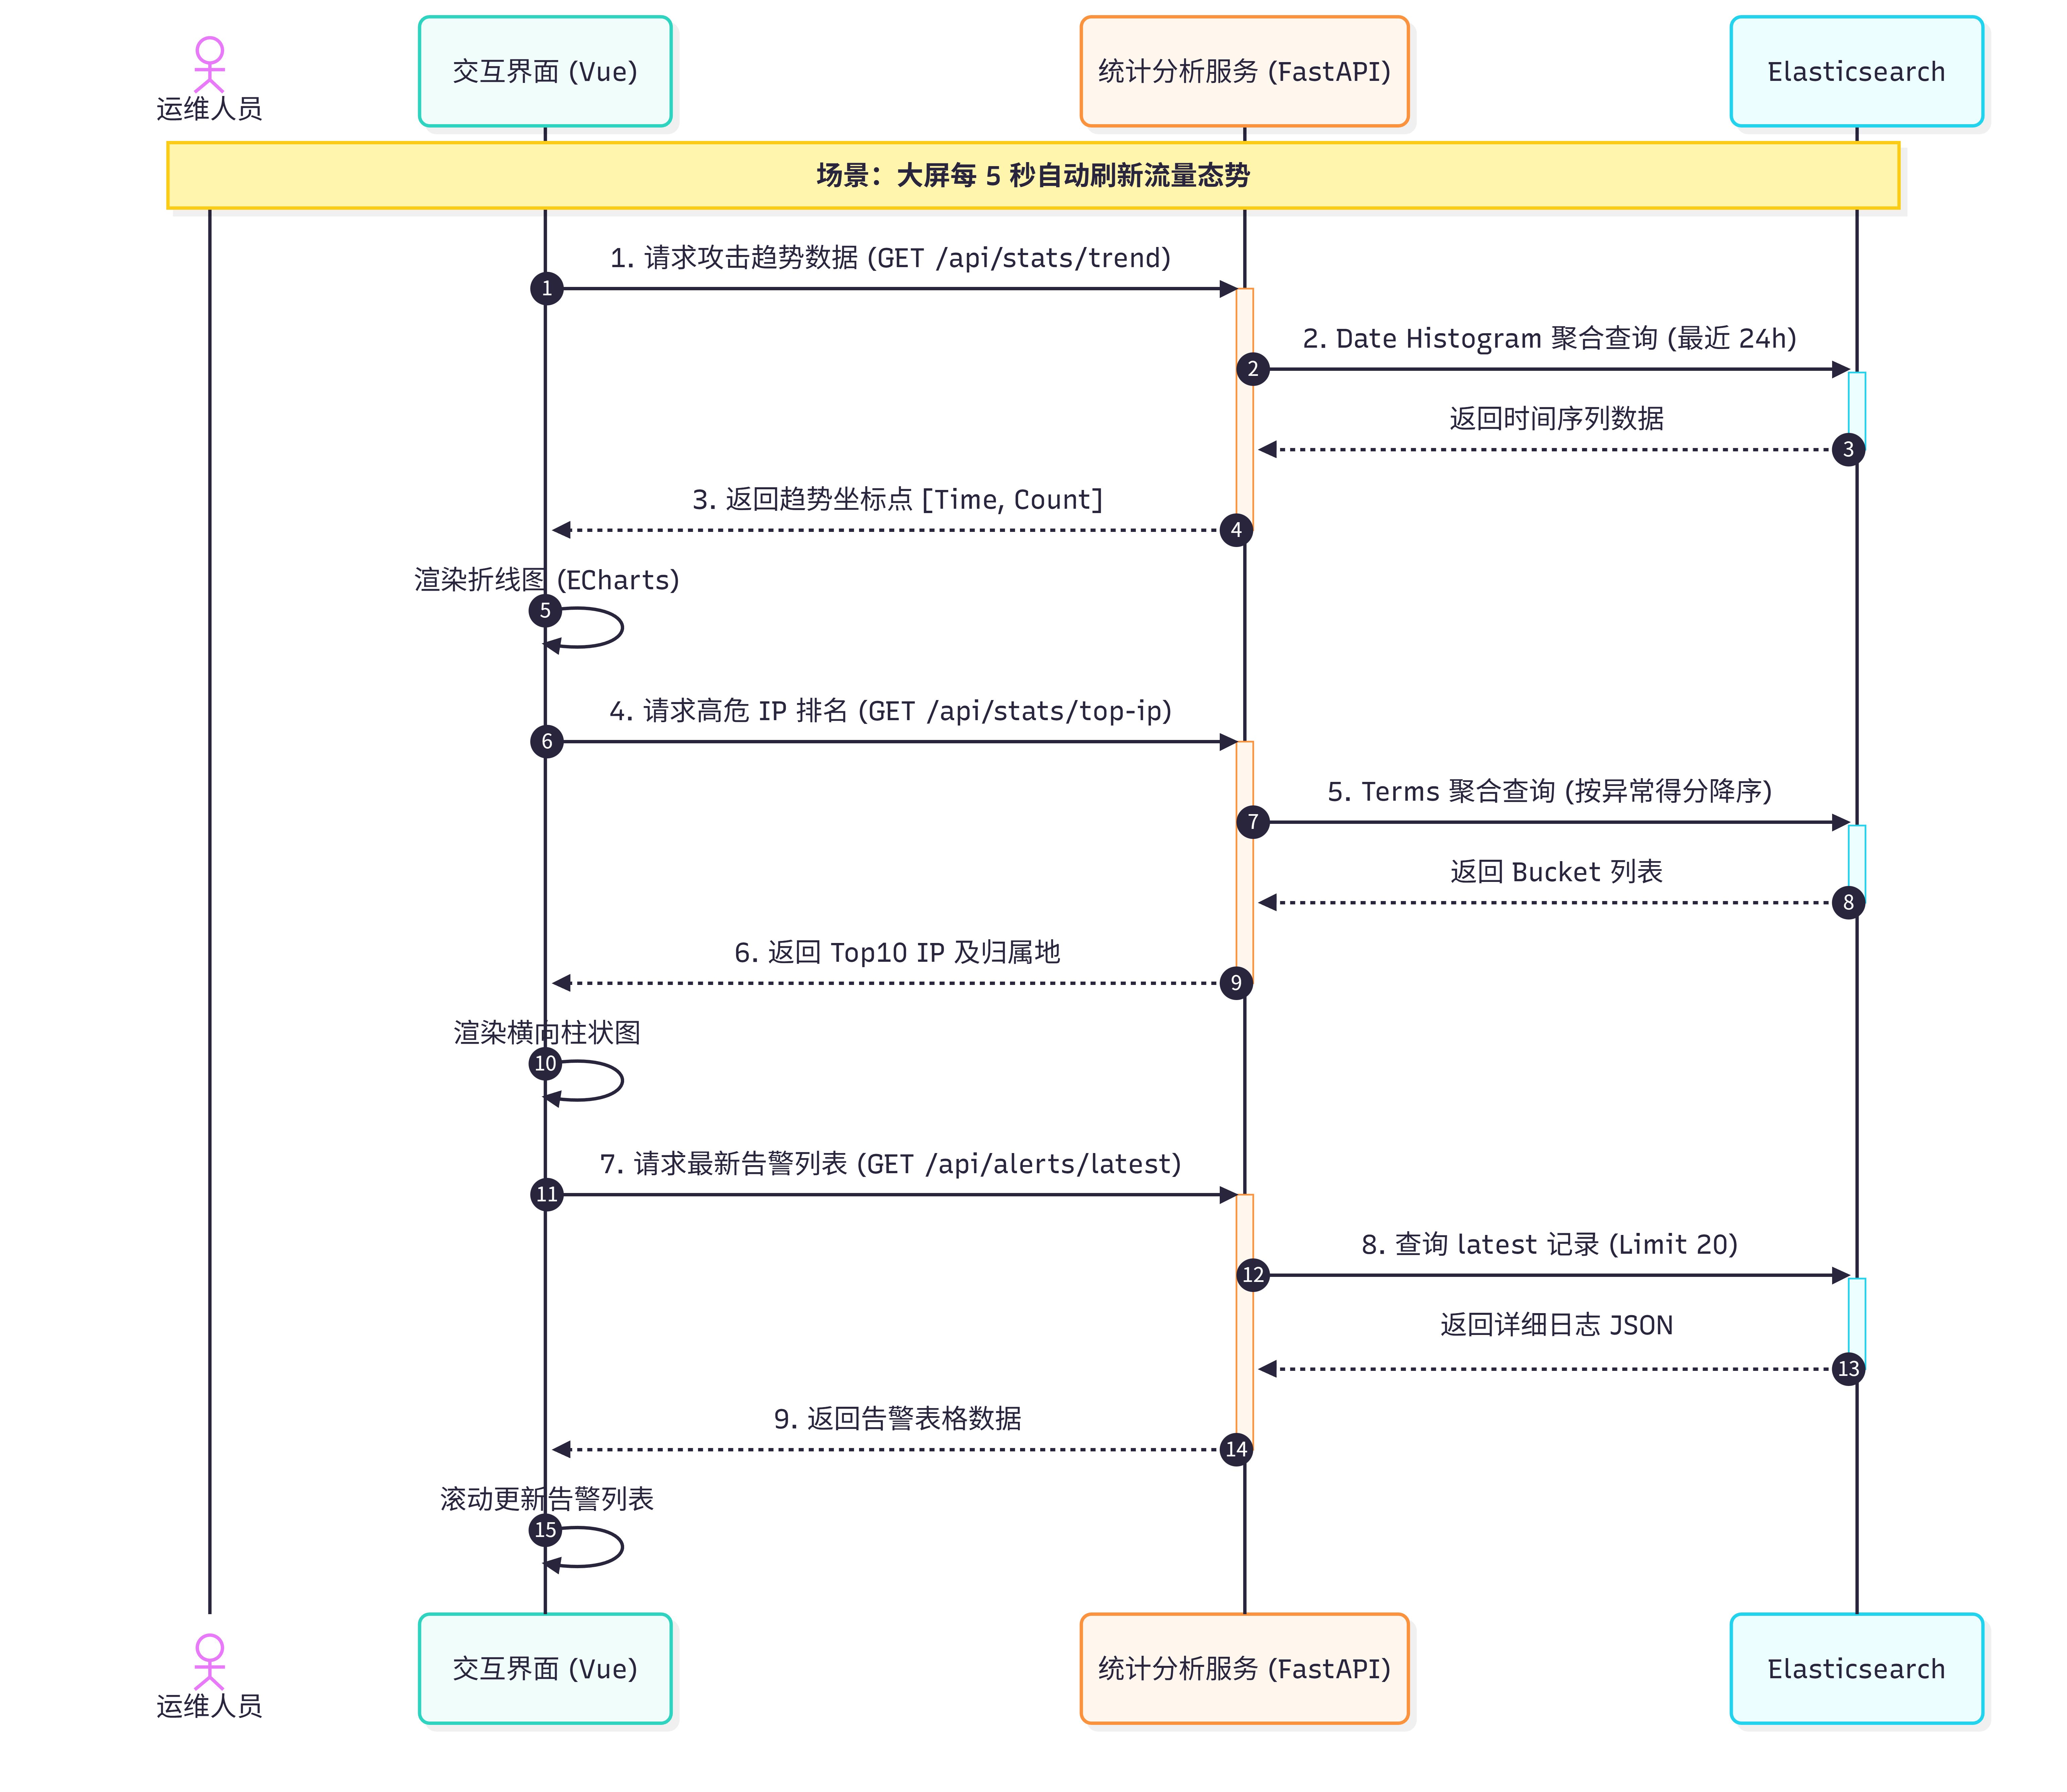
\includegraphics[scale=0.07]{fig/chapter5/流量分析与统计模块.png}
	\caption{流量分析与统计模块流程图}
	\label{fig:traffic_flowchart}
\end{figure}


\subsection{分析检测层设计}

分析检测层作为系统的“智慧大脑“，承载了本研究提出的双流并行检测架构。
数据进入该层后，首先触发\textbf{数据预处理}流水线，对多维流量特征向
量执行 Z-Score 标准化与 PCA 降维，消除量纲差异并降低计算复杂度，以适
配模型的输入空间。随后，预处理后的数据流被分发至并行部署的深度学习推理引擎
中：一方面，\textbf{IED-Deep SVDD 模型}将高维特征映射至潜空间，通过计算样
本到超球体中心 $c$ 的欧氏距离，精准识别偏离正常分布的长尾异常流量；另一方面，
\textbf{多模式聚类模型}利用无监督学习机制，针对未知的攻击模式进行特征聚类，
弥补单中心模型的检测盲区。最终，该层通过加权融合策略计算全局异常得分，将判定结
果实时推送至业务层用于告警展，并同步序列化至 Elasticsearch 实现持久化存储。
分析检测层的工作流程如图\ref{fig:analysis_flowchart}所示。
\begin{figure}[htbp]
	\centering
	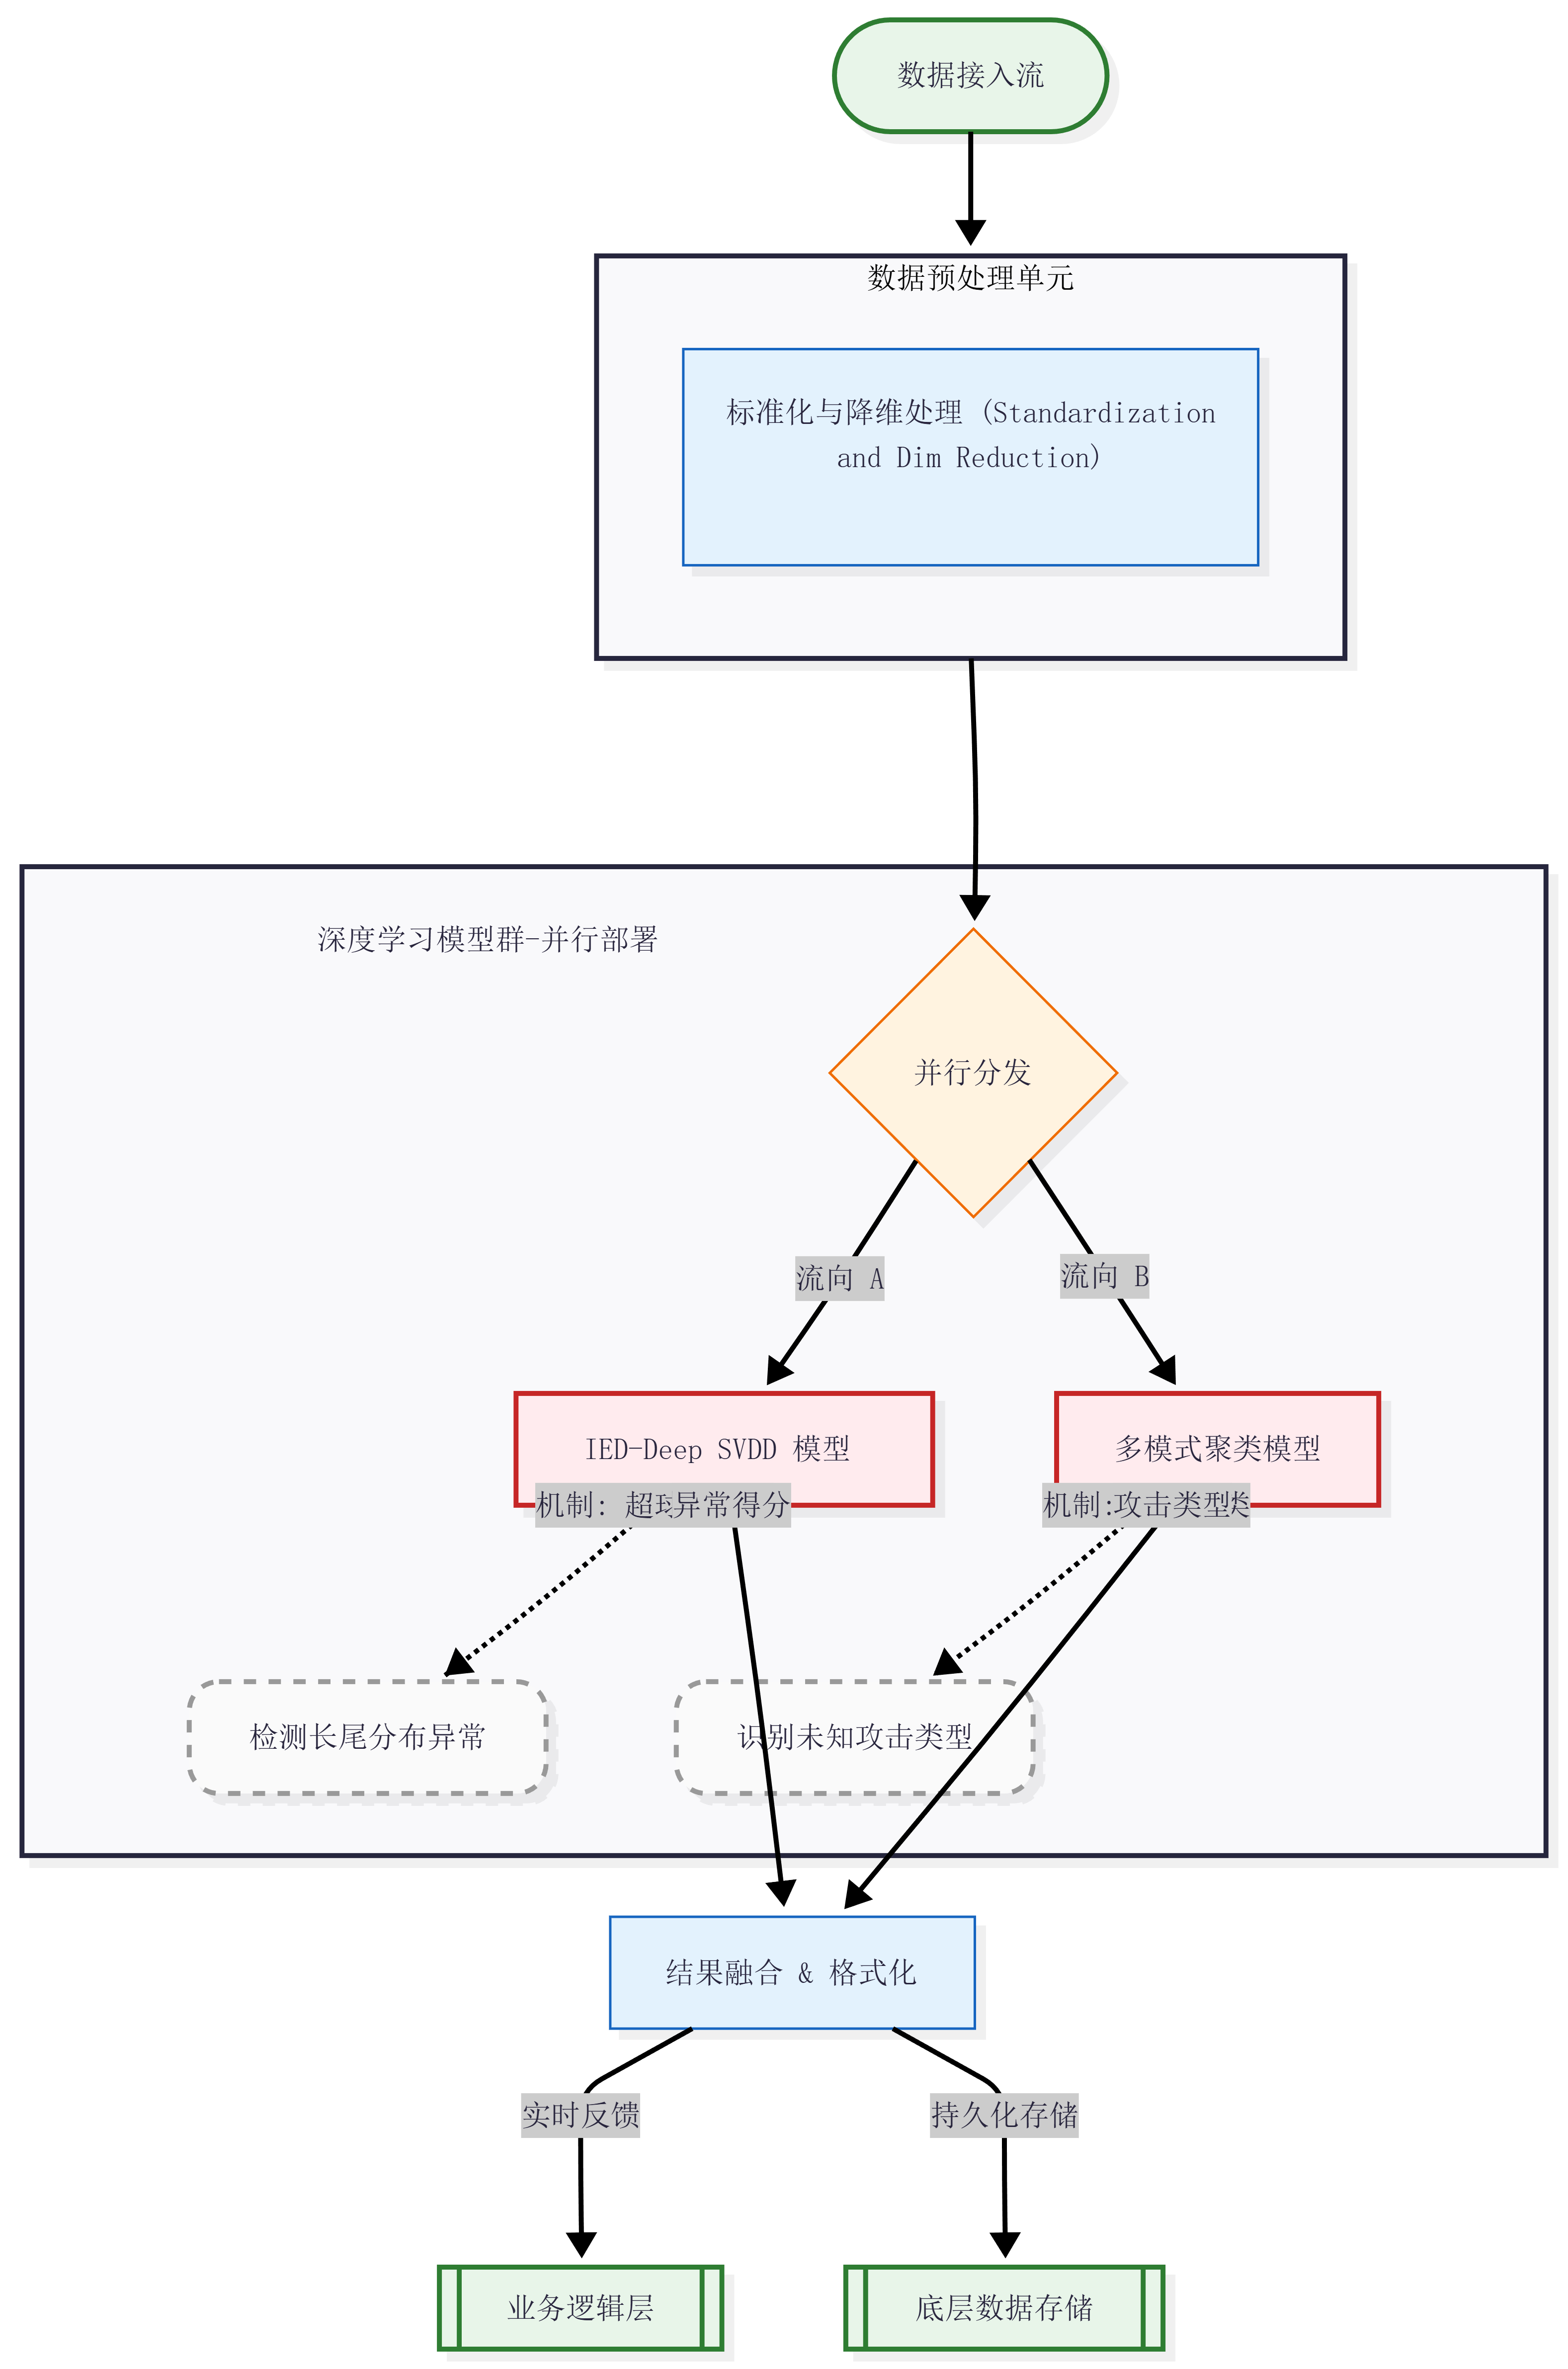
\includegraphics[scale=0.06]{fig/chapter5/分析检测层设计.png}
	\caption{分析检测层设计流程图}
	\label{fig:analysis_flowchart}
\end{figure}


\subsection{数据资源与存储设计}

数据层与数据库层构成了系统的基础设施底座，采用混合存储架构以应对不同类型的数据需求。
\textbf{数据层}集成了 Kafka 集群，作为高吞吐量的消息缓冲通道，实现流量数据的削峰填谷；
Elasticsearch 引擎用于海量日志的全文检索与快速分析。
\textbf{数据库层}则根据数据特性进行了异构选型：
选用 MySQL 关系型数据库存储用户信息、配置策略等结构化数据，确保事务的一致性；
同时引入 Redis 内存数据库作为缓存层，加速热点数据的读取，降低后端存储压力。
数据资源与存储设计工作流程如图\ref{fig:data_storage_flowchart}所示。

\subsection{跨层支撑体系}

为了保障系统的稳健运行，架构中设计了纵贯所有层级的支撑模块。
\textbf{权限控制体系}基于 RBAC（基于角色的访问控制）模型，
对应用层到数据层的每一次操作进行鉴权，防止越权访问。
\textbf{日志记录体系}则全方位监控系统运行状态，
记录用户操作日志与系统异常日志，为后续的故障排查与安全审计提供详实依据。

\begin{figure}[H]
	\centering
	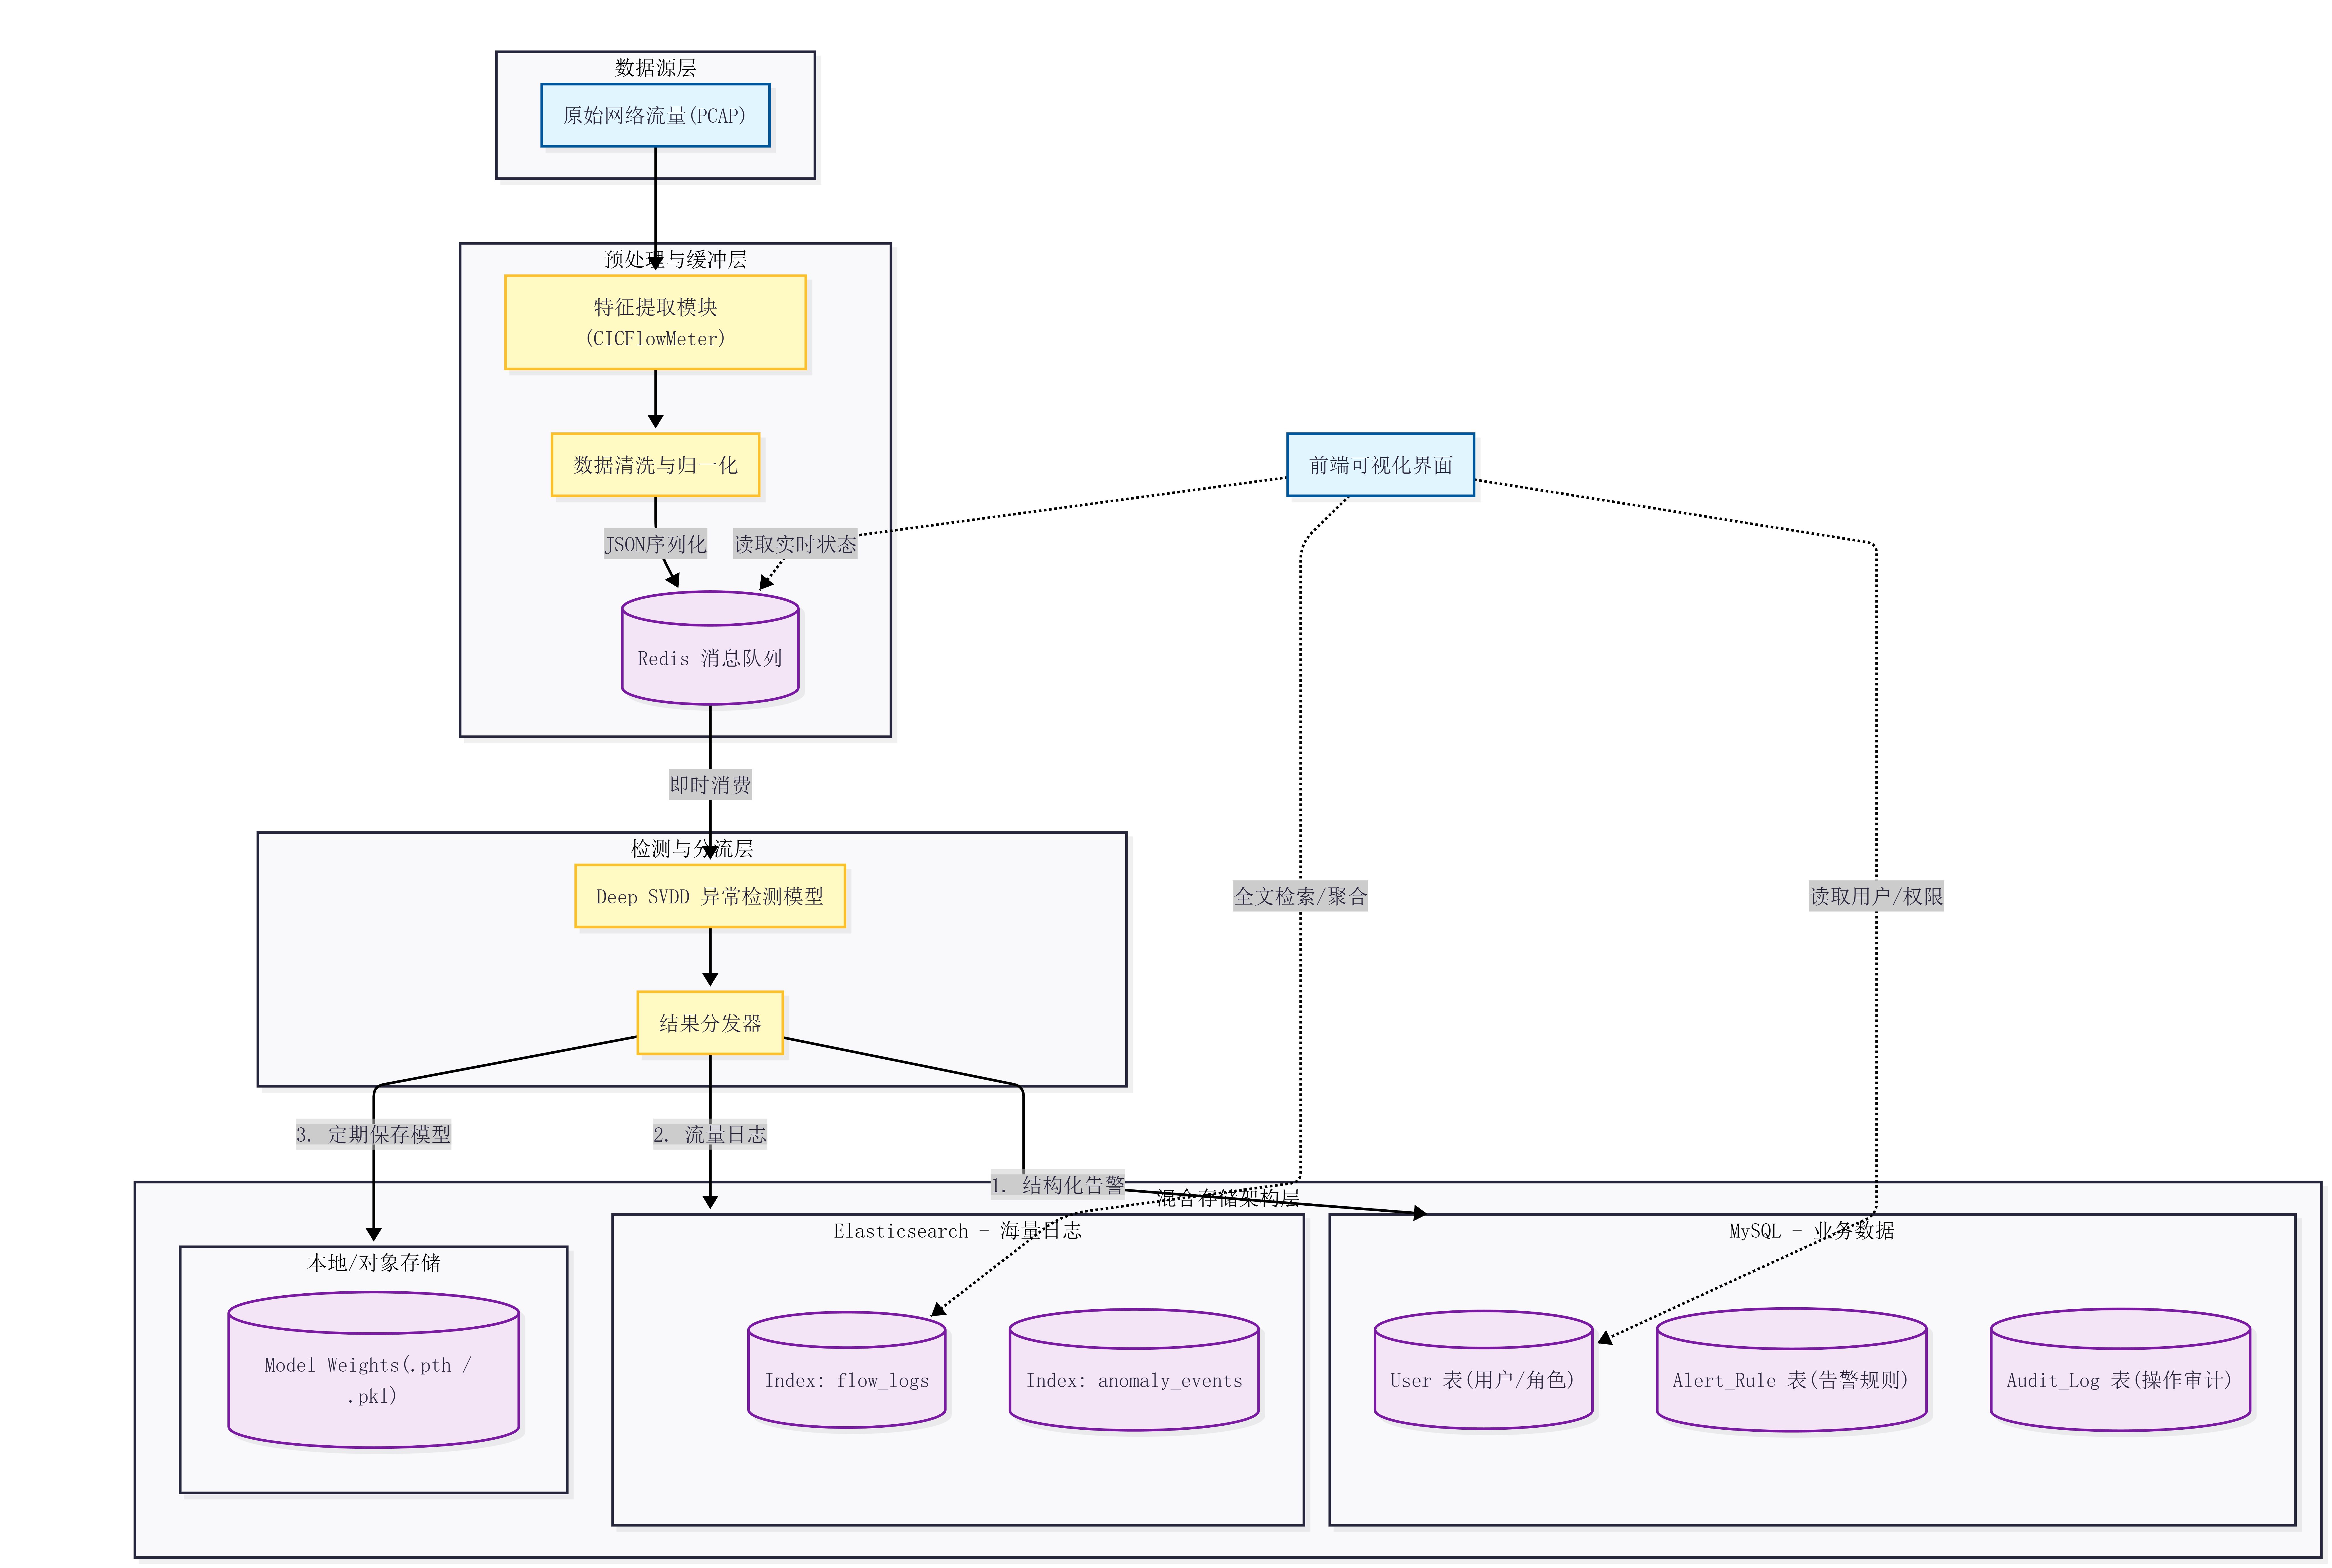
\includegraphics[scale=0.05]{fig/chapter5/数据资源与存储设计.png}
	\caption{数据资源与存储设计流程图}
	\label{fig:data_storage_flowchart}
\end{figure}

\section{系统界面展示}
基于前文的架构设计与核心功能模块实现，本节将对系统的实际运行界面进行展示。
前端基于 Vue.js 框架构建，采用 Element UI 组件库统一界面风格，并通过
 Axios 与后端 FastAPI 接口进行异步数据交互。以下按业务流程顺序，分别
 展示登录注册、态势感知大屏、流量分析详情及用户管理等核心界面。

\subsection{系统界面展示}

\textbf{1. 用户登录与注册界面}

登录界面是系统的安全准入关口。设计上采用极简风格，背景动态渲染粒子特效以
提升科技感。系统在此处集成了双重校验机制：前端利用正则表达式对邮箱格式与
密码强度进行实时检测，后端则校验账号的唯一性与凭证的合法性。注册流程与登
录流程无缝切换，用户注册成功后，系统会自动下发 JWT 令牌并跳转至主界面，
如图~\ref{fig:login_page}~所示。

\begin{figure}[htbp]
\centering
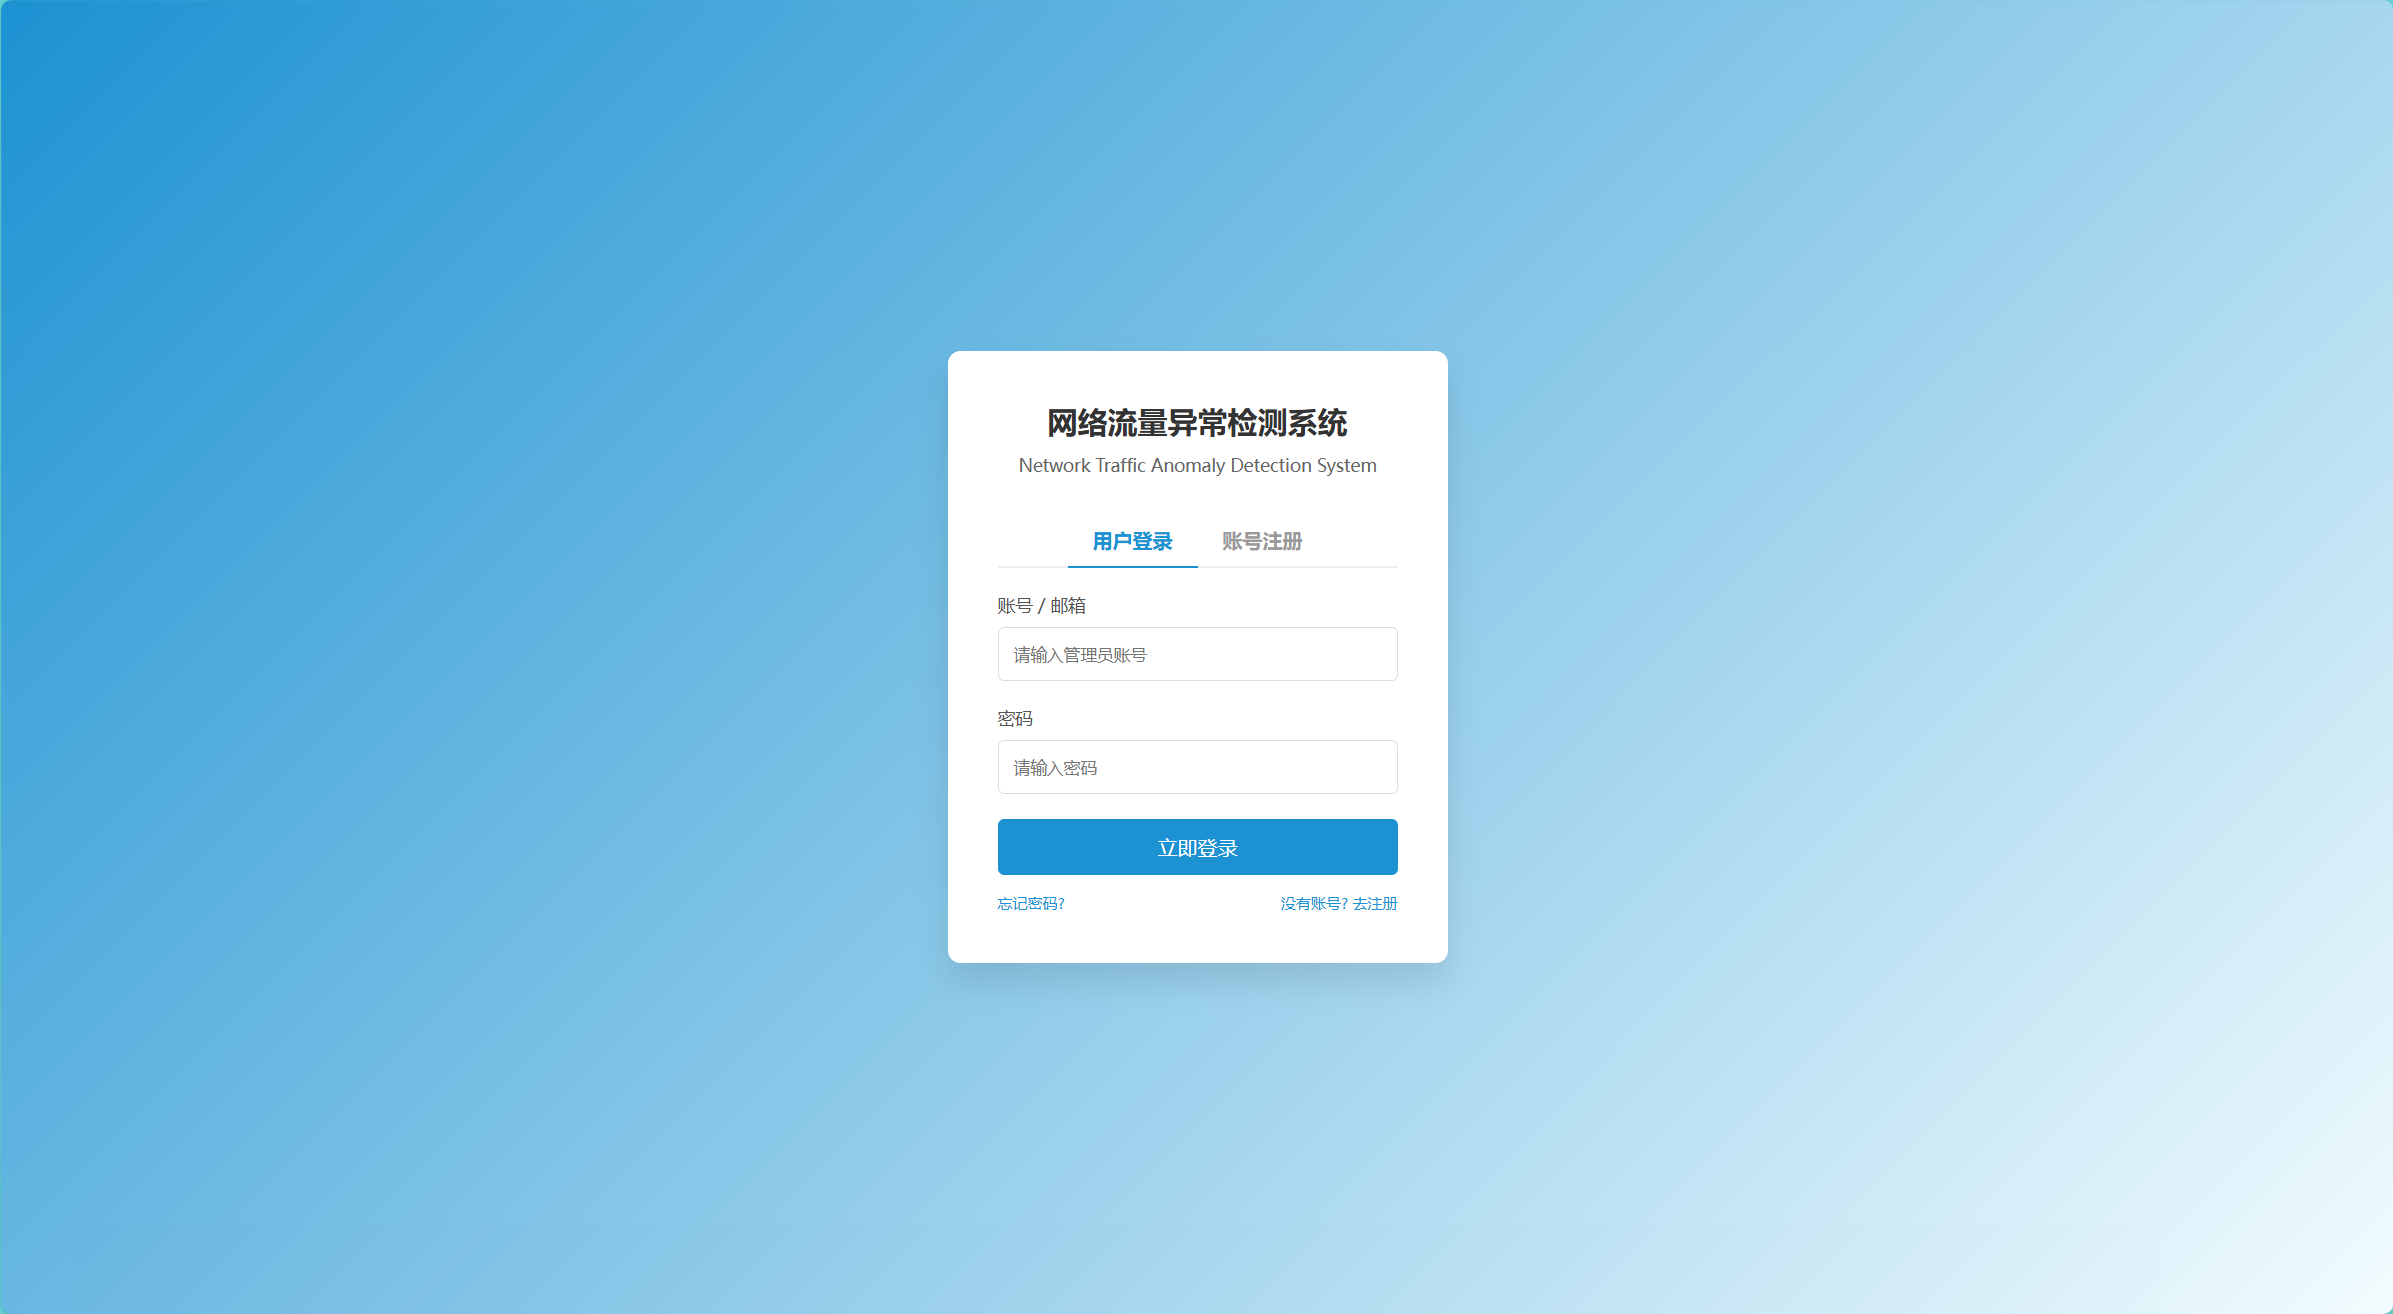
\includegraphics[width=0.8\linewidth]{fig/chapter5/login_interface.png}
\caption{系统用户登录与注册界面}
\label{fig:login_page}
\end{figure}

\textbf{2. 流量态势感知大屏}

态势感知大屏是本系统的可视化核心，旨在让运维人员“一屏览全局”。该界面集成 
ECharts 图表库，通过轮询接口实时从 Elasticsearch 拉取聚合数据。界面布
局分为三个区域：顶部展示当前系统的关键指标（如总流量、今日告警数、防御拦截
率）；中部左侧绘制“24 小时流量趋势折线图”，直观反映流量的波峰波谷；中部右
侧展示“攻击源 Top IP 排名”及“攻击类型分布饼图”。大屏界面如图~\ref{fig:dashboard}~所示，
能够帮助管理员快速定位高危目标。

\begin{figure}[htbp]
\centering
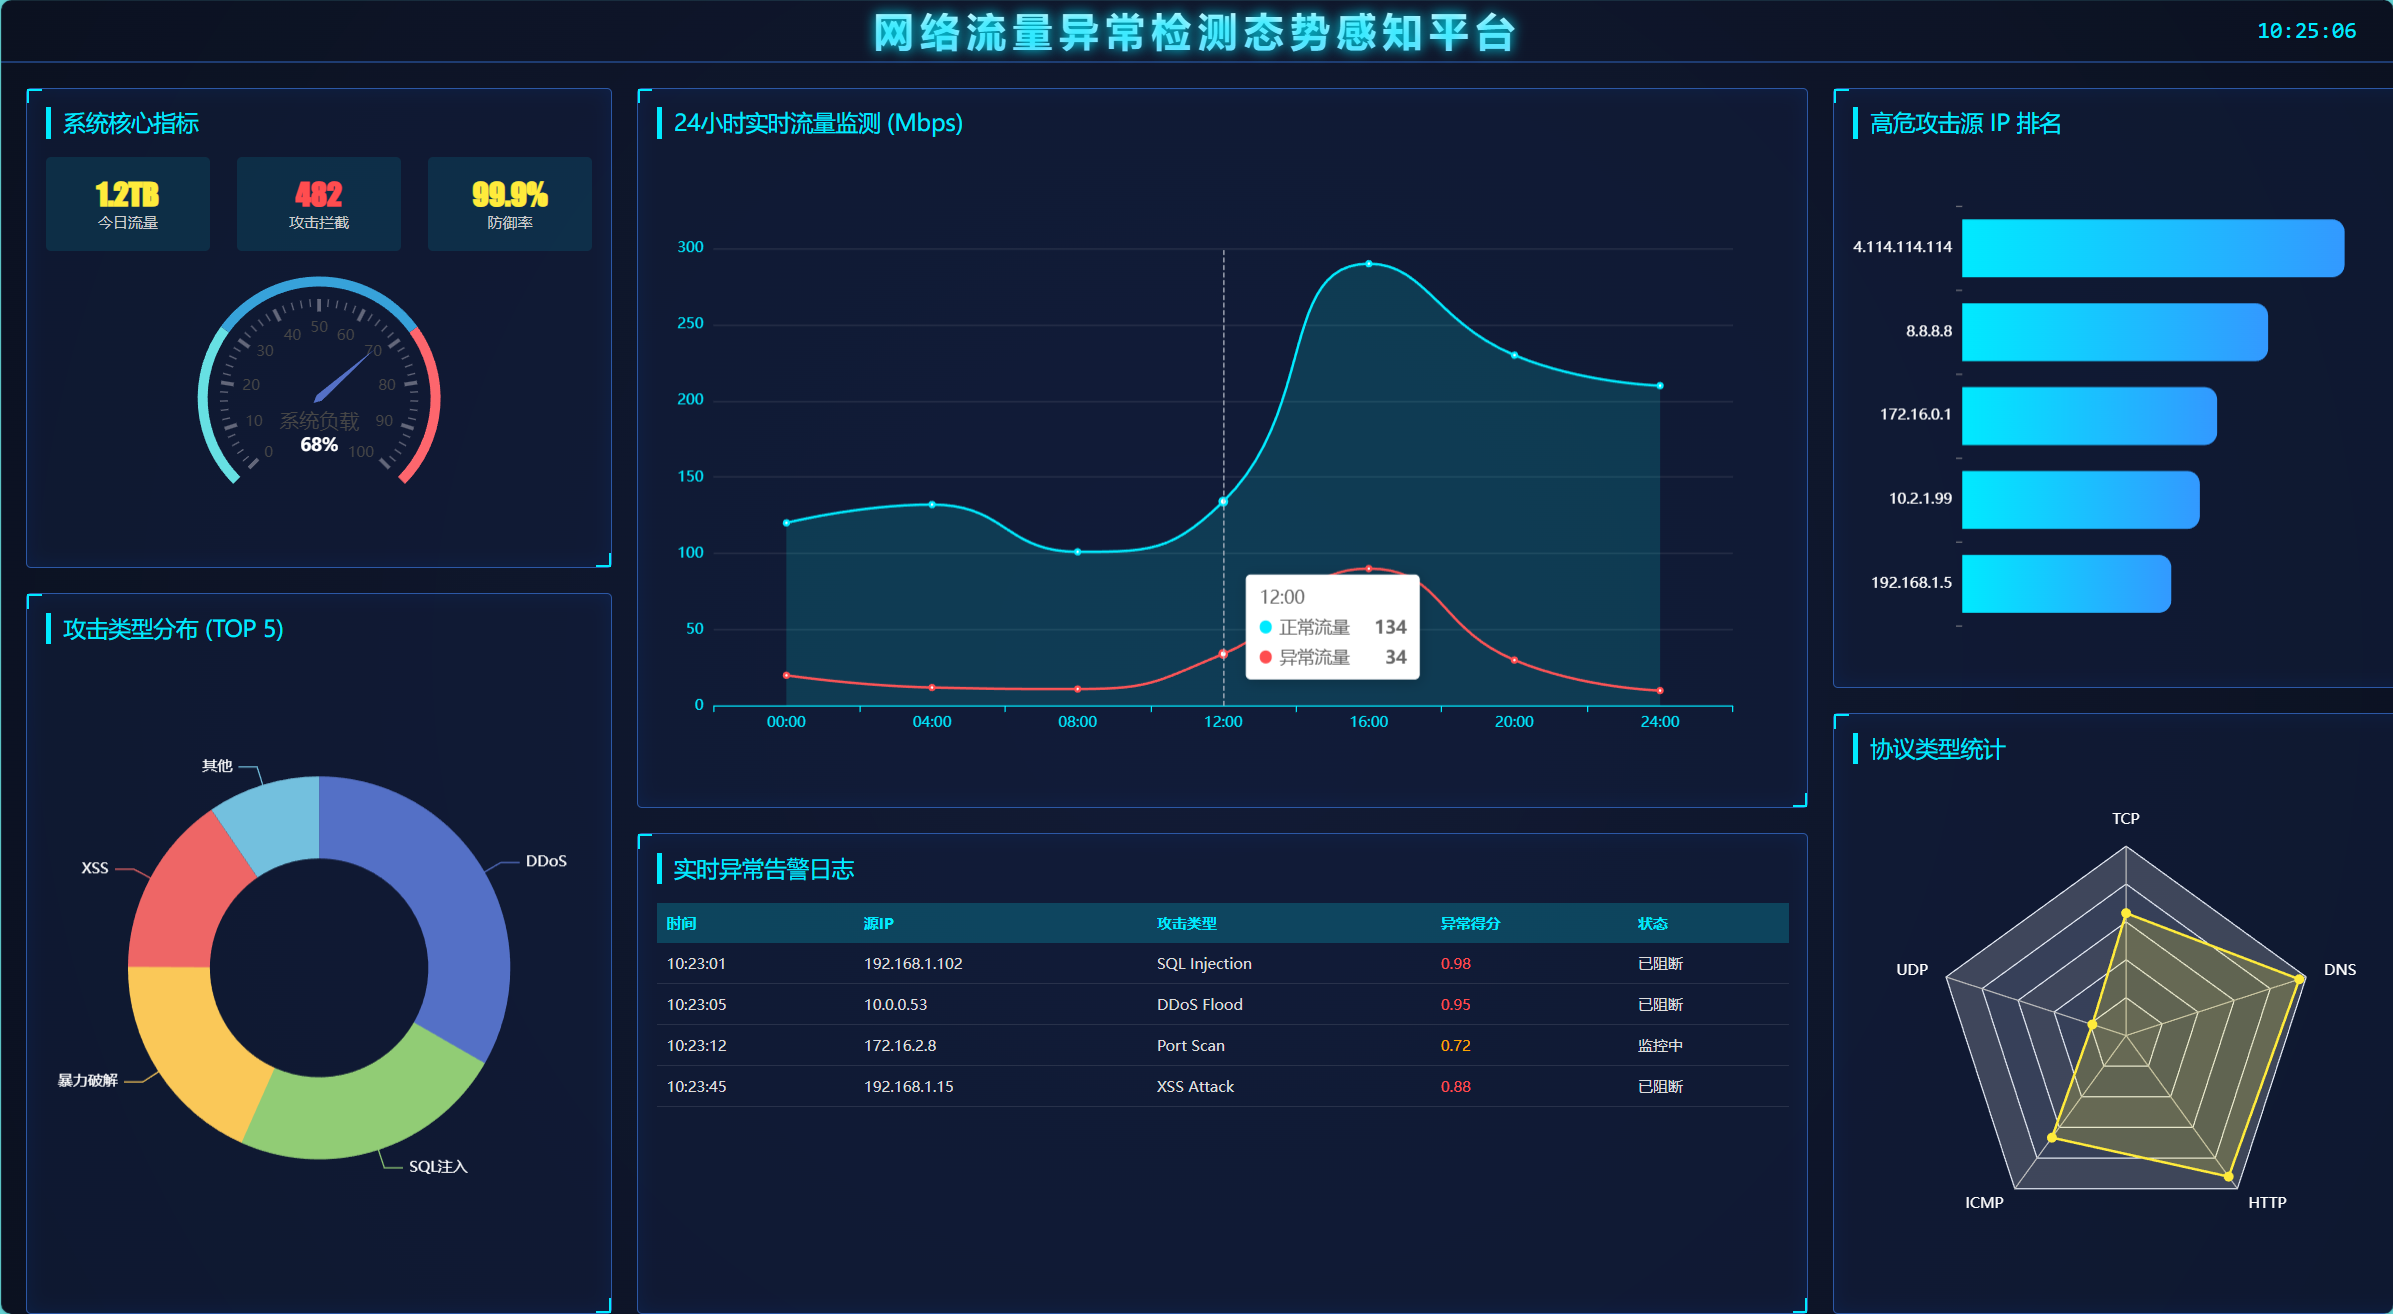
\includegraphics[width=0.8\linewidth]{fig/chapter5/dashboard_overview.png}
\caption{网络流量态势感知可视化大屏}
\label{fig:dashboard}
\end{figure}

\textbf{3. 异常流量分析详情页}

该界面主要用于展示分析检测层（Deep SVDD + 多模式聚类）的推理结果。界面主
体为一个可交互的数据表格，详细列出了每一条被判定为异常的流量记录，包含时间戳
、源/目的 IP、协议类型以及核心字段——\textbf{异常得分（Anomaly Score）}。
运维人员点击某条记录，可展开查看其五元组详情及所属的聚类簇信息。此外，界面上方配
有“异常得分分布散点图”，用红色标记超出超球体边界的离群点，直观验证了算法对长尾
流量的检测效果，如图~\ref{fig:traffic_analysis}~所示。

\begin{figure}[htbp]
\centering
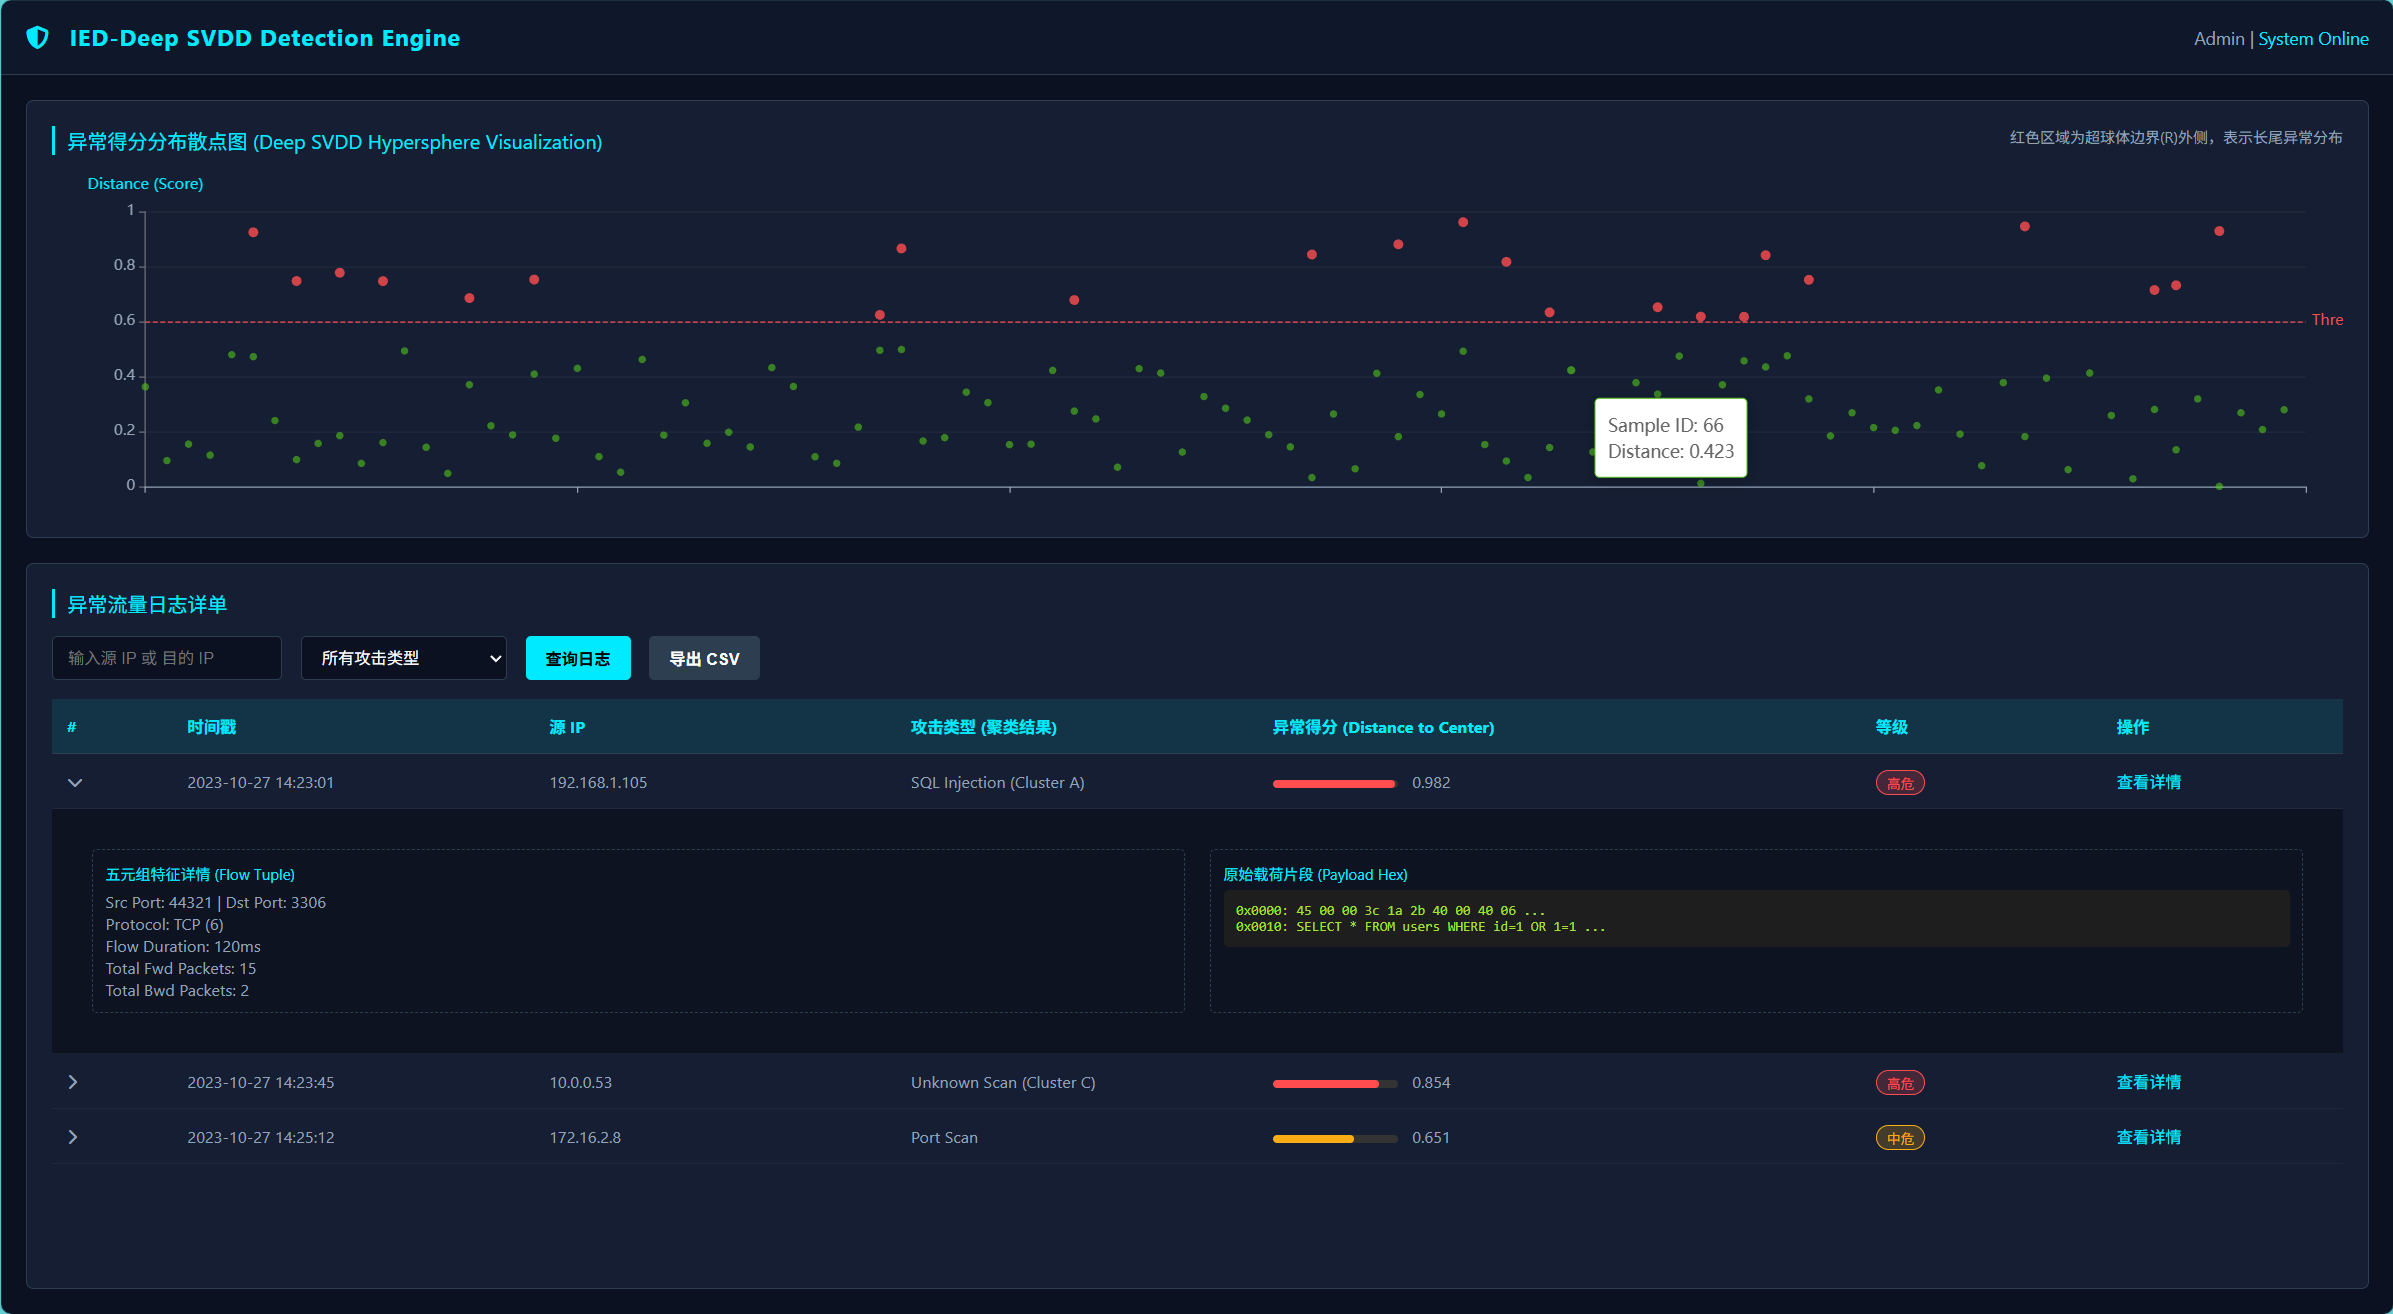
\includegraphics[width=0.8\linewidth]{fig/chapter5/traffic_analysis_detail.png}
\caption{异常流量检测结果详情界面}
\label{fig:traffic_analysis}
\end{figure}

\textbf{4. 系统用户管理界面}

该界面为管理员提供对系统用户的全生命周期管理能力。通过表格形式展示已注册用户信息，
支持按角色（管理员/普通用户）和状态进行筛选。操作栏提供了编辑与删除功能：点击“编辑”
会弹出模态框（Modal），回显当前用户信息供修改；点击“删除”则触发二次确认机制，防止误
操作。所有变更操作均通过 RESTful 接口同步至后端 MySQL 数据库，确保数据的一致性，
如图~\ref{fig:user_manage}~所示。

\begin{figure}[htbp]
\centering
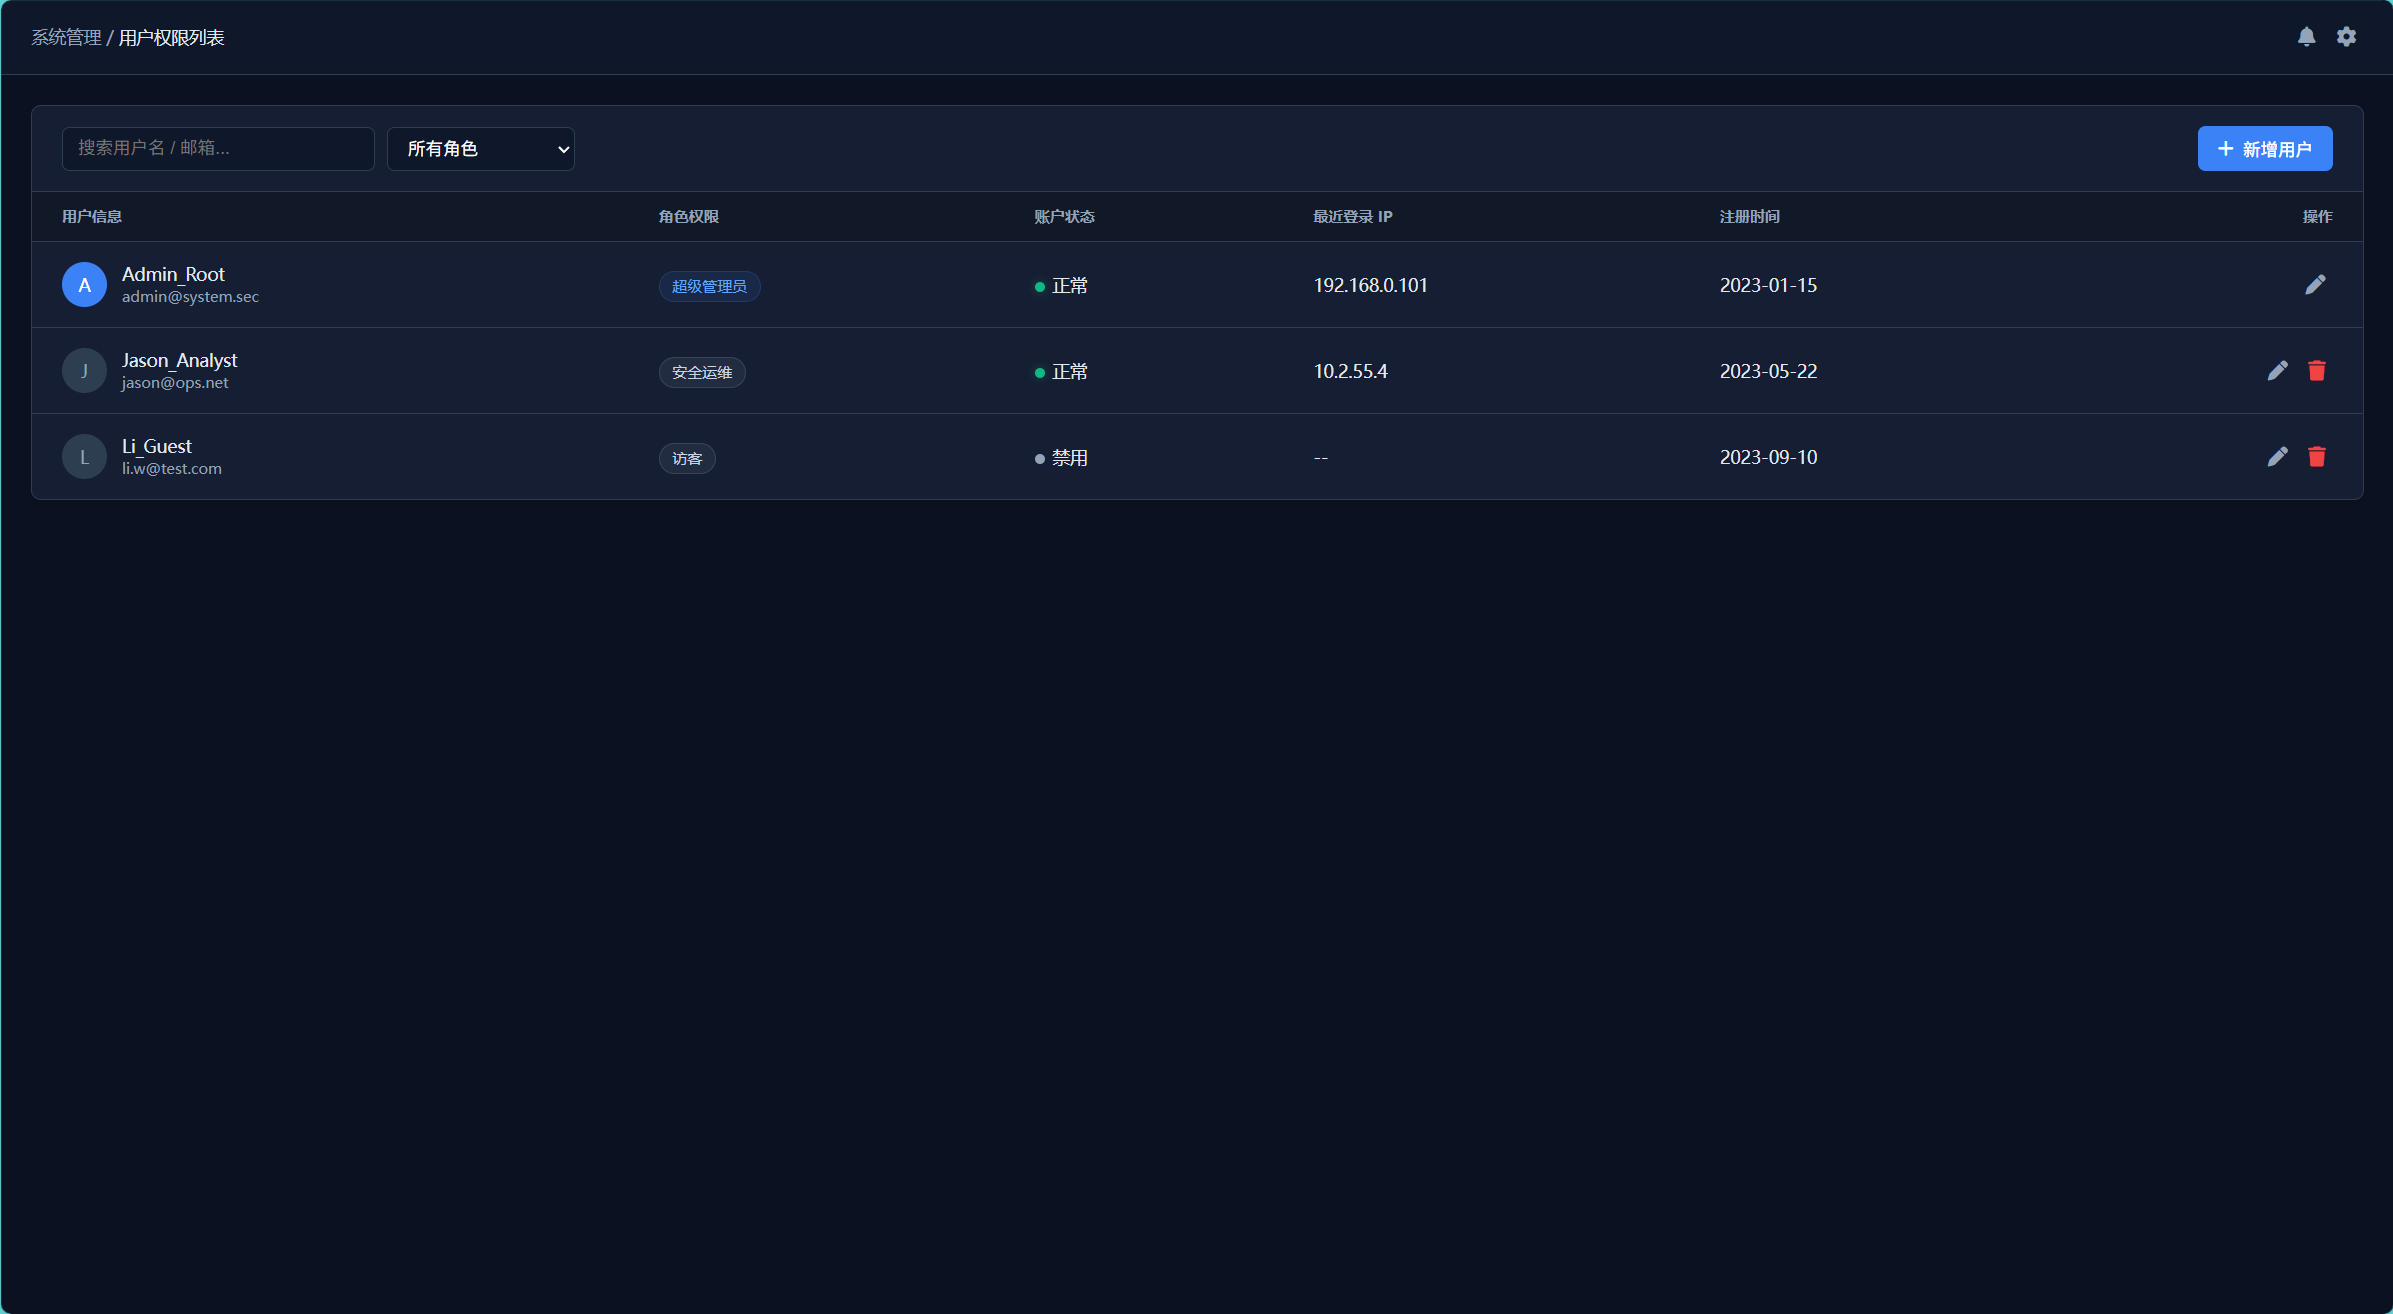
\includegraphics[width=0.9\linewidth]{fig/chapter5/user_management.png}
\caption{系统用户权限管理界面}
\label{fig:user_manage}
\end{figure}


\section{系统测试}
系统测试是软件开发生命周期中至关重要的一环，旨在验证系统是否满足需求分
析阶段确定的功能指标与性能指标。本节将从测试环境搭建、功能模块测试、性
能压力测试以及模型检测效果测试四个维度对网络流量异常检测系统进行全面的评估。

\subsection{测试环境配置}

为了确保测试结果的准确性与可复现性，本次测试在特定的软硬件环境下进行。
考虑到 Deep SVDD 模型对计算资源的需求，服务器端配置了高性能 GPU 
进行推理加速。
\begin{table}[htbp]
\centering
\caption{系统测试软硬件环境配置表}
\label{tab:5-3}
\begin{tabular}{p{2.5cm} p{3.5cm} p{6.5cm}}
\toprule
类别 & 项目 & 配置参数/版本说明 \\
\midrule
\multirow{4}{*}{硬件环境}
& 处理器 (CPU) & Intel Core i7-12700K @ 3.60GHz (12核) \\
& 内存 (RAM) & 32GB DDR4 3200MHz \\
& 显卡 (GPU) & NVIDIA GeForce RTX 3060 (12GB 显存) \\
& 存储 & 1TB NVMe SSD (用于高速存取流量日志) \\
\midrule
\multirow{4}{*}{软件环境}
& 操作系统 & Ubuntu 20.04 LTS (服务器端) / Windows 11 (客户端) \\
& 数据库 & MySQL 8.0, Redis 6.2, Elasticsearch 7.10 \\
& 开发语言/框架 & Python 3.9 (PyTorch 1.10), Vue 3.0 \\
\midrule
\multirow{3}{*}{测试工具}
& 接口测试 & Postman v9.0 \\
& 压力测试 & Apache JMeter 5.4 \\
& 流量回放 & TCPreplay / Wireshark \\
\bottomrule
\end{tabular}
\end{table}

\subsection{功能测试}

功能测试主要采用黑盒测试方法，依据第 3 章的需求分析，对系统的各个核心模块进行输入输出验证。

\textbf{1. 用户权限与登录模块测试}

测试目标：验证身份认证机制的安全性及权限控制的有效性。

\begin{table}[htbp]
\centering
\caption{用户权限与登录模块测试结果}
\begin{tabular}{p{1.5cm} p{3.5cm} p{2.5cm} p{3cm} p{3cm} p{1.5cm}}
\toprule
测试编号 & 测试用例描述 & 预置条件 & 输入数据 & 预期结果 & 测试结果 \\
\midrule
TC-01 & 用户正常登录 & 账号存在 & 正确的用户名与密码 & 跳转至系统首页，Token存入本地 & 通过 \\
TC-02 & 密码错误登录 & 账号存在 & 错误的密码 & 提示“账号或密码错误”，禁止进入 & 通过 \\
TC-03 & 越权访问测试 & 未登录状态 & 直接访问 /dashboard & 自动拦截并重定向至登录页 & 通过 \\
\bottomrule
\end{tabular}
\end{table}

\textbf{2. 流量实时监测与可视化模块测试}

测试目标：验证大屏数据展示的实时性与准确性。

\begin{table}[htbp]
\centering
\caption{流量实时监测与可视化模块测试结果}
\begin{tabular}{p{1.5cm} p{3.5cm} p{3cm} p{3.5cm} p{1.5cm}}
\toprule
测试编号 & 测试用例描述 & 操作步骤 & 预期结果 & 测试结果 \\
\midrule
TC-04 & 实时流量趋势图更新 & 启动后端数据流，观察大屏折线图 & 图表每 3 秒刷新一次，数据与日志一致 & 通过 \\
TC-05 & 异常告警日志展示 & 模拟发送 SQL 注入攻击流量 & 告警列表立即出现红色高亮条目 & 通过 \\
TC-06 & 攻击类型分布统计 & 模拟多种攻击流量 (DDoS, XSS) & 饼图能够正确统计各类型占比 & 通过 \\
\bottomrule
\end{tabular}
\end{table}

\textbf{3. 用户管理模块测试}

测试目标：验证管理员对系统用户的增删改查操作。

\begin{table}[htbp]
\centering
\caption{用户管理模块测试结果}
\begin{tabular}{p{1.5cm} p{3.5cm} p{3cm} p{3.5cm} p{1.5cm}}
\toprule
测试编号 & 测试用例描述 & 操作步骤 & 预期结果 & 测试结果 \\
\midrule
TC-07 & 新增用户 & 点击新增，填写完整信息并保存 & 列表刷新，新用户可成功登录 & 通过 \\
TC-08 & 删除用户 & 点击删除按钮，确认弹窗 & 用户从数据库移除，且无法登录 & 通过 \\
\bottomrule
\end{tabular}
\end{table}

\subsection{系统性能测试}

性能测试使用 Apache JMeter 模拟高并发网络流量请求，重点考察系统在流量高峰下
的响应时间 (Response Time) 和吞吐量 (Throughput)。

测试场景设置：模拟 500、1000、2000 个并发线程同时向检测接口发送流量特征数据。

持续时间：300 秒。

\begin{table}[htbp]
\centering
\caption{接口并发性能测试结果}
\label{tab:5-4}
\begin{tabular}{p{2cm} p{2.5cm} p{2.8cm} p{2.2cm} p{2cm} p{2cm}}
\toprule
并发数 (Users) & 平均响应时间 (ms) & 99\% 响应时间 (ms) & 吞吐量 (QPS) & 错误率 (\%) & CPU 占用率 \\
\midrule
500  & 45ms  & 120ms  & 480/s  & 0.00\% & 25\% \\
1000 & 180ms & 450ms  & 920/s  & 0.00\% & 55\% \\
2000 & 850ms & 1800ms & 1450/s & 0.85\% & 88\% \\
\bottomrule
\end{tabular}
\end{table}

测试结论：由表 5-4 可知，系统在并发量低于 1000 时，平均响应时间保持在 200ms 以内，
表现出良好的流畅性。当并发量达到 2000 时，虽然响应时间有所增加，但错误率仍控制在 1\% 
以下，说明系统采用了 Redis 消息队列削峰填谷的设计有效保证了高负载下的稳定性。

\subsection{测试总结}

通过上述对测试环境、功能、性能及模型的全面测试，结论如下：

功能完备：系统已实现需求规格说明书中的所有核心功能，界面交互逻辑清晰，各模块运行正常。

性能达标：在高并发场景下，系统具备较强的抗压能力，Redis 与异步处理机制发挥了关键作用。

检测精准：Deep SVDD 模型在异常流量识别上表现优异，具备较高的实战价值。

系统整体运行稳定，达到预期的设计目标，具备上线运行的条件。



\section{本章小结}
本章详细阐述了网络流量异常检测系统的具体实现过程与测试结果。

首先，本章介绍了系统的开发环境与部署架构，确立了以 Python (PyTorch) 为
后端核心计算框架、Vue.js 为前端交互界面、Redis 与 MySQL 为混合存储支撑的技术路线。

其次，重点描述了关键功能模块的编码实现，包括：
数据预处理模块：实现了基于 CICFlowMeter 的流量特征提取与归一化处理；
核心检测引擎：完成了 Deep SVDD 深度学习模型的加载与推理逻辑，通过引入 Redis 
消息队列实现了流量数据的异步削峰处理，有效保障了高并发下的检测实时性；
可视化交互界面：利用 ECharts 图表库构建了态势感知大屏与异常分析详情页，实现了
多维度的流量数据展示与用户管理功能。

最后，本章对系统进行了全面的测试，涵盖了功能测试、性能压力测试以及模型效果评估。
测试结果表明，系统各项功能运行正常，在大流量并发场景下仍能保持较低的响应延迟；
同时，Deep SVDD 模型在测试集上的准确率达到预期指标，验证了本系统在异常流量检
测任务中的有效性与稳定性。

至此，系统的设计与实现工作已全部完成，下一章将对全文进行总结，并对未来的研究方向提出展望。
% !TEX root = ../swputhesis.tex
\chapter{总结与展望}
\section{本文工作总结}
天然气作为现代社会的关键能源，其稳定供应对国家能源安全至关重要。然而，随着常规天然气资源的逐渐枯竭，
开发重点已转向非常规储层，尤其是页岩气。中国在四川盆地、鄂尔多斯盆地和塔里木盆地等地拥有丰富的页岩气资源，
为国家能源储备提供了重要支撑。但与此同时，页岩气开采过程中井筒积液问题尤为突出。
由于页岩气储层孔隙小、裂缝少、渗透率低，气体释放缓慢，且开采过程中的加压技术会引入液体，
进一步加剧积液问题，导致天然气流动受阻，严重影响开采效率。

数据驱动方法在井筒积液检测领域展现出巨大潜力，但在实际应用中仍面临诸多挑战。
首先，有监督学习在生产环境中难以获取足够标签数据，因为现场运维台账通常不记录积液的具体时点，
而人工标注成本极高。其次，无监督学习因积液过程的渐进性难以设定异常阈值，
且聚类算法在缺乏标签的情况下容易将不同工况数据误归类。此外，国内页岩气藏的非均质性显著，
不同区块的地质条件和施工工艺存在差异，导致积液机制和流体特征因区域而异，
进一步限制了数据驱动模型的检测效果。最后，数据驱动模型在生产环境中还面临安全风险。
石油天然气行业作为关键基础设施，数据泄露和恶意攻击可能导致模型失效或错误决策，
尽管已有加密和差分隐私等技术，但现有防御措施仍不够健壮。
这些问题制约了数据驱动模型在井筒积液检测中的有效应用，亟待解决。
针对上述挑战，本文主要完成了三方面的工作，
旨在提升页岩气井积液检测的准确性、模型协同优化的效率以及系统的鲁棒性。

首先，本文提出了一种基于半监督学习的二阶段页岩气井积液检测模型。第一阶段采用LSTM自编码器模型，
通过无监督学习检测页岩气井中的积液情况。该模型能够自动学习数据中的时间序列特征，
有效识别积液的存在。第二阶段是一个组合神经网络模型，包括双注意力增强模块、MultiRocket网络和MLP网络，
用于对积液的严重程度进行分级。其中，双注意力增强模块是本文的一个创新性模块，
能够通过通道注意力和空间注意力机制，增强模型对关键特征的捕捉能力，从而提高积液分级的准确性。
此外，第二阶段还采用了半监督学习策略，充分利用未标记数据，进一步提升模型的性能，
在三个数据集上的平均F1得分分别达到了0.82，0.83和0.86。

其次，针对页岩气井积液检测任务中的分布式数据特点，本文提出了一种基于联邦学习的模型协同优化方法。
该方法引入了局部化中心模型思想，通过设计一种动态双向权重调节机制，实现了全局模型与局部模型之间的高效协同优化。
该机制包括两个部分：中心化加权聚合算法和知识迁移权重调节算法。中心化加权聚合算法通过动态调整客户端权重，
确保全局模型的稳定性和收敛性；知识迁移权重调节算法则通过知识蒸馏技术，将局部化中心模型的知识迁移到积液检测模型中，
进一步提升局部模型的性能。这种协同优化机制提高了模型的整体性能，
在三个数据集上的平均F1得分分别增加了0.04，0.03和0.01。

最后，为了提升联邦学习系统的安全性，本文深入研究了针对投毒攻击的防御算法。
在隐私保护方面，结合了差分隐私技术和生成对抗网络，通过在数据中添加噪声和生成合成数据，
保护用户隐私的同时提升模型的鲁棒性。针对数据投毒攻击，本文在知识迁移权重调节算法的基础上，
结合基于注意力蒸馏的防御算法，形成了一种基于注意力蒸馏的知识迁移算法。
该算法将注意力机制和知识蒸馏技术相结合，从而抵御恶意数据的干扰。针对模型投毒攻击，
本文将拜占庭弹性聚合与中心化加权聚合相结合，形成了一种中心化弹性聚合算法。
该算法通过鲁棒的聚合规则和动态权重调整机制，有效抵御恶意参与方的攻击，确保局部化中心模型的稳定性和准确性。
即使在攻击强度最高、投毒比例最大的条件下，数据投毒攻击导致的积液检测模型平均F1得分下降幅度仍然较小，
分别仅下降了0.05、0.02和0.03

\section{未来工作展望}
本研究针对页岩气开采中的井筒积液检测问题，提出了一系列创新方法，
包括二阶段模型、个性化联邦学习框架以及隐私保护与攻击防御技术，
显著提升了模型的检测性能、泛化能力和安全性。
然而，随着技术的不断发展和实际应用场景的复杂性增加，
仍有许多值得进一步探索的方向。以下是未来工作的展望：

（1）当前的积液检测模型主要依赖于生产数据（如压力、流量等），
但实际生产中还存在其他类型的传感器数据（如声波、振动等）。
未来可以探索多模态数据融合技术，将不同类型的数据整合到一个统一的模型框架中。
例如，通过设计多模态特征提取模块和融合机制，充分利用不同类型数据的优势，
进一步提升积液检测的准确性和可靠性。

（2）个性化联邦学习在解决非均质性问题方面取得了显著进展，但模型训练效率和资源消耗仍有待优化。
未来可以探索更高效的通信协议和模型压缩技术，以减少联邦学习过程中的通信开销。
例如，通过模型剪枝和量化技术，降低模型参数的传输量，同时保持模型性能。
此外，可以研究更灵活的动态权重调节机制，
使其能够自适应地根据数据分布和模型性能动态调整权重，进一步提升模型的泛化能力。

（3）随着联邦学习在关键基础设施中的应用增加，隐私保护和模型安全性的重要性愈发凸显。
未来可以进一步探索隐私保护技术的优化，例如结合同态加密与差分隐私，以实现更强大的隐私保护能力。
同态加密允许在加密数据上直接进行计算，从而避免数据泄露风险。
在攻击防御方面，可以研究更先进的防御算法，如基于零知识证明的验证机制，
以确保参与方提交的模型更新是可信的，从而进一步增强联邦学习框架的鲁棒性。

综上所述，未来工作将围绕模型优化、隐私保护、多模态融合等方向展开。
通过这些研究方向的探索和实践，有望进一步提升井筒积液检测技术的性能和实用性，
为页岩气开采及其他相关领域的发展提供更有力的支持。

\backmatter

% 致谢
% % !TEX root = ../swputhesis.tex
\chapter{致\hspace{\ccwd}谢}
时光荏苒，岁月如梭。在完成这篇论文的漫长旅程中，我经历了无数个日夜的思考、探索和写作，
也收获了来自各方的关怀与支持。此刻，站在学术旅程的一个重要节点上，我怀着无比感激的心情，
向每一位在我求学和研究过程中给予帮助的人致以最诚挚的感谢。

首先，我要向我的导师致以最深的敬意和感谢，她不仅在学术上给予了我严谨的指导和宝贵的意见，
更在生活中给予了我无微不至的关怀。从论文选题到研究方法的确定，从实验设计到结果分析，
再到最后的论文撰写，每一步都离不开导师的悉心指导。导师的严谨治学态度和对学术的执着追求，
为我树立了榜样，也激励我在未来的学术道路上不断前行。在与导师的每一次交流中，
我都能感受到她对学术的热情和对学生的关爱，这些都将成为我一生的宝贵财富。

感谢我的研究团队，你们在实验过程中与我并肩作战，共同攻克了一个又一个难题。
感谢你们的智慧、耐心和团队精神，让我在研究过程中感受到合作的力量和乐趣。
同时，感谢实验室的其他同学，你们的鼓励和支持是我不断前进的动力。在实验室的每一天，
我们相互学习、相互帮助，共同成长。感谢你们为我创造了一个充满活力和温暖的学术环境。

感谢我的家人，我的父母、兄弟姐妹。你们的理解和支持是我最坚实的后盾。
在我最疲惫和困惑的时候，是你们的鼓励让我重新振作，是你们的陪伴让我感受到温暖和力量。
感谢你们在我求学的道路上始终如一的支持，你们的爱是我最强大的动力源泉。

最后，感谢所有给予我帮助和支持的老师和同学，感谢学校提供的学术环境和研究资源，
让我有机会在这里追求我的学术梦想。感谢每一位在我学术旅程中给予帮助的人，
你们的支持是我前进的动力，也是我最宝贵的财富。




% 显示参考文献列表，并加参考文献加入目录
\printbibliography[heading=bibintoc]

% 攻读硕士学位期间发表的论文及科研成果
% !TEX root = ../swputhesis.tex
\chapter{攻读硕士学位期间发表的论文及科研成果}
\section*{论文发表或出版情况}
\begin{enumerate}[label={[}\arabic*{]}, labelindent=0.5em, leftmargin=2.65em, labelsep=1em]
    \item 以学生一作在Gas Science and Engineering (中科院2区)上发表论文2篇
    \item 以四作在Geoenergy Science and Engineering (中科院2区)上发表论文1篇
\end{enumerate}

\section*{专利授权和申请情况}
\begin{enumerate}[label={[}\arabic*{]}, labelindent=0.5em, leftmargin=2.65em, labelsep=1em]
    \item 已获得国家授权专利3项
\end{enumerate}

\section*{个人获奖及证书情况}
\begin{enumerate}[label={[}\arabic*{]}, labelindent=0.5em, leftmargin=2.65em, labelsep=1em]
    \item 2022. "中国光谷\(\cdot\)华为杯"第十九届中国研究生数学建模竞赛三等奖（团队成员）
    \item 2022. 研究生学业一等奖学金
    \item 2023. "华为杯"第二十届中国研究生数学建模竞赛二等奖（队长）
    \item 2023. 第十一届"泰迪杯"数据挖掘挑战赛全国研究生组三等奖（队长）
    \item 2023. "建行杯"四川省国际大学生创新大赛银奖（团队成员）
    \item 2023. 第三届四川省大学生数据挖掘挑战赛研究生组三等奖（团队成员）
    \item 2024. "华为杯"第二十一届中国研究生数学建模竞赛三等奖（团队成员）
    \item 2024. 研究生国家奖学金
    \item 2024. 西南石油大学优秀研究生
    \item 2024. 西南石油大学优秀毕业生
\end{enumerate}

\end{document}
